\documentclass[paper=a4,fontsize=12pt,open=right,noabbrev]{nadisser}[2018/07/09]
\usepackage[sort&compress,numbers]{natbib}
\usepackage{xcolor}
\usepackage{lipsum}
\usepackage{todo}
%\usepackage[hide]{todo}
\usepackage{xspace}
\usepackage{suffix}
\usepackage{xifthen}
\usepackage[utf8x]{inputenc}
%\usepackage[T1]{fontenc}
%\usepackage{siunitx}
\usepackage[export]{adjustbox}
\usepackage{breqn}
\usepackage{csquotes}
\usepackage{subfig}
\usepackage{booktabs}
\usepackage{abstract}
\usepackage{physics}
\usepackage{amsmath,amsfonts,amsthm}
\usepackage{mathrsfs}
\usepackage{geometry}
\usepackage{layouts}
\usepackage{newfloat}
\usepackage{float}
\usepackage{listings}
\usepackage{bm}
\usepackage{csquotes}
\usepackage{placeins}
\usepackage{babel}
%\usepackage{hyperref}

\newenvironment{newenv}[1]
   {\renewcommand{\abstractname}{#1}\begin{abstract}}
   {\end{abstract}}

\setlength{\parindent}{0em}
\setlength{\parskip}{1em}



\lstset{language=Python,basicstyle={\ttfamily }}

%% Technical point floatstyle
\floatstyle{ruled}
\newfloat{Technical Point}{htbp}{lop}[chapter]

\newcommand*\diff{\mathop{}\!\mathrm{d}}

\graphicspath{{images/}{plots/}}

\newcommand\eg{e.\,g.\@\xspace}
\newcommand\etal{\emph{et al}}


\begin{document}

\renewcommand{\thepage}{}
%\renewcommand{\thepage}{\roman{page}}



\author{Marius Bause}
\title{Maximum Caliber Approach to Reweight Dynamics of Non-Equilibrium Steady States }
\birthplace{Arnsberg}

\maketitle

\cleardoublepage
% \documentclass[12pt]{report}
% \begin{document}


\begin{abstract}
Non-equilibrium steady states are of great interest for the study of photosynthesis,  molecular motors, biological switches or driven systems in statistical physics.  The aim of this thesis is to broaden the understanding of non-equilibrium steady states (NESS) in soft-matter systems and provide a framework for reweighting dynamical information between NESS. The method is applied to  phenomenological single particle systems described in full configurational coordinates and a tetraalanine peptide described in system-specific collective variables. We avoid the combinatorial explosion of microtrajectories by systematically constructing pathways through Markovian transitions.  The reweighting is based on the information theoretic approach of Jaynes' Maximum Caliber, connecting data drawn from simulation or experiment to system information in the form of constraints. It is shown that local entropy production constraints define a NESS by controlling dissipation of a system on a local level.  Non-dissipative contributions to the dynamics are drawn from the reference data and are shown to define an invariant quantity under reweighting. The presented reweighting method demonstrates the potential of the Maximum Caliber to understand and analyse systems off-equilibrium. 

\end{abstract}
%  
% \end{document}

%\begin{newenv}{Absrakt}
 ----
\end{newenv}
 

\cleardoublepage 
\begin{newenv}{Acknowledgements}
This dissertation marks the end of an exciting journey. I would like to express my deepest gratitude to a number of people that accompanied me during this time. 

My deepest appreciation goes to my supervisor Dr. Tristan Bereau, who supported me with his unlimited energy, his countless ideas and his ability to motivate and excite everyone around him. I enjoyed the freedom Tristan gave my in my research and his guidance whenever I needed it.   

I am deeply grateful to Prof. Dr. Kurt Kremer to accept me in his group at the Max Planck Institute for Polymer Research in Mainz. I appreciate his ability to give short lectures on any topic and always supporting me with his deep insight.

Special thanks to Prof. Dr. Evert Jan Meijer who became my second supervisor at the University of Amsterdam and supported me in the last chapter of my journey. I also thank the other members of my doctorate committee: Prof. Dr. Peter Bolhuis, Prof. Dr. Daniel Bonn, Prof. Dr.~ir. Marjolein Dijkstra, and Dr. Edan Lerner. 

I want to thank my colleagues for the countless discussion. A special thanks go to Prof. Dr. Burkhard D\"{u}nweg for sharing his knowledge with me and suggesting literature whenever I asked and to Dr. Joseph Rudzinski for all the discussion and his great support. I thank Kiran, Svenja, Bernadette, Christoph, Dominik, Bin, Marta, Martin, Roberto, Clemens, Anton, Claudio, Omar, Yasemin, Manjesh, Robin, Nezhat, Hannah, Debashish, Artreyee, Arghya, Marc, Alessia, Chan, and Timon for a great time at the Max Planck Institute for Polymer Research.

I would like to express my deepest gratitude to Prof. Dr. Wolfhard Janke, Dr. Thomas Neuhaus, Paul Spitzner and Dr. Johannes Zierenberg who taught me and discussed with me before and during my time in Mainz. 

Lastly I thank my brothers and my parents. Your unconditional support is the constant in my life and I am lucky to have such a great family. 


\end{newenv}


\begin{center}
\hspace*{1.5cm}
 
\includegraphics[scale = 0.14]{images/Transparent-Logo_Material_Science_Mz.png}
\hspace*{\fill}
 
\includegraphics[scale = 0.06]{images/mpip.jpg}
\hspace*{1.5cm} 
 \end{center}

This work was supported by the Graduate School of Excellence Materials Science in Mainz (MAINZ) and the Max Planck Institute for Polymer Research in Mainz.
\cleardoublepage


% \addcontentsline{toc}{chapter}{Contents} 
\pdfbookmark[1]{\contentsname}{toc}
\tableofcontents
\pagenumbering{gobble}
\cleardoublepage\quad 
  
%\newpage 
\renewcommand{\thepage}{\arabic{page}} 
\setcounter{page}{-1}
\thispagestyle{empty}
% 
% %\documentclass[paper=a4,fontsize=12pt,open=right,noabbrev]{report}
% \documentclass[12pt]{report}
% \usepackage[utf8]{inputenc}
% \usepackage{amsmath}
% \usepackage{amssymb}
% \usepackage{graphicx}
% \usepackage{cite}
% \usepackage{physics}
% \usepackage{mathrsfs} 
% \newcommand*\diff{\mathop{}\!\mathrm{d}}
% \usepackage{geometry}
% \usepackage{layouts}
% 
% \setlength{\parindent}{0em}
% \setlength{\parskip}{1em}
% 
% 
% \begin{document}


\chapter{Introduction}

%test textwidth in cm: \printinunitsof{cm}\prntlen{\textwidth}\\
%test textheight in cm: \printinunitsof{cm}\prntlen{\textheight}\\

Statistical Physics uses probability theory and statistical methods to describe physical systems with many degrees of freedom. It provides a relation of macroscopic quantities in equilibrium like temperature or pressure to probabilities of detailed microscopic configurations of a material. It is intuitively understood from an experimental point of view: Controlling temperature and pressure of a material allows us to control system properties like the state of matter or the heat capacity and measure such quantity of interest. Repeating the experiment will always produce the same result within the error of measurement uncertainty. The exact microscopic configuration of all atoms in the systems on the other hand are unknown and will differ between measurements but do not influence the outcome. Still,  we understand that the microscopic behaviour of the system is greatly influenced by a few macroscopic variables. For instance, a liquid phase does not consist of well-ordered atoms.  From the microscopic perspective, having full knowledge of all microscopic configuration of a system provides full thermodynamic information of it. Each microscopic state can be assigned a probability to show up depending on macroscopic parameters. The key for the experimentalist and the statistical physicist is to identify these parameters and find their mathematical link to the microscopic probabilistic description of the system. Such relations are well known for systems that do not gain heat from or dissipative heat to its environment, i.e. they are in equilibrium.  For the broad number of systems that do not meet this requirement a full theory is not formulated until today~\cite{dougherty1994foundations}. 

The scope of statistical physics has greatly increased since the emergence of computational physics in the 1940s~\cite{metropolis1953equation,alder1959studies}. The impact on physics lies in the possibility to support and compare analytical work with numerical and expand it beyond its analytical accessibility. The advantage is found in the possibility to sample microscopic states of a system and connect these to macroscopic thermodynamics via ensemble averages~\cite{frenkel2001understanding}. Simulations provide a method to study off-equilibrium statistical mechanics because one can define non-equilibrium conditions without understanding their macroscopic influence on the system, e.g. one might define a force or a heat source and measure the macroscopic effect on the system to gain off-equilibrium information without having a access to a general theory. 

With the rapid development of computational hardware, a number of simulations were performed in fields like mechanics, electrodynamics, particle physics, astrophysics, fluid dynamics and chemistry~\cite{heermann1990computer}. The field of soft matter physics with the feature of large fluctuations aims to probe polymers, liquid crystals and the whole area of colloidal system~\cite{holm2008advanced}. However, most simulations are performed in thermodynamic equilibrium until today because they are more efficient based on our wide understanding of equilibrium statistical mechanics. In particular  Boltzmann and Gibbs formulation of ensembles teaches us that microstates weighted by the Boltzmann factor hold all thermodynamic information on equilibrium systems~\cite{gibbs1902elementary}. 

Off-equilibrium cannot draw from such a theory and we have to sample microtrajectories without additional information on the ensemble of a system. Macroscopic motion or heat transport from a source are examples of off-equilibrium processes. The dynamics are time-dependent and cannot be understood by static microstates but through a chain of microscopic states. Stochastic thermodynamics provides a conceptual framework to create such weighted trajectories for a large class of soft matter systems under fairly general non-equilibrium conditions~\cite{seifert2012stochastic}. It models aqueous solution of the system implicitly by a coupling to a heat bath while allowing off-equilibrium disturbances based on external forces or unbalanced chemical potentials. This framework allows us to model off-equilibrium systems and estimate macroscopic information of interest. 

Increasing computational power gave rise to a number of simulation off-equilibrium like crystal growth morphology~\cite{radu2017enhanced,lander2013crystallization}, phase separation~\cite{smrek2017small} or glassy dynamics~\cite{kawamura1998dynamical}, just to name a few. We distinguish between different types of non-equilibrium processes: $(i)$ A system can be time-dependent out of equilibrium by external forces. For instance an external alternating electric field disturbs a molecular system and the system response is studied.  $(ii)$ A system is driven out of equilibrium by a time-constant external force, for instance a hydrodynamic forces, chemical reactions, mechanical forces or temperature gradients. An external reservoir provides heat flow to maintain the disturbance. The system will settle in a non-equilibrium steady state (NESS) that shows non-equilibrium behaviour like path-dependence while its macroscopic state does not change in time. The probability of taking a specific microtrajectory will be time-independent, irrespective on assumptions of the history of the system.


This property makes the NESS the ideal case to expand the well-know equilibrium  \textit{reweighting} technique from  equilibrium to off-equilibrium. Reweighting is a powerful tool in computational physics because it connects data collected from simulation under different thermodynamic conditions. In equilibrium, one draws  mathematical relations from statistical mechanics that allow to reassign probabilities of recorded data under changing thermodynamic condition correctly. This technique is a pivot point for efficient sampling methods of equilibrium systems, like multicanonical simulation \cite{janke1998multicanonical}, replica exchange \cite{sugita1999replica} or metadynamics\cite{laio2002escaping}. Such methods rely on reweighting the configuration space between equilibrium systems~\cite{kumar1995multidimensional,schafer2020data,shirts2008statistically}. More recent attempts focus on sampling the dynamics and reweight the data on trajectories between equilibrium ensembles~\cite{wu2014statistically,wan2016maximum, wu2016multiensemble}. These methods expanded the scope of simulations to complex dynamic processes like folding of proteins~\cite{voelz2010molecular}, protein kinase~\cite{yang2008src} or ligand binding~\cite{plattner2015protein}. Having a comparable tool for NESS would expand the scope of soft-matter simulation further. Possible systems of interest are for instance molecular motors~\cite{schliwa2003molecular} or biological switches~\cite{goldbeter1997biochemical}. The key for such tool is the identification of controlling parameters defining the state of a NESS and a theory that connects simulation data to such parameters. First results were recently developed, relying on reweighting microscopic trajectories individually~\cite{donati2017girsanov,russo2020iterative}. In this thesis, we will coarse-grain these trajectories and shift to an ensembles based reweighting method similar to the ensemble reweighting of microstates in equilibrium. 

%Trajectory methods naturally suffer from high computational cost that limits their application for complex systems and large timescales. In this thesis, we will tackle this obstacle by coarse-graining the dynamics and develop a novel reweighting method for NESSs.

The dynamics are coarsened by applying Markov State Models (MSM). The idea is to discretise the space and record the trajectories transitioning between discrete states. The formed bundle of short trajectories can be reassembled to form longer trajectories. This approach of collecting dynamic information is more efficient because shorter trajectories are faster to sample than long ones and dynamically similar microstates are clustered  while preserving long timescale information. An MSM model can be constructed in the high-dimensional configuration space or --- if this space grows too large for complex systems --- in system specific collective variables~\cite{noe2017collective}. The MSM approach was applied to analyse simulation sampled from equilibrium~\cite{schwantes2013improvements} and non-equilibrium systems~\cite{knoch2017nonequilibrium,knoch2019non}.
 
The reweighting method needs a foundation in off-equilibrium to reweight the data according to the thermodynamic information available to the user. 
The equilibrium maximum entropy principle of statistical mechanics says that a statistical system tends to the state where most microscopic realisations are possible subject to constraints. The constraints act as the thermodynamic environment like the temperature. Jaynes proposed with the Maximum Caliber an extension of this principle to non-equilibrium processes~\cite{jaynes1985macroscopic}. This method was shown to recover physical relations in off-equilibrium~\cite{dixit2018perspective}, model dynamical complex systems from limited information~\cite{dixit2015inferring,dixit2018maximum}, correct dynamic data by inferring physical information~\cite{brotzakis2020method,meral2018efficient} and more application on statistical systems in physics, chemistry and biology~\cite{ghosh2020maximum}. Here we will use it as the basis for our reweighting method on NESS. Jaynes evolved the equilibrium maximum entropy theory to an information theoretic point of view: Based on information I have on a system, what is the most likely state it is in? Jaynes answers this question assuming the most uncertain (or highest entropy) probability distribution is as noncommittal as possible regarding unknown information. This change in view allowed him to propose an expansion to the equilibrium theory on microstates to any kind of system. It opens the theory to collect microtrajectories and maximise the entropy of all paths. 

The thermodynamic environment for NESS is defined by constraining the local dissipation of heat in the system. This constraint describes how the state of the system changes depending on where and how much heat is inserted or withdrawn from the system. The non-dissipative contribution to dynamics are drawn from the reference data. It is shown how this contribution originates from a dynamical invariant for NESS. The quantity is comparable to the density of states in equilibrium. We will discuss how to the Maximum Caliber determines a thermodynamic state and how too choose the constraints to model a physical system. 


The structure of the thesis is as follows: The first part will give a short introduction to equilibrium statistical mechanics and off-equilibrium stochastic thermodynamic with its consequences. A toy model for a NESS is introduced and  theoretical and practical introduction to Markov state modelling will be given on the example of this model. The third part focuses on the introduction to the framework of Jaynes Maximum Caliber and an extensive derivation of the novel reweighting scheme. The following chapters will test the procedure $(i)$ by reweighting systems by conformational variables and  $(ii)$ reweighting systems by  collective variables. The last chapter will present $(i)$ a discussion on the physical basis of the reweighting scheme based on the underlying invariant in NESS and $(ii)$ a discussion on trajectory-based stochastic thermodynamics of the chosen NESS ensembles. 

  

% % 
% \bibliographystyle{ieeetr}  
% \bibliography{/home/marius/PhD/Thesis/references.bib}
% 
% 
% \end{document}
 
% 
% %\documentclass[paper=a4,fontsize=12pt,open=right,noabbrev]{report}
% \documentclass[12pt]{report}
% \usepackage[utf8]{inputenc}
% \usepackage{amsmath,amsfonts,amsthm}
% \usepackage{amssymb}
% \usepackage{graphicx}
% \usepackage{cite}
% \usepackage{physics}
% \usepackage{mathrsfs}
% \newcommand*\diff{\mathop{}\!\mathrm{d}}
% \usepackage{geometry}
% \usepackage{layouts}
% \usepackage{newfloat}
% \usepackage{float}
% \usepackage{csquotes}
% \setlength{\parindent}{0em}
% \setlength{\parskip}{1em}
% 
% 
% %% Technical point floatstyle
% \floatstyle{ruled}
% \newfloat{Technical Point}{htbp}{lop}[chapter]
% 
% 
% \begin{document}


\chapter{Background}

\section{Statistical Mechanics}
\label{sec:StatMech}
Statistical Mechanics is a branch of physics that deals with complex systems with many degrees of freedom using statistics and probability theory. It emerged from thermodynamics that deals with heat and temperature and is based on three laws that were defined by observing nature.  While this is a macroscopic theory treating temperature and heat as natural quantities, statistical mechanics dives into the microscopic world, resulting in a deeper understanding of the thermodynamic principles. Statistical Physics derives macroscopic matter properties through inference from its microscopic features and marginalising details that are not of importance.~\cite{StatMech}.  

\subsection{Density of States}
\label{sec:DoS}
To understand this view on thermodynamics, we have to define a \textit{microscopic} and \textit{macroscopic} state. We assume a set of $N$  particles in a box, each particle labelled $i$ has a precise position $x_i$ and momentum $p_i$. The microscopic state of a system contains all these information. Mathematically it is a $6N$-dimensional vector in the \textit{phase space} that contains all possible microstates of a system. The phase space grows large even for simple systems of a few particles. Fortunately, the overall information in the system is of minor importance, compared to macroscopic variables, like the system's energy $E$, its volume $V$ and others~\cite{StatMech}. 

Each macroscopic system consists of a large number of possible microscopic states, and it is impossible to determine in which of these states the system is. We define the number of possible states depending on a macroscopic variable as the  \textit{density of states} $\Omega(E,V,..)$. 

\subsection{Ensemble Averages}
\label{sec:EnsembleAv}
We prepare a system and wait for some time such that the system relaxes to \textit{equilibrium}. From a thermodynamical point of view, this means that no heat $Q$ is transferred to or from the system. From a microscopic perspective, we have to assume that the heat can fluctuate but no heat is transferred on average and the distribution of microstates does not change. Only the microstate of the system does change in time.  Hypothetically, one can record all these microstates to find their distribution. Similarly, one may duplicate the equilibrated system with the same macroscopic variables and record the microscopic configuration for each system individually. Both methods give the same answer if the system is \textit{ergodic}. That means that the system can evolve in time and reach any point in phase space with given macroscopic constraints by only passing through allowed states. This can be problematic if, for instance, a constant energy prevents the system from crossing an energy barrier and discovering new states satisfying the constraint. The outcome of the measurement would depend on its initial state. For this reason, we will assume an \textit{ensemble} of the system, i.e. the duplication with equal macroscopic constraints~\cite{StatMech}. 

In practice, it is inconvenient to count microstates in order to find the distribution of microstates. There are three frequently used ensembles in equilibrium statistical mechanics with known probability distribution~\cite{schwabl2006statistische}: 
\begin{itemize}
 \item The microcanonical ensemble of $N$ particles is isolated from the environment and does not exchange energy or particles with it. Each microstate occurs with the probability $p = \frac{1}{N}$.
 \item The canonical ensemble, where the system is connected weakly to a heat bath of constant temperature and interchanges energy with it. The probability distribution is  $p_i = \frac{1}{Z}\exp \left( -\frac{E_i}{k_{\textrm{B}} T} \right ) $, where $Z$ is the normalisation, $k_{\textrm{B}}$ is the Boltzmann constant and $T$ is the temperature of the reservoir and the system.  
 \item The grandcanonical ensemble is connected weakly to a reservoir and interchanges particles and energy with it. The probability distribution is  $p_i = \frac{1}{Y}\exp \left( -\frac{ E_i - \mu N}{k_{\textrm{B}} T} \right )$, where $Y$ is the normalisation and $\mu$ is the chemical potential.
\end{itemize}
The aforementioned probability distributions will not be derived here because they emerge directly from Jaynes Maximum Caliber as presented in the corresponding chapter~\ref{ch:Jaynes}.

Given the probability of all microstates in the system, we could calculate the ensemble average of an observable $O$ by
\begin{equation}
\langle O \rangle = \sum_i^{\text{microstates}} p_i O_i .
\end{equation}
For calculating the probability distribution with respect to the macroscopic observable $O$, we have to sum over all probabilities of all microstates satisfying the observable  
\begin{equation}
 p(O) = \sum_{ i \in O } p_i.
\end{equation}
We note that it is useful to define the density of states according to the controlling parameter of the ensemble, e.g. the energy in the canonical ensemble. In this case we can write
\begin{equation}
 p(O) = \sum_E \frac{\Omega(E,O)}{Z} \exp ( -\frac{E}{k_{\textrm{B}} T}).
\end{equation}
These basic relations open up a way to reweight microstates between ensembles. We assume an energy distribution $p_T(E)$ in canonical ensemble at temperature $T$ sampled from a simulation of a system.  Given above relation, we can reweight the distribution to another temperature $T''$ by
\begin{equation}
\begin{aligned}
 p_{T''}(E) &= \frac{ \Omega(E)}{Z} \exp (-\frac{E}{k_{\textrm{B}} T''}) \\
   &=  \frac{\Omega(E)}{Z'} \exp (-\frac{E}{k_{\textrm{B}} T} + \frac{E}{k_{\textrm{B}} T'} )\\
   &= \frac{p_{T}(E)}{Z'}  \exp (-\frac{E}{k_{\textrm{B}} T'}) ,
\end{aligned}
\end{equation}
using the reference data $p_T(E)$. $T'$ is the shift from the original temperature $T$ to reach the target temperature $T''$. This technique will be derived and discussed using Jaynes Maximum Caliber in chapter~\ref{ch:Jaynes}. 
It relies on knowing the density of states. In fact, the density of states is a starting point to calculate all thermodynamic properties of the system. Therefore, it is the quantity that is of most interest when running a simulation~\cite{janke2013monte}. 


\subsection{Molecular Dynamics}
Simulations are frequently used to discover the phase space of complex systems. Molecular Dynamics (MD) simulations collect information on the micro- and macrostates of the system by numerically solving Newton's equation of motion forward in time.  It is thus of importance to set up the simulation such that the ensemble of choice is sampled correctly. For instance, sampling the canonical ensemble requires to model the heat exchange with the reservoir correctly. Heat is transferred via collision between particles of the system and the reservoir. We do not know when the collision occur so they are modelled using a stochastic variable $\zeta(t)$ acting on the particles in collision. The reservoir and the system are at the same temperature, meaning that each degree of freedom carries  the same amount of energy on average by the equipartition theorem~\cite{schwabl2006statistische}.
\begin{equation}
 m \langle v(t)^2 \rangle = k_{\mathrm{B}} T.
 \label{eq:EquipartitionTh}
\end{equation}
The average energy transferred to the system should be zero, so the stochastic variable has zero mean. Furthermore, weak coupling ensures that collision are uncorrelated and
we write
\begin{equation}
 \begin{aligned}
  \langle \zeta (t) \rangle &= 0 \\
  \langle \zeta_i (t) \zeta_j(t') \rangle &= C \delta (t- t') \delta_{ij} ,
 \end{aligned}
\end{equation}
where $C$ is a constant to be determined and the indices $i,j$ denote single components of a vector. The equation of motion to be solved becomes
\begin{equation}
 m \mathbf{ \ddot x} = -m\gamma \mathbf{ \dot x }+ \boldsymbol{\zeta}(t), 
 \label{eq:Langevin}
\end{equation}
where $m$ is the mass of a particle and $\gamma$ is a constant friction term that dissipates energy. Integrating this equation once gives
\begin{equation}
 \mathbf{\dot x} (t) = \mathbf{v_0} e^{-\gamma t} + \int_0^t e^{\gamma s} \boldsymbol{\zeta(s)} \dd{s},
\end{equation}
where $\mathbf{v_0}$ is the initial velocity. The average over an ensemble is
\begin{equation}
 \langle \mathbf{ \dot x} (t) \rangle = \mathbf{ v_0} e^{-\gamma t}.
\end{equation}
The fluctuation around the average are
\begin{equation}
 \langle (\mathbf{v}(t) - \mathbf{v_0} e^{-\gamma t})^2\rangle = \frac{C}{m^2\gamma} (1-e^{-2\gamma t}).
\end{equation}
Letting the system relax to equilibrium for large $t$ gives the equilibrium fluctuation. Equating these fluctuations with the equipartition theorem in equation~\ref{eq:EquipartitionTh} gives
\begin{equation}
 C = m\gamma k_{\mathrm{B}} T,
\end{equation}
allowing to find the strength of the random force. This ensures fluctuations characteristic for the chosen temperature and sampling the correct ensemble~\cite{pomeau2017langevin}. Note that this derivation uses the fluctuation around the equilibrium value so the thermalisation is not bound to work in off-equilibrium. 

The presented Langevin thermostat is only one possible way of controlling the system, other methods are the DPD thermostat~\cite{soddemann2003dissipative} or the Nos\'{e}-Hoover thermostat~\cite{hoover1985canonical} that can be applied in various equilibrium ensembles. The Langevin equation of the system of interest is numerically integrated using the velocity-verlet algorithm~\cite{verlet1967computer} or the Runge-Kutta method~\cite{kutta1901beitrag} for overdamped dynamics. 


\section{Stochastic Thermodynamics}
\label{sec:StochTherm}
Stochastic thermodynamics is a framework for soft-matter systems under general off-equilibrium conditions: $(i)$ The system is embedded in a liquid solution functioning as a heat-bath with constant temperature $T$, $(ii)$ the system is pushed out of equilibrium with external mechanical forces or unbalanced chemical potentials and $(iii)$ fluctuations play a major role in the system~\cite{seifert2008stochastic}. These assumptions were experimentally verified beyond the linear regime on  particles moved by laser traps~\cite{blickle2006thermodynamics} and DNA or RNA manipulated by optical tweezers~\cite{liphardt2002equilibrium}. 
The main plan is to adapt ideas like heat, entropy, energy and their relations from classical thermodynamics and translate them to the nano- and microscopic world without assuming equilibrium. We start with the Langevin equation for overdamped motion 
\begin{equation}
 \mathbf{\dot x} = \mu \mathbf{ F }( \mathbf{x},\lambda) + \boldsymbol{ \zeta }(t) ,
\label{eq:LangevinOver}
 \end{equation}
where the force $\mathbf{F}(\mathbf{x},\lambda) = \pdv{V(x,\lambda)}{\mathbf{x}} + \mathbf{f}(x,\lambda)$ consists of a conservative and non-conservative part, $\boldsymbol{\zeta}(t)$  is Gaussian noise and $\mu$ is the mobility. The thermal noise is assumed to be independent of the external disturbance  and the temperature of the thermal bath is given by the equilibrium Einstein relation $T = \frac{D}{\mu k_{\mathrm{B}}} $, where $k_{\mathrm{B}}$ is the Boltzmann constant and $D$ is the diffusion coefficient. The parameter $\lambda$ controls an external change of the potential or forces on a system and introduces time-dependent off-equilibrium effects~\cite{seifert2008stochastic}.  



\begin{Technical Point}[t]
  %\setlength{\parindent}{10pt}\noindent 
  The overdamped Langevin Equation~\ref{eq:LangevinOver} can be written in a more general form
  \begin{equation}
   \dd{x} = A(x,t) + B(x,t) \dd{W(t)}, 
  \end{equation}
  where $A(x,t) =\frac{\mu}{m}F(x)$, $B(x,t)= \frac{1}{m}$ and $\dd{W(t)} = \zeta(t) \dd{t}$ being the Wiener process~\cite{van1992stochastic}. The process is reduced to one dimension for simplicity.  The Wiener process is not a continuous function by definition because it integrates over a stochastic variable $W(t)$. Applying Riemann integration to the stochastic term shows
  \begin{equation}
   \lim \limits_{n \to \infty} \sum_j^n B(x,\tau_j) (W(t_{j+1}) -W(t)) ,
  \end{equation}
  where $\tau_j$ lies in $[t_j,t_{j+1}]$. The limit does not exist because W(t) depends on a stochastic variable. The difference in It\^{o} and Stratonovich integration lies in the choice
  \begin{equation}
   \begin{aligned}
    \tau_j &= t_j \;\;\;\;\;\;\;\;\;\;\;\;\;\; &\text{(It\^{o})}&\\
    \tau_j &= \frac{t_j + t_{j+1}}{2}\; & \text{(Stratonovich)}& ,
    \end{aligned}
  \end{equation}
  resulting in different solutions of the integral. The different choices in  $\tau_j$ indicate if the $\delta$-like collision occurs in the beginning or during the discrete time-step. For example, It\^{o} integration is chosen for modelling photon emission or chemical reaction, Stratonovich integration for external effects like connected noise generators~\cite{van1992stochastic}. The latter one is chosen in the present case because the modelled degrees of freedom are much slower than the time between collision. The large amount of collisions imitates the behaviour of noise generators.
  \caption{Stratonovich vs It\^{o} Integration}\label{tec:Strat}
\end{Technical Point}



Initialising the system at some point $\mathbf{x_0}$ and integrating forward in time produces a possible trajectory. We have introduced ensembles for microstates and ensemble averages in the previous section~\ref{sec:EnsembleAv}. We will now do this for the off-equilibrium ensemble defined above. Dynamics of off-equilibrium processes are often time-dependent, so microstates are not sufficient for description and we have to collect trajectories. Through Stratonovich integration (see Technical Point~\ref{tec:Strat}) of equation~\ref{eq:LangevinOver},  we find for the weight of a trajectory $\mathbf{x}(t)$ with starting point $\mathbf{x_0}$\cite{seifert2012stochastic}
\begin{equation}
 p [\mathbf{x}(t),\lambda(t) | \mathbf{x_0}] = \prod_i \exp \left [ - \int_{-t}^t \dd{\tau} \frac{ (\dot x_i - \mu F_i(\mathbf{x},\lambda))^2}{4D} + \frac{\mu}{2} \pdv{F_i(\mathbf{x},\lambda)}{x_i} \right ],
 \label{eq:ptra}
 \end{equation}
where $i$ iterates over all dimension. 
The integration over all trajectories denoted by $\dd{[\mathbf{x}( t)]}$ with initial distribution $p(\mathbf{x_0})$ should be normalised
 \begin{equation}
1= \int \int \dd{\mathbf{x_0}} \dd{[\mathbf{x}( t)]}  p [\mathbf{x}(t),\lambda(t) | \mathbf{x_0}] p(\mathbf{x_0}) .
 \end{equation}
Similarly, one can define the ensemble expectation value over trajectories
\begin{equation}
 \langle O \rangle = \int \int \dd{\mathbf{x_0}} \dd{[\mathbf{x}(t)]} O[\mathbf{x}(t),\lambda(t)]  p [\mathbf{x}(t),\lambda(t) | \mathbf{x_0}] p(\mathbf{x_0}) .
\end{equation}
The action is defined equivalent to equilibrium statistical mechanics by $p[ \mathbf{ x}(t),\lambda(t) ] = \exp (- \mathcal{A}[ \mathbf{ x}(t),\lambda(t) ])$ so one finds from equation~\ref{eq:ptra} 
\begin{equation}
 \mathcal{A} [ \mathbf{x}(t),\lambda(t) ]  = \sum_i \int_{-t}^t \dd{\tau} \frac{ (\dot x_i - \mu F_i(\mathbf{x},\lambda))^2}{4D} + \frac{\mu}{2} \pdv{F_i(\mathbf{x},\lambda)}{x_i} .
\end{equation}
The existence of a trajectory $\mathbf{x}(t)$ implies the existence of the same trajectory under time reversal $\mathbf{\tilde x} (-t)$~\cite{CrooksMicRev}. Time reversal includes a reversed control protocol 
$\lambda (t) \rightarrow \tilde \lambda(-t)$ and trajectories $\mathbf{x}(t) \rightarrow  \mathbf{\tilde x}(-t)$, $\mathbf{\dot x}(t) \rightarrow  \mathbf{ \dot {\tilde {x}}}(-t)$. The action of the reversed trajectory becomes
\begin{equation}
\begin{aligned}
  \mathcal{A} [ \mathbf{  \tilde x}(t), \lambda(t) ] &= \sum_i \int_{-t}^t \dd{\tau} \frac{ \dot x_i^2 + 2\mu F_i(\mathbf{x},\lambda) \dot x_i + F_i(\mathbf{x},\lambda)^2 }{4D} + \frac{\mu}{2} \pdv{F_i(\mathbf{x},\lambda)}{x_i} \\
    &=  \mathcal{A} [ \mathbf{x}(t),\lambda(t) ] + \int_{-t}^t \dd{\tau} \frac{1}{T} \mathbf{F}(\mathbf{x},\lambda) \cdot \mathbf{\dot x}.
\end{aligned}
\end{equation}
The microscopic definition of heat dissipated $q[\mathbf{x}(t),\lambda(t)]$ along a trajectory  can be calculated by the ratio of the weight of a forward trajectory and its time inverted counterpart. The entropy produced in the reservoir $s_m [\mathbf{x}(t),\lambda(t)]$ is related to the heat by dividing with the temperature like in thermodynamics. 
\begin{equation}
\begin{aligned}
 \frac{p [\mathbf{x}(t),\lambda(t) | \mathbf{x}_0]}{p [\mathbf{\tilde x}(t), \tilde \lambda(t) |\mathbf{ \tilde x}_0]} &= \exp \left ( \frac{1}{T} \int_{-t}^t \dd{\tau} \mathbf{F}(\mathbf{x},\lambda) \cdot \mathbf{\dot x} \right ) \\
 &= \exp \left ( \frac{ q [\mathbf{x}(t),\lambda(t)]}{T}  \right ) \\
&= \exp \left ( s_m [\mathbf{x}(t),\lambda(t)]  \right ).
\end{aligned}
\label{eq:microscopicBal}
\end{equation}
The more heat is generated in a forward process, the less likely is the reverse process~\cite{seifert2008stochastic}. This relates forward and time-inverted processes for non-equilibrium processes. Note that this exponential relation implies $s_m [\mathbf{x}(t),\lambda(t)] = -s_m [ \mathbf{\tilde x}(t),\tilde \lambda(t)]$ and therefore, that the heat produced in a forward process is the same as the heat consumed by its time-inverted process and vice versa.   

We expect stochastic thermodynamics to obey the main laws of thermodynamics. The first law states that energy is conserved in an isolated system. A change in internal energy $\Delta U$ consists of heat $Q$ transferred to the system and the work $W$ done by the system on its environment  
\begin{equation}
\Delta U = Q-W .
\end{equation}
for a Langevin process on a microscopic level, this becomes~\cite{sekimoto1998langevin}
\begin{equation}
 \begin{aligned}
  \dd \omega &= \dd u + \dd q\\
             &= \left ( \pdv{V}{\lambda} \dot \lambda \dd{\tau}  \right) + f \dd{x},
  \end{aligned}
  \label{eq:1stlaw}
\end{equation}
where $\dd u$ is identified with $ \pdv{V}{\lambda} \dot \lambda \dd{\tau} $ as the change in potential at fixed particle position and $\dd q$ is identified by $f \dd{x}$ as the heat dissipated by the medium due to the non-conservative force $f$ in agreement to the finding in equation~\ref{eq:microscopicBal}. The second law of thermodynamics states that two initially isolated and equilibrated systems increase their combined entropy when they get in contact. The entropy does not change when the systems were already in equilibrium with each other. 
The second law is validated by defining the total entropy production 
\begin{equation}
\begin{aligned}
 \Delta s_{\text{tot}} [\mathbf{x}(t),\lambda(t),p_{\text{i}},p_{\text{f}}  ] &= \log \frac{p [\mathbf{x}(t) | \mathbf{x}_0] p_{\text{i}}(\mathbf{x}_0)}{p [ \mathbf{\tilde x}(t) | \mathbf{ \tilde x}_0] p_{\text{f}}(\mathbf{ \tilde x}_0)}\\
 &= \log \frac{p [\mathbf{x}(t) | \mathbf{x}_0] }{p [\mathbf{ \tilde x}(t) | \mathbf{ \tilde x}_0] } + \log \frac{p_{\text{i}}( \mathbf{x}_0)}{p_{\text{f}}(\mathbf{\tilde x}_0)}\\
 &= s_m[\mathbf{x}(t),\lambda(t)] + s_{\text{sys}}(p_i,p_f) ,
\end{aligned}
\label{eq:Stot}
\end{equation}
where the distribution change along the trajectory from initial $p_{\text{i}}$ to final $p_{\text{f}}$ is the system contribution to total entropy production. $s_m[\mathbf{x}(t),\lambda(t)]$ is the contribution of the reservoir.  The result is used to derive
\begin{equation}
\begin{aligned}
 \langle \exp \left ( - \Delta s_{\text{tot}} \right ) \rangle &=
 \int \int \dd{\mathbf{x_0}} \dd{[\mathbf{x}( t)]} p_{\text{i}}(\mathbf{x_0}) \exp \left (- \Delta s_{\text{tot}} \right )\\
 &=\int \int \dd{\mathbf{\tilde x_0}} \dd{[\mathbf{ \tilde x}( t)]} p [\mathbf{\tilde x}(t) | \mathbf{\tilde x_0}] p_{\text{f}}( \mathbf{ \tilde x_0})\\
 &= 1 .
\end{aligned}
\label{eq:IFR}
\end{equation}
The second law of thermodynamics $ \langle \Delta s_{\text{tot}} \rangle \geq 0$ follows directly from $\langle \exp - \Delta s_{\text{tot}} \rangle =1 $ . Note that equation~\ref{eq:IFR} does not exclude single trajectories to violate the second law, but these trajectories are exponentially suppressed and the second law is only valid for ensembles of trajectories.   The contributions to entropy production are well separated in contributions of the system and medium, like the first law in equation~\ref{eq:1stlaw}~\cite{seifert2008stochastic}.


\subsection{Transfer Operator}
\label{sec:transferoperator}
The Langevin equation~\ref{eq:Langevin} can produce numerous realisations of a process due to its dependence on a stochastic variable. All of these realisations are possible pathways and are combined in an ensemble of trajectories. A probability distribution $P(x)$ can be constructed depending on the space passing point $x$~\cite{bowman2013introduction}. This distribution is evolved in time according to a generator $\mathscr{L}$,containing all dynamical information by knowledge of a all trajectories passing $x$, denoted by
\begin{equation}
 P(x_{t+\delta t}) = \mathscr{L} \circ  P(x_t).
 \label{eq:operatorcts}
\end{equation} % or so... doesnt nseem right here
The initial probability distribution can be chosen according to physical 
conditions. The infinitesimal generator $\mathscr{L}$ and dependence on the whole history $P(x_t)$ is inconvenient for computational purposes and is approximated by a time-discretised transfer operator.

\subsection{Markov Processes} 
\label{sec:MarkovProp}
We want the transfer operator to evolve the system over a time-range $\tau \gg \delta t$ and we want it to fulfil the \textit{Markov property}. The probability distribution $P(y_i,t_i)$ of a Markov process only depends on the information at the previous time-point $t_{i-1}$. For $n$ successive time-points ($t_1 < t_2 < .. < t_n $) we call
\begin{equation}
 P(t_n, y_n | t_1, y_1 ; t_2, y_2 ; ... ; t_{n-1} , y_{n-1} )=  P(t_n, y_n | t_{n-1} , y_{n-1} )
 \label{eq:transition}
\end{equation}
the time dependent Markovian \textit{transition probability}. Note that the time evolution of a probability distribution can be expressed using the Markov property by the hierarchy
\begin{equation}
 P(t_1, y_1 ; t_2, y_2 ; t_3, y_3 )= P(t_1,y_1) P(t_2, y_2 | t_1 , y_1 ) P(t_3, y_3 | t_2 , y_2 ) ,
 \label{eq:hierarchy}
\end{equation}
where $P(t_1, y_1)$ is the initial probability distribution. The Markov process is fully characterised by knowledge of the transition probabilities and the initial probability distribution.  Integrating over $y_2$ and dividing by $P(t_1,y_1)$ gives
\begin{equation}
 P(t_1, y_1 | t_3, y_3 ) = \int \diff y_2 P(t_2, y_2 | t_1 , y_1 ) P(t_3, y_3 | t_2 , y_2 )
 \label{eq:Chapman}
\end{equation}
where the definition of conditional probabilities was used on the left-hand side \cite{van1992stochastic}. Equation \ref{eq:Chapman} is known as the Chapman-Kolmogorov equation and will be used to test if the Markov property is fulfilled.

The transfer operator with the Markov property is defined by
\begin{equation}
 P_{t+\tau}(y) = \mathscr{T}(\tau) \circ  P_t(x) = \int_\Omega \diff y  W(x|y);\tau)   P_t(y),
\end{equation}
where $\Omega$ represents the full conformational space of the system and $W(x|y;\tau)$ is a transition probability in continuous space from state $y$ to state $x$ after time-step $\tau$.  The operator is related to the time-continuous operator in equation~\ref{eq:operatorcts} by
\begin{equation}
 \mathscr{T}(\tau) = \exp \left ( \mathscr{L} \tau \right ),
\end{equation}
where the eigenvectors $\Psi_i$ of both are the same and the eigenvalue $\lambda_i$ of $\mathscr{T}$ and $\Lambda_i$ of 
$\mathscr{L}$ are related by $\lambda_i = \exp (\tau \Lambda_i)$~\cite{bowman2013introduction}. 

We note that the stationary distribution is reached when  $\mathscr{T}(\tau) \circ  P_s(x) = P_s(x)$, i.e. it is the eigenvector with eigenvalue $1$ of the transfer operator~\cite{schutte2001transfer}. It is assumed to be singular such that the stationary distribution of a system is unique. The smaller eigenvalues are related to the relaxation dynamics of the system, as will be discussed in detail in section~\ref{sec:MSM}.


\subsection{Non-Equilibrium Steady States}
\label{sec:NESS}
A Non-Equilibrium Steady State (NESS) is a special type of non-equilibrium process because the fluxes and population densities do not depend on time. It is generated by driving a system with time-independent non-conservative forces for a long time. The resulting stationary distribution and fluxes are generally unknown. The external driving  results in an input heat flow in the system. The same amount of heat is dissipated in a coupled reservoir to maintain the steady state~\cite{derrida2007non}. The contribution to total entropy production in equation~\ref{eq:Stot} of the system is zero and only the medium produces entropy.

Assuming a Markovian process with transition probability $ W(y|y')$ from state $y'$ to $y$ per unit time,  we may describe the dynamics by the Master equation~\cite{van1992stochastic}
\begin{equation}
\pdv{P(y,t)}{t} = \int \dd{y'} \left ( W(y|y') P(y',t) - W(y'|y) P(y,t) \right ).\end{equation}
The first term on the right hand side of the equation adds up all probability fluxes to state $y$, while the second term adds up all fluxes going out of that state. The result of all probability fluxes is the change in population of that state. We want to deal with NESS, so the time dependence of the distribution is set to $\pdv{P(y,t)}{t} = 0$ . 
Under this condition, the equation can be solved by assuming the fluxes cancel pairwise
\begin{equation}
 W(y|y') P(y',t) = W(y'|y) P(y,t).
\end{equation}
In fact, this is the \textit{detailed balance} condition that holds true in equilibrium systems. However, a general solution can be found by use of the normalisation $\int \dd{y'} W(y'|y) =1$
\begin{equation}
 P(y) = \int \dd{y'}  W(y|y') P(y',t) ,
 \label{eq:GlobalBalance}
\end{equation}
called the \textit{global balance} condition that always holds true for NESS. It shows that the probability to be in a state $y$ is the sum over all probability fluxes from all states. The fluxes transport probability in cycles in the system, unlike for detailed balance where fluxes cancel each other. Note that detailed balance implies global balance but not the other way around~\cite{van1992stochastic}.

We can introduce another NESS condition by integrating the microscopic reversibility condition in equation~\ref{eq:microscopicBal}. The dependence on an external controlling parameter is dropped in a NESS because the disturbance is permanent. For future use, we want to discretise the space. The indicator function assigns each point in space $p$ to a state
  \begin{equation}
    \chi_i (p) =  \begin{cases}
      1\;\;\;\;\; \text{if}\;\;\; p \in i\\
      0\;\;\;\;\; \text{if}\;\;\; p \notin i.
    \end{cases}
  \end{equation}
Each discrete state will be called \textit{microstate}~\cite{bowman2013introduction}, not to be confused with the microstate of statistical physics described in~\ref{sec:StatMech} that consists of all coordinates of every particle in the system. The present microstates emerges from coarse-graining the conformational space. The coarse-grained states can be chosen according to the system studies. In the next step, the probability distribution over entropy production $\Delta S$ for a given transition of microstates is sought. We integrate over all existing trajectories with entropy production $\Delta S $ that start in microstate $i$ and end in microstate $j$. This produces a trajectory ensemble average over all time forward processes, denoted by subscript $F$:
  \begin{equation}
    \begin{aligned}
      P_{ij} ( \Delta S ) 
      =& \int \delta (\chi_i (\mathbf{x}_0)) \dd {\mathbf{x}_0} \int \delta 
(\chi_j (\mathbf{x}_1)) \dd{\mathbf{x}_1} \\ 
      & \int \dd{[\mathbf{x}(t)]}  P (\mathbf{x}_0) p[\mathbf{x}(+t)]  
\delta(\Delta S - \Delta S_F[\mathbf{x}(t)])
    \end{aligned}
  \end{equation}
  where $x_0$ and $x_1$ denotes the start and endpoint of a 
trajectory. Making use of equation~\ref{eq:microscopicBal} transforms the expression to the inverse trajectory ensemble, denoted by subscript $R$:
  \begin{equation}
    \begin{aligned}
      P_{ij} ( \Delta S ) 
      =& \int \delta (\chi_i (\mathbf{x}_0)) \dd{\mathbf{x}_0} \int \delta 
(\chi_j (\mathbf{x}_1)) \dd{\mathbf{x}_1} \\ &  \int \dd{[\mathbf{x}(t)]}   
      P (x_0) p[\mathbf{ \tilde x} (-t)| \tilde \lambda(-t)] e^{\Delta S} 
\delta(\Delta S +  
\Delta S_R ) 
      \\ =& e^{\Delta S} P_{ji}(- \Delta S)  
    \end{aligned}
    \label{eq:DeltaS}
  \end{equation}
where the relation $\Delta S_F = - \Delta S_R$ is used, meaning that the heat gained from the reservoir in a forward trajectory is the same heat ejected for the time-reversed trajectory.  Note, that the probability distributions $P(\mathbf{x}_0)=P(\mathbf{x}_1)$ remain the system  for a non-equilibrium steady state. The resulting equation $\frac{P_{ij}}{P_{ji}}= \exp (\Delta S_{ij})$ relates the amount of heat dissipated or drawn from the reservoir with the probability of the forward and backward jump between predefined microstates, acting like a coarse-grained version of equation~\ref{eq:microscopicBal}. In fact, it is a special case of Crooks fluctuation theorem~\cite{crooks1999entropy} with defined starting and end state in long time approximation. It simplifies to detailed balance in equilibrium when Boltzmann statistics can be assumed.
  
\subsection{Driven Particle in a periodic Potential}
\label{sec:1Dmodel}
The following construction of a \textit{Markov State Model} will be presented on the example of a driven single particle. The model is a simple case of a NESS \cite{speck2007distribution} and consists of a 
particle driven by a non-conservative force $f$ that may emerge from
magnetic fields, mechanical flows, or mechanical dragging. The particle is influenced by a potential shown in figure~\ref{fig:potential1D}.
An analogous experiment was performed using silica spheres on a
tilted crystalline glass substrate \cite{ma2017colloidal}. Another discrete example is a weakly interacting Bose-Einstein condensate on a one-dimensional optical lattice~\cite{labouvie2015non}. The overdamped equation of
motion for the particle is given by
\begin{equation}
0 = -\frac{\partial U( x)}{\partial x} - \gamma \dot x+ \sqrt{2\gamma k_{\mathrm{B}} T} 
\zeta(t) + f,
\end{equation}
where a reservoir of temperature $T$ is coupled to the
system by friction constant $\gamma$ and  $\zeta(t)$ is a $\delta$-correlated
Gaussian process with mean $0$.  Results are presented in reduced units,
where the box size is set to $\mathcal{L}$, the mass of the particle
is set to $\mathcal{M}$, and energy is measured in $\epsilon$. The
temperature is $T = 1\,\epsilon / k_{\mathrm{B}}$, the energy
barriers shown in figure~\ref{fig:potential1D} are varied between $2-4\,\epsilon$ and 
the unit of time is $\mathcal{T} = \mathcal{L}
\sqrt{\mathcal{M}/{\epsilon}}$ .  The integration
time step was set to $\delta t = 10^{-5}\,\mathcal{T}$.  The
non-conservative force is varied between 0 and $9\,\epsilon /
\mathcal{L}$ and the space is separated in 60 microstates of same size.

The presented potential is described by:
\begin{equation}
  \begin{aligned}
  U(x) &=U_0 \left ( \frac{1}{1+\exp(-2k (x-s_{N+1}))} \right ) \\&-  U_N \left ( \frac{1}{1+\exp(-2k (x-s_{0}))} \right ) \\&+ \sum_{j=0}^{j \leq N}  U_j  \left ( \frac{1}{1+ \exp ( -2k (x - s_j  ))}  - \frac{1}{1+ \exp ( -2k (x - s_{j+1}  ))}  \right ) ,
  \end{aligned}
\end{equation}\begin{figure}[t]
\centering
 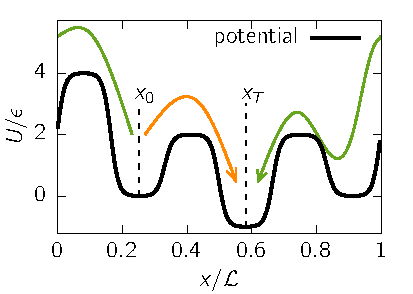
\includegraphics{../plots/Jaynes/potential_traj.pdf}
\caption[An example potential for a driven particle with periodic boundary conditions.]{An example potential, where the minima or chosen to be at position $s_{\textrm{min}}=\frac{3}{12}\,\mathcal{L}, \frac{7}{12}\,\mathcal{L}, \frac{11}{12}\,\mathcal{L}$ with potential minima  $U_{\textrm{min}}= 0\,\epsilon,-1\,\epsilon,0\,\epsilon$ respectively and maxima are at position $s_{\textrm{max}}=\frac{1}{12}\,\mathcal{L}, \frac{5}{12}\,\mathcal{L}, \frac{9}{12}\,\mathcal{L}$ with potential $U_{\textrm{max}}= 4\,\epsilon,2\,\epsilon,2\,\epsilon$ respectively. The green and orange arrow represent two different set of paths going from position $x_i$ to $x_j$. }
\label{fig:potential1D}
\end{figure}where $s_j$ shifts each summand of the potential to its chosen
position, $U_j$ denotes the potential of the $N$ local maxima or minima.
The potential has periodicity $p$ such that $U(x) = U(x+p)$
and $s_{N+1} = s_0 + p$. Parameter $k$ describes the smoothness of the
potential and is chosen as $k = -N \log \left( \frac{1}{0.999} -1
\right)$. $k$ should be chosen larger to minimise a force discontinuity at the periodic boundary. The potential becomes a set of Heaviside steps functions without discontinuity for $k \to \infty$. This potential allows us to construct a model with arbitrary barrier
heights, well depths, steepness of transition regions, and number and position
of wells and barriers. 
  
\subsubsection{Entropy Production}
\label{sec:Sprod}
We want to derive an expression for the local entropy productions $\Delta S_{ij}$ as introduced in \ref{sec:NESS}. The local entropy production of a single continuous trajectory $\mathbf{x}(t)$ is given by 
\begin{equation}
  \label{eq:deltaStraj}
  \Delta S [x (t)] = \int \dd {t} 
  \frac{ \mathbf{F} \cdot \mathbf{ \dot x}}{k_{\mathrm{B}}T},
\end{equation}
where  $\mathbf{ \dot x}$ is the velocity and $T$ is the temperature~\cite{seifert2005entropy}. Making use of numerically discretised trajectories from simulation, $\mathbf{x}(t) \approx \{\mathbf{x}_k\}$, $\Delta S$ is approximated between starting and target points $x_0$ and $x_T$, respectively,
\begin{equation}
 \Delta S[\{x_k \}]\approx \frac{1}{2T} \sum_d \sum_{t=1}^{t=T} \left ( x^{(d)}_t - x^{(d)}_{t-1} \right ) \left ( F^{(d)}({\mathbf{x}}_t) + F^{(d)}({\mathbf{x}}_{t-1}) \right ),
 \label{eq:SprodStr}
\end{equation}
where Stratonovich integration is used (see technical point~\ref{tec:Strat} ) and $d$ iterates over the dimensions.  

The solution above requires to integrate along trajectories and average over a trajectory ensemble. We approximate the  solution by ignoring the fluctuations, allowing us to apply Riemann integration. We make use of the analytic expression ${\mathbf{F}} = - \pdv{U({\mathbf ={x}})}{{\mathbf{x}}} + {\mathbf{f}}$ and find
\begin{equation}
\begin{aligned}
\Delta S [x (t)] &= \frac{1}{k_{\mathrm{B}}T} \int \dd {t} \sum_d \left ( \pdv{U}{x_d} \pdv{x_d}{t} + f_d \pdv{x_d}{t} \right )\\
 &= \frac{1}{k_{\mathrm{B}}T} \int \dd {t} \dv{U}{t} + \sum_d \left ( \int \dd {t} f_d \pdv{x_d}{t} \right )\\
 &=\frac{U(x_T) - U(x_0)  }{k_{\mathrm{B}}T} +  \sum_d \left ( \int \dd {t} f_d \pdv{x_d}{t} \right ) . 
\end{aligned}
\end{equation}
The non-conservative force $\mathbf{f}$ cannot be expressed by a potential and the integral depends on the path of $\mathbf{x}$. For the current 1D-case, two different sets of paths exist between $x_0$ and $x_T$ by using  the periodic boundaries as indicated in figure~\ref{fig:potential1D}. For equilibrium systems with $f=0$ both pathways have the same entropy production, otherwise there are two different solutions. By choosing the time-length of trajectories short, the longer path has negligible weight and we can assume a unique solution to the entropy production. The expression for the local entropy production becomes
\begin{equation}
  \Delta S(x_0,x_T) \approx \frac{ U(x_T) - U(x_0) + (x_T -x_0) f  }{ 
 k_{\mathrm{B}}T },
 \label{eq:Sprodth}
\end{equation}
only depending on start and endpoint of the trajectory. The solution of this equation differs from the solution of equation~$\ref{eq:SprodStr}$ by ignoring fluctuations and giving us an analytic estimate for the entropy production.  The path ensemble average of the entropy production is assumed to agree with the analytic solution as discussed in section~\ref{sec:Trajectory}. The approximated analytic solution is used throughout the thesis as it is much easier to solve. 



  
\section{Markov State Model}
\label{sec:MSM}
Markov State Modeling (MSM) aims to map the slow dynamics of a complex system to an underlying discrete Markovian process.
This involves several steps, including space discretisation, time discretisation and dimensional reduction \cite{bowman2013introduction}. The analysed models in this thesis are constructed such that space discretisation is performed manually.  All steps of the Markov State Model construction are presented on the minimal model introduced in the previous section~\ref{sec:1Dmodel}.

\subsection{Validate Markovian Process}
\label{sec:validate}
Markov processes were introduced in section~\ref{sec:MarkovProp}. An existing process is not bound to fulfill the Markov property so one has to check if it is met using the Chapman-Kolmogorov equation~\ref{eq:Chapman}. We focus on Markov state models of NESS, so the time-dependence on Markovian transition probabilities is dropped. A constant time-step length of each Markovian jump called \textit{lagtime} $\tau$ is assumed. The time-independent Chapman-Kolmogorov equation becomes
\begin{equation}
W(y_i | y_j , n \tau) = \int \diff y_1 \int \diff y_2 ... \int \diff y_{t}  W(y_1 | y_i , \tau) W(y_2 | y_1 , \tau) ...  W(y_j | y_{t} , \tau)
\end{equation}
for $t$ time steps and the transition probabilities depend on the lagtime. The state space of an MSM is discretised so we denote $W(y_i | y_j , \tau) = p_{ij}(\tau)$ as the jump probability from state $i$ to $j$ within time $\tau$. This quantity is estimated from simulation by choosing a lagtime $\tau$ and recording all jumps in a count matrix $c_{ij}(\tau)$. The transition matrix is estimated by
\begin{equation}
 p_{ij}(\tau) = \frac{c_{ij}(\tau)}{\sum_k c_{ik}}.
\end{equation}
In practice, it is cumbersome to check the Chapman-Kolmogorov equation for each element of the matrix $p_{ij}(\tau)$ so Prinz et al. \cite{prinz2011markov} suggested to expand the irreducible transition probability matrix $\hat p(\tau)$ in its eigenvalue decomposition
\begin{equation}
\hat p \boldsymbol{\Phi}_k = \lambda_k \boldsymbol{\Phi}_k .
\end{equation}
The time evolution of the probability distribution can then be described by 
\begin{equation}
 P(t) = \sum_k a_k \boldsymbol{\Phi}_k \exp \left ( -\ln (\lambda_k) t \right ),
 \label{eq:expansion}
\end{equation} 
where $a_k$ are constants that are determined by the initial state of the system. If the dynamics of the system fulfil detailed balance (i.e. the system is in equilibrium), the eigenvalues and eigenvectors are real and one can construct a hierarchy starting with the slowest process $\lambda_0 = 1 > \lambda_1 > ... > 0 $. Typically, the slow dynamical processes are of interested and the fast processes with small $\lambda$ are cut off from the expansion. The characteristic
timescales are identified from equation~\ref{eq:expansion} by $t_i = \frac{-\tau}{\ln \lambda_i}$ and are calculated for different lagtimes. Figure~\ref{fig:lagtime} shows an example of the slowest timescales for varying lagtimes for 60 microstates. The region where $t_i < \tau$ is forbidden because an observed timescale cannot be smaller than the minimal time-resolution of the Markov process.
The timescales reach a plateau for lagtime greater than $ 0.002\,\mathcal{T}$, indicating that the Chapman-Kolmogorov equation~\ref{eq:Chapman} is valid in this region: An MSM at a timescale $\tau_0$ is expected to describe the dynamics for $t > \tau_0$ , so it should agree with
an MSM parameterised at a lagtime $\tau_1 > \tau_0$ describing the same dynamics~\cite{swope2004describing}.  The timescale analysis is merely a tool to choose a lagtime for further analysis.
A test of consistency of the eigenvectors is needed for full conformation of Markovianity.
It is suggested to identify metastable states and compare detailed relaxation probabilities from the MSM to the error-analysed trajectory data. We start by defining the probability distribution of starting in a metastable state $A$ by
\begin{equation}
 \omega^A_i = 
   \begin{cases}
    \frac{\pi_i}{\sum_{j \in A} \pi_j} &\;\;\; i \in A\\
     0 &\;\;\; i \notin A .
   \end{cases}
\end{equation}
The probability of the measured trajectory data to remain in state $A$ after time $m\tau$ is then
\begin{equation}
 L_{\text{tr}}(A,m\tau) = \sum_{i \in A} \omega_i^A \frac{\sum_{j \in A} c_{ij} (m\tau)}{\sum_j c_{ij} (m\tau)},
\end{equation}
with the corresponding error 
\begin{equation}
 \varepsilon(A,m\tau) = \sqrt{m\frac{L_{\text{tr}}(A,m\tau) - \left( L_{\text{tr} }(A,m\tau) \right )^2 }{ \sum_{i \in A} \sum_j c_{ij} (m\tau)} } .
\end{equation}
If the MSM dynamics follows the Markovian relation
\begin{equation}
 \hat p (m \tau) \approx \left [ \hat p(\tau) \right ]^m,
\end{equation}
the result of iterating the MSM 
\begin{equation}
 L_{\text{MSM}}(A,\tau) = \sum_{i \in A} \left [ (\omega_i^A)^\top  [\hat p(\tau)]^m \right ]_i 
\end{equation}
should lie within the errorbars of the trajectory analysis by $L_{\text{tr}}(A,m\tau)$ with error $ \varepsilon(A,m\tau)$  . The method is shown on the 1D model in figure~\ref{fig:Cktest} for full conformation that the model defined by space discretisation and lagtime $\tau$ is Markovian for the slowest processes.
\begin{figure}
\centering
 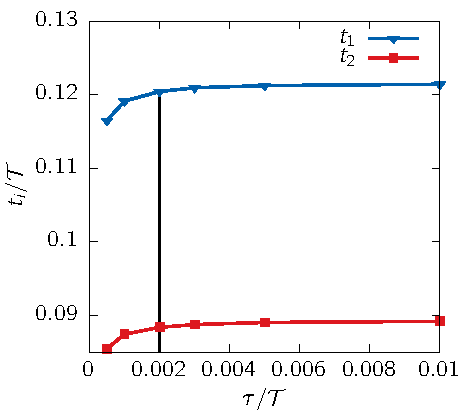
\includegraphics{../plots/MSM/lagtime_2010.pdf}
\caption[Two slowest timescales for the 1D driven system depending on lagtime.]{The slowest two timescales involved in the 1D system, depending on
the lagtime $\tau$ of the MSM. A lagtime of $0.002\,\mathcal{T}$ is chosen for the following analysis. }
\label{fig:lagtime}
\end{figure}

\begin{figure}
\centering
 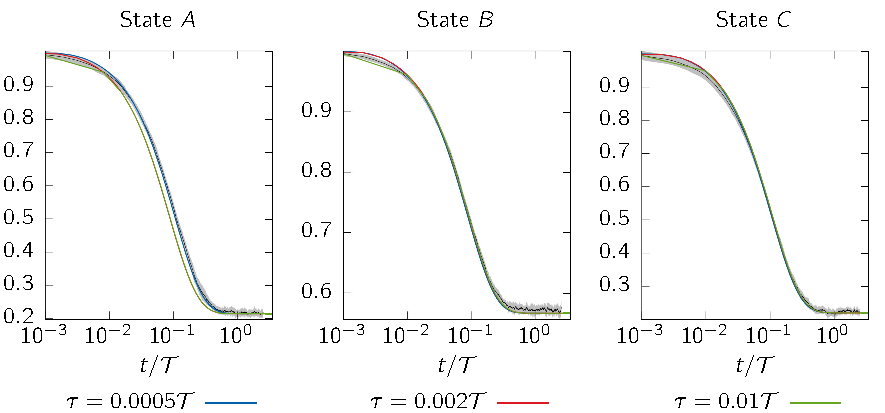
\includegraphics{../plots/MSM/cktest_2010.pdf}
\caption[Chapman-Kolmogorov test for the metastable states for the 1D driven system.]{Chapman-Kolmogorov test for the metastable states $A$,$B$,$C$ . The relaxation processes of the MSM at lagtime $\tau=0.0005\,\mathcal{T},0.002\,\mathcal{T},0.01\,\mathcal{T}$ agree well within the error of trajectory analysis shown by the grey shadow. }
\label{fig:Cktest}
\end{figure}


The eigenvalue decomposition allows detailed analysis of an MSM by isolating each process and showing detailed probability fluxes involved via the corresponding eigenvector.
The described methods rely on the transition probability matrix being reversible, where the eigenvalue decomposition is real-valued. In NESS this condition is not met and the eigenvalues may become
complex. A timescale separation with a hierarchy to delete fast processes with small real part of the eigenvalues is not possible~\cite{weber2017eigenvalues}. A similarly powerful tool
for analysis of NESS is not known yet, however the Schur-decomposition might be a good candidate for timescale separation~\cite{weber2015g}.
In this thesis, a reference equilibrium system is used to choose a lagtime for all driven systems using the same potential surface. First-passage-time-distributions (FPTD) (see section~\ref{sec:FPTD}) characterising the transition time distribution between two metastable states are used for analysis of the processes involved. 

\subsection{Identifying metastable states}
\label{sec:PCCA}
Depending on the number and definition of microstates physical interpretation of MSMs can become difficult. The resulting fine-grained transition matrix does hold all information, but we are only interested in the previously unknown long-term dynamics. The already coarse-grained dynamics can be further coarse-grained to its relevant states. The aim is to combine dynamically well-connected microstates to a macrostate while keeping the timescale of the transitions constant. An often applied method in the field of molecular simulation is the PCCA+~\cite{deuflhard2005robust}, an expansion to the earlier introduced PCCA~\cite{deuflhard1998identification}. We will shortly explain the workflow of PCCA and point out the addition made by PCCA+. 

\begin{figure}[t]
\centering
 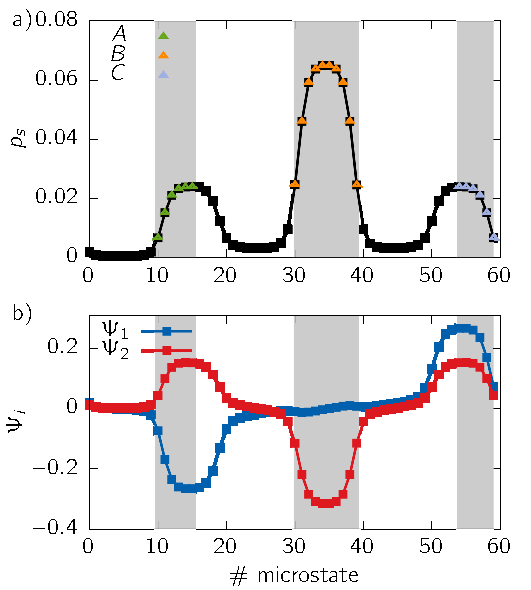
\includegraphics{../plots/MSM/Evec1.pdf}
 \caption{(a) Probability distribution for the equilibrium system with metastable states identified by PCCA+. (b) First and second eigenvector $\Psi_i$ representing the 
 probability flow during relaxation process. }
 \label{fig:Evec}
\end{figure}

By examination of the expansion of $P(t)$ in equation~\ref{eq:expansion}, one understands 
that the processes with $\lambda_i < 1$ vanish with time and only the stationary distribution $\Psi_0$ with $\lambda_0 = 1$ remains. The eigenvalue shows how fast the process annihilates in time, the corresponding eigenvector describes the corresponding probability flow. This is shown in figure~\ref{fig:Evec} for the 1D toymodel. The metastable states are already identified by $A$, $B$ and $C$. The probability flows from states where $\Psi_i$ is positive to the negative region or vice versa, depending on what is needed to reach the steady state. The first eigenvector exchanges probability between metastable state $A$ and $C$, the second between $B$ and $A$, $C$ equally, so the two flows 
cover all transition that one would intuitively expect from the system. 

PCCA makes use of the eigenvector by a hierarchical approach, starting with the eigenvector corresponding to the slowest process. The positive region of $\Psi_1$ is defined as one metastable state and the negative region as another. It continues using the second slowest eigenvector and applies it in the same manner to the metastable state, where it is most active. It proceeds in such a way that the number of metastable states is defined by the number eigenvectors taken into account. This approach is error prone due to large inactive regions where $\Psi_i \approx 0$, that are randomly assigned to one or another metastable state. PCCA+ corrects for this mistake by assuming all eigenvectors at the same time and assigning a membership probability $M$ for each microstate and each metastable state. A microstate between $A$ and $B$ would end up with membership of $M(A) \approx 50\,\%$, $M(B) \approx 50\,\%$ and $M(C) \approx 0\,\%$ due to its positioning as a transition state and should not belong to any metastable state. The states indicated in figure~\ref{fig:Evec}a each have membership $>95\%$ for a state. 

PCCA+ assigns metastable states that may not coincide with the maxima of a probability distribution as demonstrated for state $A$ and $C$. It is focused on making the metastable states dynamically connected, crisp and well separated while keeping the transition timescales between the metastable states constant. To apply the algorithm, the number of metastable states has to be chosen before running PCCA+. Another drawback is that it relies on the property that the 
eigenvalue expansion in equation~\ref{eq:expansion} is real, which only holds for equilibrium system. Similar to the Markovianity check, the metastable states are determined once for the equilibrium system and assumed to be valid for the driven system too. 

\subsection{First-Passage-Time Distribution}
\label{sec:FPTD}

%Include FPTD is more detailed than prinz CK test

First passage-times distributions (FPTD) are widely used to characterise processes in biology, chemistry and physics and are often associated with a free energy barrier a system has to overcome. The FPTD contains detailed transition information by collecting numerous realisations of a process. In experiment and simulation of rare events, the mean of the distribution is given due to limited observed process realisations~\cite{polizzi2016mean}.
Given an MSM with identified metastable states (see section~\ref{sec:PCCA}) the FPTD between all metastable states can be calculated. The collection of initial states is denoted by $I$, of final states by $F$.
For the purpose of calculating the FPTD~\cite{suarez2016estimating} from $I$ to $F$ the MSM is modified such that all final microstates $f \in F$ become a sink, i.e. all jumps out of the metastable state have probability 0 and staying in the state has probability 1
\begin{equation}
\begin{aligned}
\widetilde p_{fj} &= 0 \;\;\; &\forall j\neq f ,\;\;\; \forall f \in F& \\
\widetilde p_{ff} &= 1 \;\;\; &\forall f \in F&.
\end{aligned}
\end{equation}
An initial state is defined, where full probability is in one microstate $i \in I$ of the starting metastable state
\begin{equation}
\begin{aligned}
\rho_{i}^{(0)}  &= 1  \;\;\; & i \in I& \\
\rho_{j}^{(0)}  &= 0 \;\;\; &\forall j \neq i&.
\end{aligned}
\end{equation}
The probability distributions is iterated with the modified Markov model $\widetilde p$ until full probability is trapped in the sink. The superscript of $(t)$ denotes the number of iterations performed.
\begin{equation}
\rho^{(t+1)} = \widetilde p  \rho^{(t)} .
\end{equation}
The first-passage probability $p_{\;\text{FPT}}(t)$ at step $t$ is then the probability flow in the sink 
\begin{equation}
p_{\;\text{FPT}}(i \to F,t) = \sum_{l \in F} \rho^{(t)}_{l} - \rho^{(t-1)}_{l} .
\end{equation}
This calculation is repeated for all initial microstates $i \in I$. The full FPTD is then calculated by weighting each distribution with the weight $w_i$ of a trajectory starting in each initial microstate
\begin{equation}
w_i = \frac{ \sum_{k \notin I } \pi_k p_{ki} }{\sum_{i \in I} \left( \sum_{k \notin I } \pi_k p_{ki} \right ) } ,
\end{equation}
where $\boldsymbol{\pi}$ is the stationary probability distribution of a NESS. 
This expression adds up all probability flow to the initial state $I$ by 
$\sum_{k \notin I } \pi_k p_{ki}$ and normalises the probability of flowing 
into macrostate $I$. Note that this expression does not use the modified 
\begin{figure}[t]
\centering
 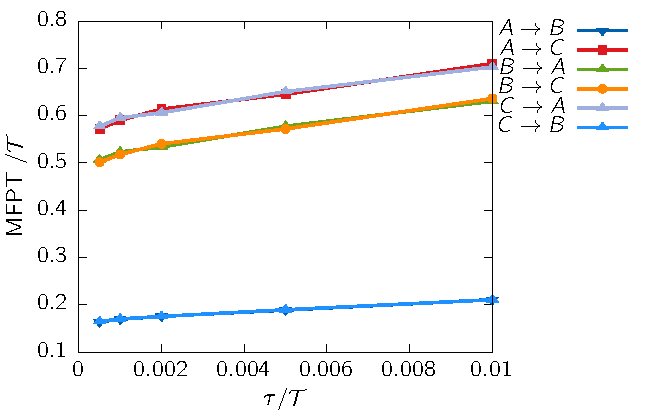
\includegraphics{../plots/MSM/tao_MFPT.pdf}
\caption[Mean first-passage time depending on the lagtime $\tau$ for all six observed processes for the 1D system.]{MFPT depending on the lagtime $\tau$ for all six observed processes. The model is designed such that groups of two processes overlap. The MFPT increases linearly with lagtime for all processes after a short period of faster growth.} 
\label{fig:tau_MFPT}
\end{figure} 
MSM. The full FPT can then be expressed by
\begin{equation}
p_{\;\text{FPT}}(I \to F,t)  = \sum_{i \in I} w_i p_{\;\text{FPT}}(i \to F,t)  .
\end{equation}
Knowing the FPTD, all moments of the distribution can be calculated by
\begin{equation}
M_{I \to F}^{(n)} = \sum_t p_{\text{FPT}} (I \to F,t) t^n.
\end{equation}
In particular we will make use of the quantities
\begin{equation}
 \begin{aligned}
  \mu_{I \to F} &= M_{I \to F}^{(1)} & \;\;\;\text{mean}& \\
  \sigma_{I \to F} &=  \sqrt{M_{I \to F}^{(2)} - \mu_{I \to F}^2 } & \;\;\;\text{standard deviation}& \\
  \kappa_{I \to F} &= \frac{ M_{I \to F}^{(3)} -3 \mu_{I \to F} \sigma_{I \to F}^2-\mu_{I \to F}^3 }{\sigma_{I \to F}^3}& \;\;\;\text{standardised skewness}& ,\\
 \end{aligned}
\end{equation}
where the standardised skewness is defined by the expectation value of $\left( \frac{t-\mu}{\sigma} \right )^3$.
The mean first-passage time (MFPT) was shown to be of special interested because it contains information about the transition rate between two states by the Hill relation~\cite{hill2005free}
\begin{equation}
 k_{I \to F} = \frac{1}{\mu_{I \to F}}.
\end{equation}
Similar to the timescale analysis and the Chapman-Kolmogorov test, the FPTD \begin{figure}[t]
\centering
 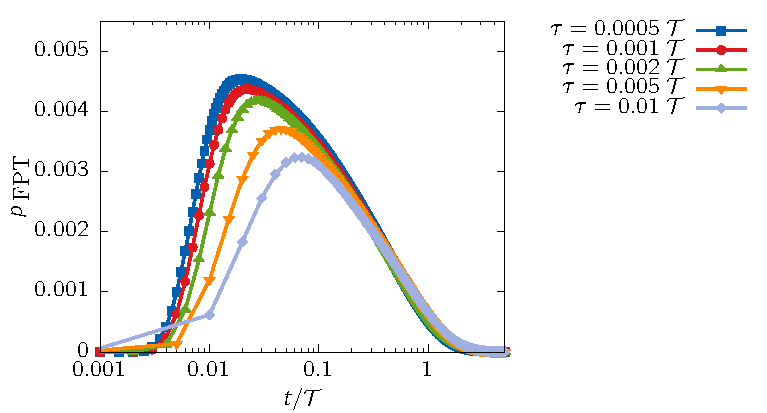
\includegraphics{../plots/MSM/tao_fpt.pdf}
\caption[First-passage time distribution of process from metastable state $B$ to $A$ at different lagtimes.]{FPTD of process from metastable state $B$ to $A$ at different lagtimes. The distributions are normalised such that they can be compared despite different resolution. The distributions do not cover each other, as one would expect from a perfectly Markovian process.}
\label{fig:tau_fpt}
\end{figure}
should not depend on the lagtime in the region of Markovianity. As shown in figure~\ref{fig:tau_MFPT}, this statement does not hold for the given system. The MFPT changes similar to the timescales in figure~\ref{fig:lagtime} up to a lagtime of $\approx 0.002\,\mathcal{T}$ but it continues to grow linearly after this point. The reason for this non-Markovian behaviour is shown in the detailed FPTD in figure~\ref{fig:tau_fpt}.
The increasing lagtime summarises processes that are shorter than $\tau$ but still contribute to the overall MFPT as a single jump and details on the process are lost. The distribution is distorted to slower processes and the MFPT grows. To avoid this problem, the lagtimes should be chosen according to the criterions on Markovianity but as short as possible to keep details on the dynamics. The observed non-Markovianity is detected because the first-passage time is an even stronger test of Markovianity than the test performed in section~\ref{sec:validate}. It analyses transitions between two metastable states and not just the exit from one. The presented exit test is used because it benefits from small error by making use of larger sample sizes. Many trajectories remain in the metastable state for a while. The error increases with time when the amount of trajectories remaining in the basin is small. The error for the FPTD is always large because it requires many incidents of the same transition time and a statistical analysis becomes cumbersome. Irrespective of the discussion of statistical applicability, the non-Markovianity of MFPT raises the question if it is a good quantity for comparison of simulation, MSM and experiment 


 


% 
% 
% 
% % 
% \bibliography{/home/marius/PhD/Thesis/references.bib}
% \bibliographystyle{plain}
% \end{document}
 
% 
% %\documentclass[paper=a4,fontsize=12pt,open=right,noabbrev]{report}
% \documentclass[12pt]{report}
% \usepackage[utf8]{inputenc}
% \usepackage{amsmath}
% \usepackage{amssymb}
% \usepackage{graphicx}
% \usepackage{cite}
% \usepackage{physics} 
% \usepackage{mathrsfs}
% \newcommand*\diff{\mathop{}\!\mathrm{d}}
% \usepackage{geometry}
% \usepackage{layouts}
% \usepackage{newfloat}
% \usepackage{float}
% \usepackage{listings}
% \usepackage{bm}
% \usepackage{csquotes}
% 
% \setlength{\parindent}{0em}
% \setlength{\parskip}{1em}
% 
% \lstset{language=Python,basicstyle={\ttfamily }}
% 
% %% Technical point floatstyle
% \floatstyle{ruled}
% \newfloat{Technical Point}{htbp}{lop}[chapter]
% 
% 
%  

%\begin{document}

\chapter{Jaynes Maximum Caliber}
\label{ch:Jaynes}
Edwin Thompson Jaynes discussed the question of the possibility of macroscopic 
prediction from microscopic information of a system~\cite{jaynes1985macroscopic}. He based 
his work on the earlier theory of  Boltzmann's statistical 
mechanics~\cite{boltzmann1896vorlesungen}. Boltzmann stated that the entropy 
is the crucial key to connect microscopic and macroscopic phenomena --- and that the 
lack of understanding a macroscopic phenomena might be caused 
by ignoring the effect of the entropy. Boltzmann connected the two worlds by 
the simple identity $S = k_{\textrm{B}} \ln{W}$, where the 
left-hand side  is the macroscopic property entropy, known from equilibrium thermodynamics, and the right-hand side counts the number of microscopic 
configurations. The argumentation transformed time-dependent trajectories to a 
collection of microstates and thus ergodicity was demanded. 

Gibbs introduced the idea of probabilities of a microstate 
$i$ in an entropic 
system in the form of $S = -k_{\mathrm{B}} \sum_i p_i \ln p_i$. He changed the point of view by the introduction of ensembles with certain thermodynamic characteristics, like constant temperature or pressure. 
The ensembles allow us to observe a number of identical non-interacting systems with the same macroscopic parameters instead the time-evolution of a single system. The axiom of \textit{equal a priori probabilities} becomes necessary. It states that all known states have the same probability without further knowledge of the system to connect the independent system, i.e. $p_i = \frac{1}{W}$. The Gibbs formulation of the entropy reduces to Boltzmann's formula 
\begin{equation}
\begin{aligned}
 S &= -k_{\mathrm{B}} \sum^W_i p_i \ln p_i \\
 & = -k_{\mathrm{B}} \sum^W_i \frac{1}{W} \ln \frac{1}{W} \\
 & =k_{\mathrm{B}} \ln W,
\end{aligned} 
\end{equation}
meaning that Boltzmann's equation holds for no additional thermodynamic information. In the Gibbs formulation, the entropy decreases if information are given,   resulting in probabilities of microstates that differ from one another. He shows how to introduce statistical ensembles (see section~\ref{sec:EnsembleAv}) in equilibrium by maximising the entropy with respect to certain constraints~\cite{gibbs1902elementary}. He claims that a statistical system is observed in a state where it has the most microscopic realisations available while satisfying macroscopic constraints. Other states may agree with these constraints but are entropically suppressed and are thus negligible. 
 
\begin{Technical Point}[t] 
\begin{minipage}{0.03\textwidth}
\hfill\vspace{0.1cm}
\end{minipage}%
\begin{minipage}{0.4\textwidth}
 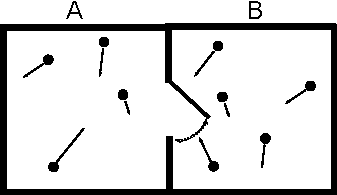
\includegraphics{../images/maxwell.pdf}
\end{minipage}
\hfill
\begin{minipage}{0.55\textwidth}
  Maxwell proposed a gedankenexperiment that seemingly opposes the second law of thermodynamics. He assumed two boxes A and B that are filled with particles and only connected by a door that can be opened and closed.  Assuming the existence of a all-knowing conscious --- the demon --- it could open the door whenever a fast particle passes from  box A to B and close
  it otherwise. In the other direction,  it could \vspace*{0.055cm} \end{minipage}  open the door whenever a slow particle wants to pass from box B to A and close it otherwise.
  The door operates frictionless. The box A would cool down and B would heat up --- opposing the second law of thermodynamics which demands that two objects in contact evolve to an equilibrium with both objects at the same temperature~\cite{leff2014maxwell}. \\
  
  It is believed that the laws of thermodynamics are not violated, but it follows that a source of the missing entropy production, to fulfil $\delta S \ge 0$, is missing. The source is found in the demon itself, which interacts with the system by measurement and by storing data. The measurement can be ruled out because it was shown to be possible by a reversible process~\cite{landauer1961irreversibility}. A solution identified by Bennett states that the demon eventually runs out of data storage and has to delete gathered information~\cite{bennett1987demons}. Laundauer showed that deleting one bit increases the entropy by $S_{\text{bit}} = k_{\mathrm{B}}\ln 2$~\cite{bennett2003notes}. The gedankenexperiment of Maxwell's Demon provides us with a way to think of the connection of information and physical entropy.  
  \caption{Maxwell's Demon}\label{tec:Maxwell}
\end{Technical Point}
 
Shannon introduced the information-theoretic entropy for a probability distribution given by $S = \sum_i p_i \log_2 p_i$, only differing from the Gibbs entropy by the factor of $k_B \ln 2$~\cite{shannon1948mathematical}. 
The Gibbs entropy can be seen as the amount of Shannon entropy required to define the microscopic state of a system. The reverse consequence --- that the possession of microscopic information must have thermodynamic consequences --- was formulated in the form of the famous Maxwell Demon~\cite{bennett1982thermodynamics} (see technical point~\ref{tec:Maxwell} ). Jaynes accepted the similarity of information and thermodynamic entropy without proof and proposed to generalise the Gibbs algorithm from thermodynamic systems to all probabilistic systems. In a first step, he formulated this idea for equilibrium systems \cite{jaynes1957information}, later he extended it to time-depending off-equilibrium  systems~\cite{jaynes1985macroscopic}. His idea is to move from a physical deductive theory for thermodynamics to an inferent theory: A deductive theory predicts what will happen, whereas the inference theory proposes the most likely probability distribution based on given data and information. 
He also argues from a practical way that most real systems are 
too complex for a deductive proof with definite predictions. Most important 
is the correct identification of macroscopic parameters that reduce the information entropy to a significant distribution of microstates. From the remaining probability distributions that fulfill the constraints, the one with the highest entropy (or least information) is chosen to be as non-committal as possible with regard to unknown information. Insignificant information 
on the other hand will barely change the outcome compared to the prior information.
This information-theoretic argumentation allows to drop the assumption of equal a priori probabilities and ergodicity. The first assumption is now a product of the theory in case when no information are available: The entropy function $-k_{\mathrm{B}} \sum^W_i p_i \ln p_i$ has a global maximum for equal probabilities $p_1 = p_2 =\dots=p_W$.  The second assumption of ergodicity was initially introduced to describe equilibrium systems by their microstates instead of time-dependent trajectories.  The shift from a physical theory to an information theory makes this assumption obsolete. We may apply the theory to any kind of probabilistic systems including fields in physics, biology, economics and more. 

Later, Shore and Johnson changed the point of view on the maximum entropy assumption once more: They showed that the entropy function by Shannon is the only function that fulfils logical requirements of inference, 
as it will be shown in the following section~\ref{sec:inference}. It proves that the argument of maximising the uncertainty of Jaynes is not needed anymore. The maximum uncertainty is a necessary criterion for a consistent inference method. 

Depending on the situation of the inference task, one might 
use any of the given interpretation by Gibbs, Jaynes or by Shore and Johnson. 
The Gibbsian point of view is motivated by physics and provides a good 
basis for the interpretation of equilibrium statistical physics. Jayne's method 
allows an interpretation of all fields beyond equilibrium physics, whereas Shore's and Johnson's addition to the theory base it on a solid logical ground but is less applicable for a physical interpretation. This thesis uses the name \textit{Maximum Caliber} for historical reasons, although other mathematicians and physicists than Jaynes contributed to understanding the method.  



\section{Requirement for uncertainty measures and inference methods}
\label{sec:inference}
% uncertainty measure - NOT fulfiled by Bayes? % shift to KL-diveregence
% SJ : properties of inference method - Is this fulfilled by Bayes?
There are numerous functions that may be considered as a measure for uncertainty.
This thesis focuses on the relative entropy as defined by Kullback and Leibler 
$ \int_X \dd{X} P(X) \ln \frac{P(X)}{Q(X)}$, where $Q(X)$ represents the assumed distribution called \textit{prior} in Bayesian statistics. $P(X)$ is the probability distribution assigned based on the data and constraints, called \textit{posterior}~\cite{jaynes2003probability}. It fulfils the axioms an uncertainty measure should meet as formulated by Hobson~\cite{hobson1973comparison} as an extension to Shannon's axioms~\cite{shannon1948mathematical}. 
The extension was necessary to include known data that 
was not considered by the entropy definition of Jaynes. 
The uncertainty measure is denoted by $S(P(X)|Q(X))$, where
the probability of outcome $X= (x_1, x_2,...,x_N)$ is $P(X)$, assuming prior $Q(X)$. An uncertainty measure should fulfil the following axioms:
\begin{itemize}
 \item 1. $S(P(X)|Q(X))$ is continuous in $P(X)$ and $Q(X)$.
 \item 2. $S(P(X)|Q(X))$ does not depend on how the outcome $x_1,x_2, ... , x_N$ 
 are labeled.
 \item 3. $S(P(X)|Q(X)) = 0$ if $P(X) = Q(X)$ 
 \item 4. When $Q(X) = (n_0^{-1}, n_0^{-1} , ... , n_0^{-1})$ and 
 $P(X) = (n^{-1}, n^{-1} , ... , n^{-1},0,...,0)$ $(n \leq n_0)$ then 
 $S(P(X)|Q(X))$ is an increasing function of integer $n_0$ and decreasing function of $n$.  
\item 5. If $Y$ denotes additional states and $P(X,Y)$ and $Q(X,Y)$ denote the 
joint probabilities, then the uncertainty of the composite system should be expressed as
\begin{equation}
   S(P(X,Y)|Q(X,Y)) = S(P(X)|Q(X)) + \sum_i P(x_i) S(P(Y | x_i) | Q(Y | x_i)) % is this correct..? 
\end{equation}
\end{itemize}
The first three axioms are reasonable, only defining a continuous function with a minimum whenever $P(X)$ equals $Q(X)$, meaning no new information are given  
and the ordering of learning new variables does not matter.
The forth axiom states that uncertainty decreases if states can be deleted and increases if states 
are introduced. 
% think about the last axiom
The last axiom defines the extension of correlated systems, where 
the uncertainty should grow with additional states $y_i$ consistent with the conditional probability $p(y_1,..., y_M | x_i)$.
The Kullback-Leibler entropy in the form of
\begin{equation}
 S(P(X)|Q(X)) = \int \dd{X}  P(X) \ln \frac{P(X)}{Q(X)} 
\end{equation}
is the unique functional form for an uncertainty measure fulfilling above axioms. The negative Kullback-Leibler divergence (or relative entropy) reduces to the Shannon entropy 
if the prior is equi-distributed~\cite{shannon1948mathematical}.
Hobson shows that the Kullback-Leibler divergence has a unique minimum for $Q(X) = P(X)$ and it is convex in the sense of probability mass functions. 
To apply Jaynes theory, we will use a prior to include data on the system and constraints in the form of Lagrangian multipliers to infer physical information. The result of this inferring process should follow some axioms too, as formulated and proven for the Kullback-Leibler divergence by Shore and Johnson~\cite{shore1980axiomatic}:
\begin{itemize}
 \item Uniqueness: The result should be unique.
 \item Invariance: The result is independent of the choice of the coordinate system.
 \item System Independence: Independent information about independent systems can be inferred separately in terms of different densities or together in terms of joint densities.
 \item Subset Independence: Independent subsets of system states can be treated in terms of a separate conditional density or in terms of the full density. 
\end{itemize}
All axioms together lead to the Kullback-Leibler divergence as the unique consistent candidate for inferring information on a set of data. We showed before that it is also a function for uncertainty measurement, supporting Jaynes intuitive interpretation of choosing the system of highest uncertainty under defined constraints.
 
The assumptions made above do not require equilibrium of any kind. We will continue 
to show how the Maximum Caliber with an equilibrium assumption is used to derive ensembles in statistical mechanics and continue by generalizing to off-equilibrium steady states. 

\section{Reweighting in Equilibrium}
 \label{sec:rewEqu}

The following derivation shows how Jaynes principle is used to recover data reweighting (see section~\ref{sec:EnsembleAv}), a method that was first described by Swendsen and Ferrenberg and is frequently used for simulation~\cite{ferrenberg1988new}. 
According to Gibbs statistical ensembles, a canonical ensemble (or $NVT$ ensemble) is defined by a closed system of constant volume, that does not allow particle exchange with its surrounding and is connected to an infinitely large reservoir with constant temperature and can exchange energy with it. Applying Jaynes theory, we infer the macroscopic average energy of the system. 
It is assumed that microscopic data is available from previous measurements in form of $q(x)$, where $x$ is a microstate with Energy $E(x)$. Considering the information, the Caliber is denoted by
\begin{equation}
\begin{aligned}
\mathcal{C_{\text{equ}}} = -\int \diff x \; p(x) \ln \left ( \frac{p(x)}{q(x)} \right )  - \zeta \left ( \int \diff x \; p(x) - 1 \right ) \\
- \beta \left( \int \diff x \; p(x) E(x) - \langle E \rangle \right),
\end{aligned}
\label{eq:Caliber1}
\end{equation}
where $\zeta$ and $\beta$ denote Lagrangian multipliers and the probability distribution $p(x)$ is normalised to $1$.  Functional maximisation $\fdv{\mathcal{C_{\text{equ}}} }{p(x)} = 0$ yields 
\begin{equation}
 p(x) = q(x) \exp \left ( -1 - \zeta -\beta E(x) \right ).
\end{equation}
Enforcing normalisation to $1$ gives an expression for the corresponding Lagrangian multiplier $\zeta$. One finds an expression for the new probability distribution that depends on $\beta$
\begin{equation}
    p(x) =  \frac{q(x) \exp \left ( -\beta E(x) \right )}
    {\int \diff x q(x) \exp \left( -\beta E(x) \right ) }. 
\label{eq:RewEqu}
\end{equation}
This is the reweighting formula for reference data $q(x)$ to $p(x)$ based on a change in the average energy. From equilibrium statistical mechanics (see section~\ref{sec:EnsembleAv}) we know that the Lagrangian multiplier $\beta$ can be identified with the inverse temperature  $ \frac{1}{k_{\textrm{B}}T}$ that controls the average energy in a canonical ensemble. The reweighting procedure connects the probability distributions at different temperatures. 
\begin{Technical Point}[t]
\begin{minipage}{0.03\textwidth}
\hfill\vspace{0.1cm}
\end{minipage}%
\begin{minipage}{0.3\textwidth}
    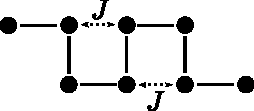
\includegraphics{../images/ISAW.pdf}
\end{minipage}
\hfill
\begin{minipage}{0.65\textwidth}
The self-avoiding walk (SAW) was introduced by Paul Flory to model chain-like polymers~\cite{flory1953principles}. The polymer is mapped on a grid where each site represents one monomer. An already occupied site cannot be \vspace*{0.055cm} \end{minipage} occupied  by another monomer to model the self-excluding interaction. An interaction between close-by monomers is introduced by an attractive potential between monomers on neighbouring sites. For $n_b$ bonds of strength $J$ one finds the energy


\begin{equation}
 E = -J n_b .
\end{equation}
The model can be constructed on different grids, however their effects on the system vanish in the thermodynamic limit~\cite{de1979scaling}. The SAW was studied in various dimension,  with different interaction range or close to surfaces and has become one of the most-studied models in polymer physics~\cite{vanderzande1998lattice}. 
  \caption{Interacting Self-Avoiding Walk}\label{tec:ISAW}
\end{Technical Point}
It can be understood by assuming that the reference data was sampled from a canonical ensemble at temperature $T'$, i.e. $q(x) = \exp \left ( \frac{-E(x)}{k_{\mathrm{B}} T'} \right )$. Plugging this into equation~\ref{eq:RewEqu}  shows that 
\begin{equation}
     p(x) =  \frac{ \exp \left [ \left ( -\frac{1}{k_{\mathrm{B}} T} - \frac{1}{k_{\mathrm{B}} T'} \right )E(x) \right ]}
    {\int \dd{x} \exp \left [ \left ( -\frac{1}{k_{\mathrm{B}} T} - \frac{1}{k_{\mathrm{B}} T'} \right )E(x) \right ] }
\end{equation}
is the probability distribution at a a new temperature $T'' = \frac{1}{\frac{1}{T'}+\frac{1}{T}}$. We conclude that the chosen temperature $T$, or the Lagrangian multiplier $\beta$, in the reweighting procedure is the change in temperature from the reference data. Making use of the density of states $\Omega(E)$ the reweighting equation~\ref{eq:RewEqu} recovers the known relation 
\begin{equation}
     p(E) =  \frac{ \Omega(E) \exp \left [ \left ( -\frac{1}{k_{\mathrm{B}} T''} \right )E \right ]}
    {\int \dd{E} \Omega(E) \exp \left [ \left ( - \frac{1}{k_{\mathrm{B}} T''} \right )E \right ] }.
\end{equation}
Here we assume that the density of states is fully known. However, since we only have access to the reference data $q(x)$ the density of states is only estimated over a sampled region by
\begin{equation}
 \Omega(E) \approx \int \dd{x} \delta(E(x) - E) \exp \left ( \frac{E(x)}{k_{\mathrm{B}} T} \right ).
\end{equation}
This sampling issue is illustrated in figure~\ref{fig:ISAW} on simulation data of 3 different temperatures of the interacting self-avoiding walk (see technical point~\ref{tec:ISAW}). The reference energy histogram $q(E)$ sampled at $8 \frac{J}{k_{\mathrm{B}}}$ is reweighted to the histograms $p(E)$ at the temperatures  $4 \frac{J}{k_{\mathrm{B}}}$ and $5 \frac{J}{k_{\mathrm{B}}}$. The result is compared to simulation data at the target temperature. The reweighting to $5 \frac{J}{k_{\mathrm{B}}}$ shows good results. The deviations are due to statistical noise of the simulation data. Reweighting to temperature $4 \frac{J}{k_{\mathrm{B}}}$, on the other hand, shows a large deviation compared to the target histogram. The issue is that states below $-80 J$ are not sampled by the reference simulation and the estimation of the density of states is flawed in this region. The reweighting procedure relies on data and produces wrong results if these are unavailable. Furthermore, one does not know initially what states have to be sampled to reweight to a certain temperature.  A careless use of the method can result in large errors in the analysis.


\begin{figure}

 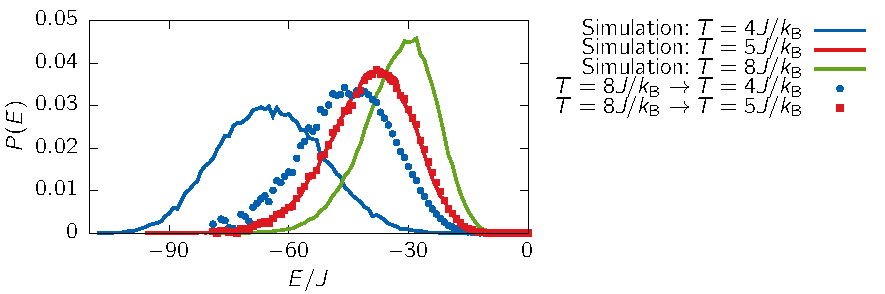
\includegraphics{../plots/Jaynes/ISAW.pdf}
 \caption[Equilibrium-reweighted energy distribution of the interacting self-avoiding walk.]{The energy distribution of the interacting self-avoiding walk of length 100 on 3-dimensional cubic lattice at three temperatures. Temperature reweighting is applied to the data from a simulation at $T = 8 \frac{J}{k_{\textrm{B}}}  $ to recover the other two distributions. 
 } \label{fig:ISAW}
\end{figure}

The reweighting example discussed above is applied with respect to energy in a canonical ensemble. However, the theory allows to define and reweight within any kind of ensemble. In this sense, one might constrain the number of particle $N$ in a system and extend the reweighting to grandcanonical ensembles using Jaynes Maximum Caliber. One might as well think of defining a new ensemble by radius of gyration $R_g$, which is used as an order parameter for the collapse transition of this model. The reweighting procedure works if the experiment or simulation producing reference data is set up such that the correct ensemble is sampled. In particular one would have to introduce a new thermostat, imitating these fluctuations on $R_g$. Such an ensemble is model-dependent and thus not used commonly. On the other hand it illustrates the number of options one has to define ensembles beyond the commonly used ones. This freedom in choosing controlling parameters will be handy when entering ensembles of NESS. 



\section{Reweighting in Off-Equilibrium}
\label{sec:RewOffEqu}
The Maximum Caliber Principle of Jaynes is shown to be a powerful tool --- both for the definition of known and unknown statistical ensembles and for the reweighting of existing data to fit new constraints. The previous section focused on the case that the system is in equilibrium. In the sense of the thermodynamic laws, it means that the change of entropy on average is zero. The entropy of the system, defined in equilibrium statistical mechanics, is a state function $S_{\text{sys}}$, determined by the density of states. Considering internal dynamics, the system might increase its entropy $\dd{S_{\text{sys}}}$ by a bit by borrowing heat from a thermal bath.  This is the \textit{system} entropy production on the state function $S_{\text{sys}}$. If the system returns to its initial state, it releases the same amount of entropy to the heat bath. The system is considered in equilibrium with its heat bath, if the \textit{medium} entropy production $\dd{S_{\text{med}}}$ along this process in the heat bath is zero too. In this case, the \textit{total} entropy production $\oint \dd{S_{\text{tot}}}$ along any circular trajectory is $\oint \dd{S_{\text{med}}}+ \oint\dd{S_{\text{sys}}} =0$. It implies that the change of entropy in the system $\int \dd{S_{\text{sys}}}$ along any trajectory only depends on the starting and endpoint, so that the process is path-independent. 

Equilibrium is a strict condition on the full system and is not always fulfilled. For instance, an outside observer may accelerate particles in one direction and thus performing work on the system. The additional 
energy may remain in the system or dissipate via a reservoir. In any case, there will be an increase of entropy in the bath or the system and presumably a reduction of the observer's entropy. In a similar picture, the system might be connected to two reservoirs of different temperature accelerating and slowing down the dynamics of the system, respectively. For instance, when entropy is increased by transferring heat from the hot reservoir to the system in kinetic energy of particles, the heat is unlikely to be transferred back. There is a possibility of back transferring for trajectories with much lower probabilities than the forward process (see in section~\ref{sec:StochTherm}).  These systems are examples of off-equilibrium where $\oint \dd{S} > 0$, on average.  The amount of entropy produced is path-dependent, i.e., it depends on the internal dynamics of the system. This system cannot be defined by the entropy because it is a function on the current state of the system alone. Entropy productions are defined including the interaction with the reservoir and describe the change of the system along a single trajectory. 

The Caliber for equilibrium systems in the previous section was defined for microstates because path-dependencies can be dropped for the description of the thermodynamic state. Trying to define the Caliber for off-equilibrium processes, we have to use \textit{microtrajectories} $\Gamma$ because these define the thermodynamic state now, as discussed above. A microtrajectory consists of a time series of microstates of the system.  In accordance with Jaynes generalised view on entropy maximisation to all existing statistical systems, we may sum over all microtrajectories in the system for a relative path entropy:
\begin{equation}
    \mathcal{C_{\text{tra}}} = \sum_\Gamma^{\text{trajectories}} p_\Gamma \ln \frac{p_\Gamma}{q_\Gamma} .
    \label{eq:traC}
\end{equation}
The task of the maximum Caliber is now to find the best possible distribution of microtrajectories in accordance to the yet to be defined constraints. Some questions are raised:
\begin{itemize}
    \item The phase space is defined over all possible trajectories. How can one assign a probability to each microtrajectory? 
    \item Microtrajectories are time-consuming to sample. Increasing the trajectories' length generates a unreasonably large number of trajectories to consider. 
    Can one limit the number of trajectories to a computational accessible level? 
    \item Off-equilibrium systems are physically different to equilibrium systems and need 
    new constraints. The canonical ensemble constraint cannot be used anymore because energy is a state function and cannot be uniquely defined for trajectories. What constraints apply for off-equilibrium? 
    \item The density of states is a fundamental invariant measure for equilibrium statistical mechanics. Is there a similar quantity for trajectories?
\end{itemize}
All these questions will be discussed in the following for the case of a non-equilibrium steady state (see section \ref{sec:NESS}). These are a special case of off-equilibrium  because heat is supplied to the system from an unlimited reservoir and withdrawn at the same rate. The system will eventually settle in a state with a constant total entropy production  $\dd{S_{\text{tot}}}>0$ but the system does not undergo changes; it is in a steady state with $\dd{S_{\text{sys}}} =0$. The entropy is produced purely by the reservoir driving the system and the reservoir withdrawing heat from the system. This results in system trajectories weights that are time-independent, as the system itself does not undergo changes. At the same time, the total system produces entropy, keeping the phenomena of non-equilibrium. 

The question of assigning probabilities to a diverging number of trajectories is addressed via Markov state modeling as discussed in section~\ref{sec:MSM}. The probability of observing a trajectory $\Gamma$ is replaced by a Markovian discretised trajectory of the form 
 $p_\Gamma \approx \sum_{\{i_{0}, i_{1}, \cdots , i_{T} \}} \pi_{i_0} p_{i_0 i_1} \cdots p_{i_{T-1} i_{T}} $,
where $\pi_{i_t}$ is the probability to be in state $i_t$ at time point $t$ and 
$p_{i_{t} i_{t+1}}$ is the conditional probability to jump from state $i_{t}$ to $i_{t+1}$ from time-point $t$ to $t+1$. The prior $q_\Gamma$ is similarly approximated with initial distribution $\rho_{i_t}$ and transition probability $q_{i_{t} i_{t+1}}$. We find the Markovian form of equation~\ref{eq:traC}:
\begin{equation}
    \begin{aligned}
    \mathcal{C_{\text{Markov}}} & = \sum_{\{ i_0, i_1 , \cdots , i_T \}} \pi_{i_0} 
     \left ( \prod^{T-1}_{k}  p_{i_k i_{k+1}} \right) \left ( \ln \frac{\pi_{i_0}}{\rho_{i_0}} 
    + \sum^{T-1}_{l} \ln \frac{p_{i_l i_{l+1}}}{q_{i_1 i_{l+1}}}  \right ) \\
    & = \sum_{\{ i_0, i_1 , \cdots , i_T \}} \pi_{i_0} 
    \left ( \prod^{T-1}_{k}  p_{i_k i_{k+1}} \right)  \ln \frac{\pi_{i_0}}{\rho_{i_0}} \\
    &\;\;\;\;+ \sum^{T-1}_{l} \sum_{\{ i_0, i_1 , \cdots , i_T \}} \pi_{i_0} 
    \left ( \prod^{T-1}_{k}  p_{i_k i_{k+1}} \right) \ln \frac{p_{i_l i_{l+1}}}{q_{i_1 i_{l+1}}}\\ 
    & = \sum_{i_0} \pi_{i_0} \ln \frac{\pi_{i_0}}{\rho_{i_0}} + \sum^{T-1}_{l} \sum_{\{ i_0, i_1 , \cdots , i_T \}} \pi_{i_0} 
    \left ( \prod^{T-1}_{k}  p_{i_k i_{k+1}} \right) \ln \frac{p_{i_l i_{l+1}}}{q_{i_1 i_{l+1}}}\\ 
    & = \sum_{i_0} \pi_{i_0} \ln \frac{\pi_{i_0}}{\rho_{i_0}} + 
    \sum^{T-1}_{l} \sum_{\{ i_l, i_{l+1} \}} \pi_{i_l} p_{i_l i_{l+1}} 
    \ln \frac{p_{i_l i_{l+1}}}{q_{i_l i_{l+1}}}\\
    & = \sum_i \pi_{i} \ln \frac{\pi_{i}}{\rho_{i}} + T \sum_{i,j} \pi_i p_{ij} 
        \ln \frac{p_{ij}}{q_{ij}}\\
    & \approx T \sum_{i,j} \pi_i p_{ij} \ln \frac{p_{ij}}{q_{ij}} .
\end{aligned}
\end{equation}
The first line represents the Caliber when the Markovian description is plugged in and trajectories are assumed to be time dependent. The brackets are multiplied and the order of the sums of the second term is interchanged. The third line uses the probability conservation $\sum_{i_{k}} p_{i_{k-1} i_{k}} =1$ starting with the last sum over $i_T$ until only the sum over $i_0$ remains. A similar trick is applied in the next step on the second term, only now the first sum is solved over $i_0$ and global balance $\sum_{i_{k}} \pi_{i_k} p_{i_{k} i_{k+1}} = \pi_{i_{k+1}}$ is used iteratively. The assumption of global balance is that the system's probability distribution does not change in time and is in a NESS. The fifth line relabels the indices because the explicit time-dependence is not needed for NESS. The approximation assumes $T$ being large, meaning that the input trajectory should be long in order to forget the initial state. The remaining $T$ is just an arbitrarily large factor and is ignored for the maximisation process. The trajectories consist of contribution from the stationary distribution $\bm{\pi}$ and the transition probabilities $p_{ij}$ so the maximisation has to be performed over both quantities.  


\subsection{Theory of Constraints}
Having convinced ourselves that the Maximum Caliber is indeed a general tool for data inference, we advance to the question of how to constrain the Caliber for off-equilibrium processes. Unfortunately it is not yet known what quantities control the outcome of a non-equilibrium experiment and thus a general theory has not been found yet~\cite{maes2018non}. However, the Maximum Caliber provides a perfect testing ground to investigate certain assumptions and control their outcome by simulation or experiment. The constraints can be distinguished in groups with certain properties:
\begin{itemize}
 \item intensive / extensive constraints
 \item symmetric / asymmetric constraints with respect to heat exchange with the reservoir under time reversal and space inversion
 \item local / global constraints 
\end{itemize}
We start by discussing extensive quantities, growing proportional to the system size. It was shown that extensive quantities are sufficiently constrained by their first order~\cite{dixit2018perspective}: An extensive quantity in systems $A$ and $B$ adds up when bringing both systems together, e.g. the Energy
$\langle E \rangle_{\text{tot}} = \langle E \rangle_{A} + \langle E \rangle_{B}$. 
This means that fluctuations are allowed but are subdominant and higher orders 
are negligible. Constraining these quantities in higher order is not necessary. Intensive quantities on the other hand can be constrained on higher orders to improve the result of inference. We wish to avoid higher order constraints because they suffer from larger statistical error. 

\begin{figure}
 \centering

 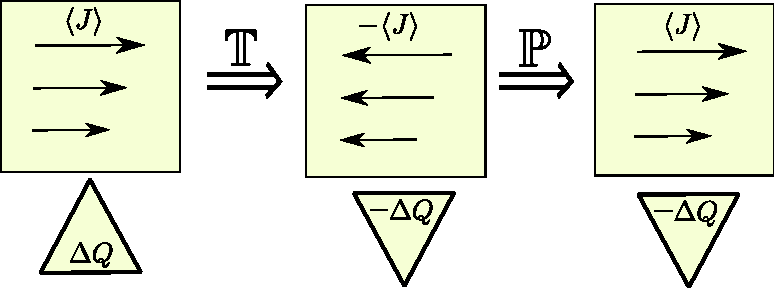
\includegraphics{../images/PT-Transform.pdf}
 % PT-Transform.pdf: 372x138 px, 72dpi, 13.12x4.87 cm, bb=0 0 372 138
 \caption[Illustration of symmetric and asymmetric observables under time reversal and space inversion. ]{Illustration of observable mechanical flux in the system $\langle J \rangle$ and heat exchange with a reservoir $\Delta Q$ under 
     time reversal $(\mathbb{T})$ and space inversion $(\mathbb{P})$. The mechanical flux 
     is symmetric under $\mathbb{P}\mathbb{T}$-transformation, the heat exchange is anti-symmetric. }
 \label{fig:PTtransform}
\end{figure}

Jack and Evans showed that constraints symmetric under time reversal $(\mathbb{T})$ and space inversion $(\mathbb{P})$  induce undesired symmetries in the system~\cite{jack2016absence}.  These symmetries imply that heat exchange with the reservoir averages to 0 in the implied ensemble. It follows that the system is in equilibrium with its reservoir and symmetric constraints cannot form NESS-ensembles. Figure \ref{fig:PTtransform} illustrates how the mechanical flow $\langle J \rangle$ and heat exchange with a reservoir $\Delta Q$ transform  respectively: Both, the mechanical flow and the heat transfer picks up a minus under time reversal, but only the mechanical flow is negative under space inversion too. The heat flow is unaffected by space inversion; the  heat $\Delta Q$ is an asymmetric and the mechanical flow $\langle J \rangle$ is a symmetric constraint. The symmetry of the flux under $\mathbb{PT}$-transform passes onto the resulting distribution of trajectories when enforced in the Maximum Caliber
\begin{equation}
    \mathcal{C_{\text{J}}} = \int \diff \Gamma \; p[\Gamma] \ln \left ( \frac{ p[\Gamma]}{q[\Gamma]} \right )  
- \zeta \left ( \int \diff \Gamma \; p[\Gamma] - 1 \right ) \\
- \nu \left( \int \diff \Gamma \; p[\Gamma] J[\Gamma] - \langle J \rangle \right),
\end{equation}
resulting in the distribution
\begin{equation}
    p[\Gamma] = \frac{q[\Gamma]}{Z(\nu)} \exp \left ( -\nu J[\Gamma]  \right ) ,
    \label{eq:LDT}
\end{equation}
where $Z(\nu) = \int \diff \Gamma q[\Gamma] \exp \left ( -\nu J[\Gamma]  \right ) $,
so one can conclude 
\begin{equation}
    \begin{aligned}
  p[ \mathbb{PT} \Gamma] &= \frac{q[\mathbb{PT} \Gamma]}{Z(\nu)} \exp \left ( -\nu J[\mathbb{PT} \Gamma]  \right )\\
  &= \frac{  q[\mathbb{PT} \Gamma]}{Z(\nu)} \exp \left ( -\nu J[ \Gamma]  \right )
\end{aligned}
\end{equation}
The symmetry is exploited when 
calculating the average heat exchanged with the reservoir in the target ensemble by
\begin{equation}
 \begin{aligned}
  \langle \Delta Q \rangle &= \int \diff \Gamma p[\Gamma] \Delta Q[\Gamma] \\
  &= \frac{1}{2}\int \diff \Gamma \frac{\Delta Q[\Gamma]}{Z(\nu)} 
  \exp \left ( -\nu J[\Gamma] \right ) \left ( q[\Gamma] - q[\mathbb{PT} \Gamma] \right ) \\
  &= 0 \;\;\;\;\;\;\;\; \text{if} \;\;\;\; q[\Gamma] = q[\mathbb{PT} \Gamma].
\end{aligned}
\end{equation}
Note that $q[\mathbb{PT} \Gamma]= q[\Gamma]$ is only valid if the reference data fulfils detailed balance, i.e. in equilibrium. The last statement shows that no heat in the final system can be dissipated in case the reference data is equilibrated, 
i.e. we cannot draw off-equilibrium information from equilibrium data. A trajectory ensemble created with evenly distributed $q[\Gamma]$ does not interchange heat either. Jack and Evans conclude that the chosen constraint is insufficient to describe off-equilibrium states~\cite{jack2016absence}. A Caliber with only symmetric constraints can be discarded for off-equilibrium. However,  the Caliber combined with asymmetric constraints and possibly symmetric constraints can dissipate heat~\cite{agozzino2019minimal}.

Lastly, we will distinguish between local and global constraints. Quantities may be constrained on the whole system, like energy or mechanical flow in the previous example. There are attempts to constrain the system on a smaller level, e.g. in detailed balance~\cite{wan2016maximum,rudzinski2016communication}. There is no a priori statement one can make about global or local constraints. Global constraint are easier to infer because they are less prone to fluctuation and use one constraint per quantity, whereas local constraints use many constraints. On the other hand, path dependence of off-equilibrium processes suggests that local constraints are more promising. For a dissipating system, it does matter where and when heat is transferred to or from the reservoir. Whereas the time point does not matter for NESS, the position does. The following section shows examples of local and global constraints on the Maximum Caliber.  

\subsection{Application of Constraints}
The previous discussion gives an idea of how to choose constraints: In the best case, one chooses an extensive quantity to avoid errors due to missing higher-order constraints. At least one asymmetric constraint is needed to break $\mathbb{PT}$-symmetry. A candidate that fulfils both conditions is the entropy production or, similarly, the heat dissipated in the full system. Similar to the picture of a canonical ensemble, we think of the system being connected to a reservoir. The reservoir for a NESS has two tasks: One is to provide the system with heat to maintain its state away from equilibrium. The other is to withdraw the same amount of heat from the system, the system itself does not dissipate any heat. This type of reservoir is modelled by constraining the amount of heat flow to or from the system. Fluctuations are allowed because the average of the heat flows is constraint. An open question is whether a global heat reservoir is modelled for the whole system or if the heat reservoir acts local depending on the state of the system.  

The assumption of constraining global and local energy productions is tested on the minimal model introduced in section \ref{sec:1Dmodel}. Furthermore, the system is constrained to the global balance condition in the last case. The constraints are tested by simulating two systems, one in equilibrium and one under external driving. The dynamics and statics are reweighted into each other. Static information are presented by the stationary distribution profile, dynamic information by the first passage-time distribution (FPTD) between the metastable states of the system. If static and dynamic information are recovered, the chosen constraints are considered sufficient for the simplified system. 

\subsubsection{Global Entropy Production}
Global entropy production for a Markovian system can be described by 
$\langle \Delta S \rangle = \sum_{i,j}  \pi_i p_{ij} \ln  \Delta S_{ij} $, where $\Delta S_{ij}$ 
is the local entropy production when going from state $i$ to state $j$. This quantity is discussed in section \ref{sec:1Dmodel} along with the model, where the start and endpoint are the middle of the microstates respectively. The global entropy production $\langle \Delta S \rangle$ is given by the target state that we want to reweight to. 
Enforcing the single global reservoir on the Caliber gives 
\begin{equation}
\begin{aligned}
 \mathcal{C}_{\Delta S} &= -\sum_{i,j} \pi_i p_{ij} \ln \frac{p_{ij}}{q_{ij}} 
      +  \sum_i \pi_i \mu_i \left( \sum_j p_{ij} - 1 \right) + \zeta \sum_i ( \pi_i -1) \\
      &+ \alpha \left ( \sum_{i,j}  \pi_i p_{ij} \ln \Delta S_{ij} - \langle \Delta S \rangle \right ).
\end{aligned}
\end{equation}
Note that the Lagrangian multiplier $\mu_i$ was rescaled by a factor $\pi_i$ without loss 
of generality.
With the requested maximisation $\pdv{ \mathcal{C}_{\Delta S}}{\pi_i}=0$ and 
$\pdv{ \mathcal{C}_{\Delta S}}{p_{ij}}=0 \;\; \forall i,j$ one finds
\begin{equation}
\begin{aligned}
0 &= - \sum_{k} p_{ik} \ln \frac{p_{ik}}{q_{ik}} + \zeta  
+ \alpha \sum_k p_{ik} \Delta S_{ik} \;\;\;& \forall i&\\
0 &= - \pi_i \ln \frac{p_{ij}}{q_{ij}}- \pi_i + \pi_i \mu_i  + \alpha \pi_i \Delta S_{ij} \;\;\;& \forall i,j& . 
\end{aligned}
\end{equation}
The second equation can be solved for 
\begin{equation}
 p_{ij} = q_{ij} \exp \left (-1+ \mu_i + \alpha \Delta S_{ij} \right ),
\end{equation}
which is plugged into the first equation resulting in
\begin{equation}
 \mu_i -1 = \zeta,
 \end{equation}
giving the final equation 
\begin{equation}
 p_{ij} = q_{ij} \exp \left (-1+ \zeta + \alpha \Delta S_{ij} \right ).
\end{equation}
The constraint on the global entropy production is not explicitly enforced and the Lagrangian multiplier $\alpha$ remains unsolved. $\zeta$ is a normalisation constant enforcing $\sum_i \pi_i = 1$. The Lagrangian multiplier $\alpha$ takes a similar role as the $\beta$ in the canonical ensemble. The $\beta$ is identified with the inverse temperature by comparison to thermodynamics and allows us physical intuition on its role. An easy interpretation of $\alpha$ is not given here and the value in the reference simulation is unknown. It is determined by numerical variation of $\alpha$ to cancel the deviation between the reweighted total entropy production and the total entropy production of the target system, as determined by the reference simulation. This will satisfy the last constraint of $\langle \Delta S \rangle$ on the Caliber.  
Figure \ref{fig:rewtrial1} shows that the reweighting fails for both the static and dynamic properties. 
We will turn to enforce the entropy productions on a local level.
\begin{figure}[t]
 \centering
 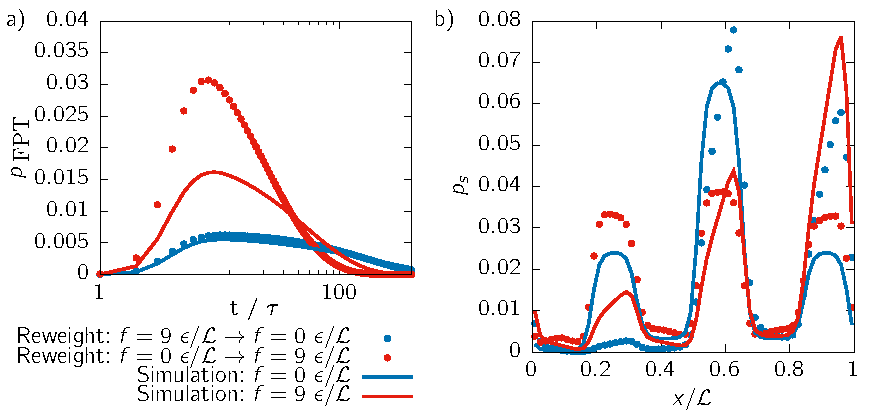
\includegraphics{../plots/Jaynes/fpt_J_2010_2910.pdf}
 % fpt_J_2010_2910.pdf: 0x0 px, 300dpi, 0.00x0.00 cm, bb=
 \caption[Stationary distribution and first-passage time distribution for the driven 1D system reweighted with respect to global entropy production.]{Comparing (a) the stationary distribution $p_s$ and (b) the FPTD $p_{\; \text{FPT}}$ for the process $B \rightarrow C$ of the equilibrium system ($f=0~\epsilon / \mathcal{L}$) and driven system ($f=9~\epsilon / \mathcal{L}$). The reweighting procedure tests the global entropy production of the target system as a defining system constraint.}
 \label{fig:rewtrial1}
\end{figure}
\subsubsection{Local Entropy Production}
Enforcing the local entropy production requires a Lagrangian multiplier at each transition. Determining a value for each transition means to couple the same reservoir at a different strength. 
The Caliber is defined by
 \begin{equation}
\begin{aligned}
 \mathcal{C}_{\Delta S_{ij}} &= -\sum_{i,j} \pi_i p_{ij} \ln \frac{p_{ij}}{q_{ij}} 
      +  \sum_i \mu_i \pi_i \left( \sum_j p_{ij} - 1 \right) + \zeta \sum_i ( \pi_i -1) \\
    &+ \sum_{i,j} \pi_i \alpha_{ij} \left ( \ln \frac{p_{ij}}{p_{ji}} -  \Delta S_{ij}  \right ),
\end{aligned}
\end{equation}
using the local entropy production relating the forward and backward 
jumping probability (see section~\ref{sec:NESS}). The Lagrangian multiplier $\alpha_{ij}$ and $\mu_i$ were rescaled by $\pi_i$.   
The maximisation with respect to the transition probabilities gives
  \begin{equation}
    0 = - \pi_i \ln \left ( \frac{p_{ij}}{q_{ji}} \right ) - \pi_i + \pi_i     \mu_i + \pi_i \frac{ \alpha_{ij} }{p_{ij}} - \pi_j \frac{ \alpha_{ji} }{p_{ij}}.
  \end{equation}
Solving for $p_{ij}$ with $\pi_i \neq 0$ 
  \begin{equation}
  p_{ij} = q_{ij} \; \exp \left ( -1 + \mu_i  + \frac{\gamma_{ij}}{p_{ij}} \right ),
\label{eq:pijearly}
  \end{equation}
where $\gamma_{ij} = \alpha_{ij} - \frac{\pi_j}{\pi_i} \alpha_{ji}$ is used.
Enforcing the local entropy productions explicitly by $\Delta S_{ij} = \ln \frac{p_{ij}}{p_{ji}}$ and after some algebra one finds
\begin{equation}
 \frac{\gamma_{ij}}{p_{ij}} = w_{ij} \left ( \Delta S_{ij} - \Delta S_{ij}^q -\mu_i + \mu_j \right ),
\end{equation}
where the definitions $w_{ij} = 1/\left(1 + \frac{\pi_i p_{ij}}{\pi_j p_{ji}} ) \right)$ and 
$\Delta S_{ij}^q = \ln \frac{q_{ij}}{q_{ji}} $ have been used. This expression is plugged into equation \ref{eq:pijearly} and using $w_{ij} + w_{ji} =1$ we  find
\begin{equation}
 p_{ij} = q_{ij} \exp \left ( -1 + w_{ji} \mu_i + w_{ij} \mu_j + w_{ij} (\Delta S_{ij} -\Delta S_{ij}^q)  \right ) 
\label{eq:pij2early}
\end{equation}
The Caliber maximisation with respect to the stationary distribution gives
  \begin{equation}
    \begin{aligned}
      0 =& -\sum_k p_{ik} \ln \left ( \frac{p_{ik}}{q_{ik}}  \right ) + \mu_i \sum_k p_{ik} - \mu_i  +\zeta  \\
      &+ \sum_{k} \alpha_{ik} \left( \ln \left ( \frac{p_{ik}}{p_{ki}} 
\right) - \Delta S_{ik}  \right  ) .
    \end{aligned}
  \end{equation}
  By plugging in equation \ref{eq:pijearly} and making use of the constraints, one finds a relation between the $\gamma_{ij}$ and $\mu_i$:
  \begin{equation}
    \mu_i  = 1 + \zeta + \sum_k \gamma_{ik}.
  \end{equation}
Defining $c_i = \sum_k \gamma_{ik} $ and plugging $\mu_i$ into equation \ref{eq:pij2early}
 results in the final equation
 \begin{equation}
 p_{ij} = q_{ij} \exp \left ( \zeta + w_{ji} c_i + w_{ij} c_j + w_{ij} (\Delta S_{ij} -\Delta S_{ij}^q)  \right ).
 \label{eq:altpij}
 \end{equation}  
The constraint of conserved transition probabilities $\sum_k p_{ik} =1 $ gives
 \begin{equation}
 1 = \sum_k q_{ik} \exp \left ( \zeta + w_{ki} c_i + w_{ik} c_k + w_{ik} (\Delta S_{ik} -\Delta S_{ik}^q)  \right ).
 \end{equation}
 This equation can be solved for $\bm{c}$ by  numerical iteration, discussed in the following section \ref{sec:numerics}.
 The result of enforcing local entropy productions is shown in figure \ref{fig:rewtrial2}. The stationary distribution is reproduced correctly by the reweighting procedure, showing a significant improvement compared to the global constraint. The dynamics are not reproduced correctly, indicating that the current model of a reservoir providing heat locally is not sufficient. 
 
  \begin{figure}[t]
 \centering
 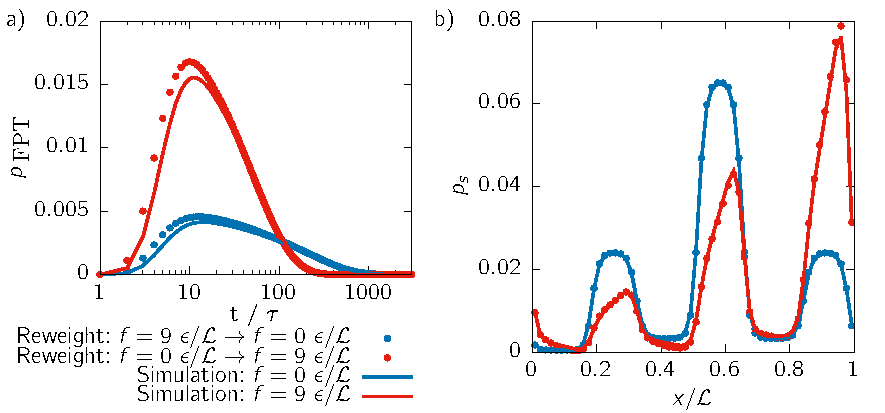
\includegraphics{../plots/Jaynes/fpt_Sloc_2010_2910.pdf}
 % fpt_J_2010_2910.pdf: 0x0 px, 300dpi, 0.00x0.00 cm, bb=
 \caption[Stationary distribution and first-passage time distribution for the driven 1D system reweighted with respect to local entropy production.]{Comparing (a) the stationary distribution $p_s$ and (b) the FPTD $p_{\; \text{FPT}}$ for the process $B \rightarrow C$ of the equilibrium system ($f=0~\epsilon / \mathcal{L}$) and driven system ($f=9~\epsilon / \mathcal{L}$). The reweighting procedure tests local entropy productions of the target system as a defining system constraint.}
 \label{fig:rewtrial2}
\end{figure}
\subsubsection{Local Entropy Production and Global Balance}
The previous constraints define the interaction on every transition with the reservoir but the influence of local changes on the whole system are not modelled. We add global balance $\pi_i = \sum_k \pi_k p_{ki} \; \forall i$ as a condition for NESS (see section~\ref{sec:NESS}) to the list of constraints. It connects a single state on the left-hand side of the equation to all other states of the global system on the right-hand side. Furthermore, it builds a connection between stationary and dynamic probabilities that were previously maximised without specific coupling. The full Caliber is given by
  \begin{equation}
    \begin{aligned}
      \mathcal{C} = -&\sum_{i,j} \pi_i p_{ij}\ln \frac{p_{ij}}{q_{ij}} 
      +   \sum_i \mu_i \pi_i \left( \sum_j p_{ij} - 1 \right) + \zeta ( \sum_i \pi_i -1) \\
      +&  \sum_j \pi_j \nu_j \left(\sum_i \pi_i p_{ij} - \pi_j \right) 
      + \sum_{ij} \pi_i  \alpha_{ij} \left( \ln \left( 
\frac{p_{ij}}{p_{ji}} \right) - \Delta S_{ij} \right).
    \end{aligned}
  \end{equation}
The maximisation is performed equivalently to the derivation without global balance, just with additional Lagrangian multiplier $\nu_i$. The maximisation with respect to transition probabilities equivalent to equation \ref{eq:pijearly} becomes
  \begin{equation}
  p_{ij} = q_{ij} \; \exp \left ( -1 + \mu_i + \nu_j + \frac{ \gamma_{ij} 
}{p_{ij}} \right ).
  \label{eq:pij}
  \end{equation}
The maximisation of the Caliber with respect to the stationary distribution 
shows
  \begin{equation}
    \begin{aligned}
      0 =& -\sum_k p_{ik} \ln \left ( \frac{p_{ik}}{q_{ik}}  \right ) + \mu_i 
\sum_k p_{ik} - \mu_i \\& +\zeta + \sum_k \nu_k p_{ik} - \nu_i 
      + \sum_{k} \alpha_{ik} \left( \ln \left ( \frac{p_{ik}}{p_{ki}} 
\right) - \Delta S_{ik}  \right  ) .
      %\\ & + \gamma \sum_k p_{ik} F_{ik} 
    \end{aligned}
  \end{equation}
  By making use of the constraint $\sum_k p_{ik}=1$ and equation \ref{eq:pij} one finds a relation between the Lagrangian multipliers $\gamma_{ij} = \alpha_{ij} - \frac{\pi_j}{\pi_i} \alpha_{ji}$, $\mu_i$ and $\nu_i$:
  \begin{equation}
    \mu_i + \nu_i = 1 + \zeta + \sum_k  \gamma_{ik}
  \label{eq:minpi}
  \end{equation}
  Making use of equation \ref{eq:pij} to enforce the local entropy productions $\Delta S_{ij} = \ln \frac{p_{ij}}{p_{ji}}$, where $\Delta S_{ij}^q = \ln \frac{ q_{ij}}{q_{ji}}$ denotes the reference entropy production and the definition $w_{ij} = 1/\left(1 + \frac{\pi_i p_{ij}}{\pi_j p_{ji}} ) \right)$ is used again
    \begin{equation}
    \frac{ \gamma_{ij}}{p_{ij}} = w_{ij} \left ( \Delta S_{ij} - \Delta 
S_{ij}^q -\mu_i +\mu_j -\nu_j +\nu_i \right ).
      \label{eq:alpha}
    \end{equation}
Plugging this result into equation \ref{eq:pij} gives
\begin{equation}
  p_{ij} = q_{ij} \; \exp \left ( -1 + w_{ji} \mu_i + w_{ij} \mu_j 
  + w_{ji} \nu_j + w_{ij} \nu_i + w_{ij} ( \Delta S_{ij} - \Delta S_{ij}^q )  \right ) . 
\label{eq:pij2}
\end{equation}
Enforcing the constraint $\sum_k p_{ik} =1 $ results in a set of 
N equations, where $N$ is the number of microstates. Combined with equations~\ref{eq:minpi} there is a set of $2N$ non-linear equation to be solved.
 \begin{figure}[t]
 \centering
 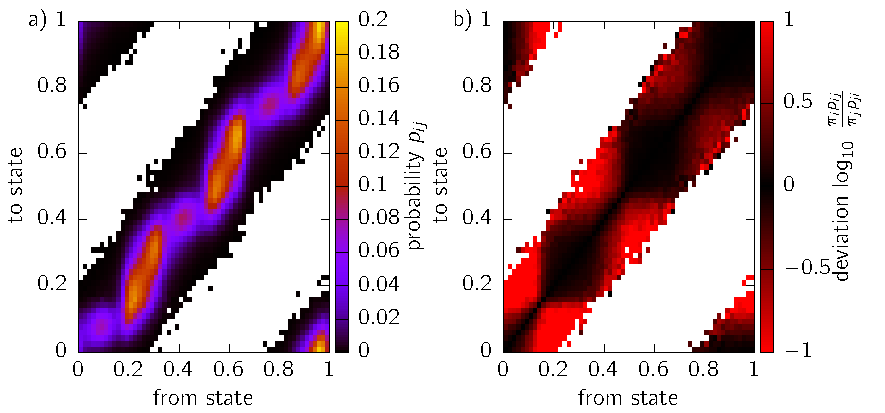
\includegraphics{../plots/Jaynes/ratio_all.pdf}
 % fpt_J_2010_2910.pdf: 0x0 px, 300dpi, 0.00x0.00 cm, bb=
 \caption[Transition probability matrix of the 1D driven system and the violation of detailed balance.]{(a) the transition probabilities for the driven system ($f=9~\epsilon / \mathcal{L}$). (b) the deviation from detailed balance in the form $\log_{10} \frac{\pi_i p_{ij}}{\pi_j p_{ji}}$. The black regions around $0$ indicate that detailed balance holds approximately, red regions indicate violation of detailed balance. The matrix is antisymmetric by definition.}
 \label{fig:Sprod}
\end{figure}
In order to do that, we approximate that the deviation from detailed balance is small. Mathematically we assume that $\frac{\pi_i p_{ij}}{\pi_j p_{ji}} \approx 1 $, resulting in $w_{ij} \approx \frac{1}{2}$.  The approximation close to detailed balance is applied for a single Markovian jump --- a trajectory consists of many jumps and can grow large entropy productions despite the approximation. 
Figure~\ref{fig:Sprod} illustrates that this is a reasonable approximation for the important transitions where $p_{ij}$ is large.  
\begin{figure}[t]
 \centering
 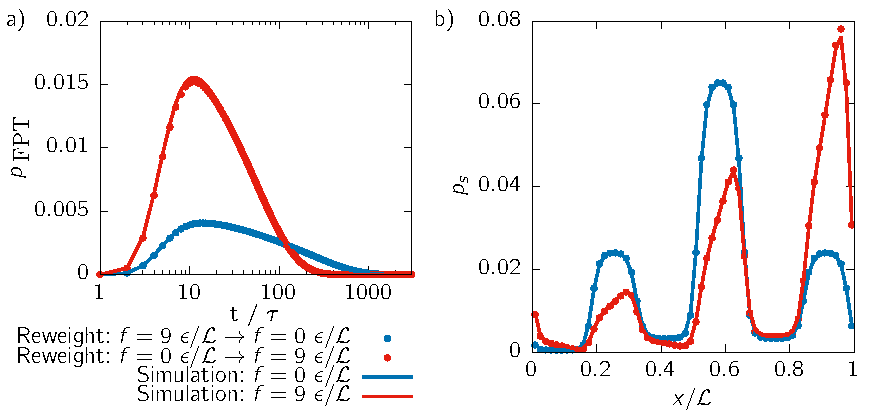
\includegraphics{../plots/Jaynes/fpt_2010_2910.pdf}
 % fpt_J_2010_2910.pdf: 0x0 px, 300dpi, 0.00x0.00 cm, bb=
 \caption[Stationary distribution and first-passage time distribution for the driven 1D system reweighted with respect to local entropy production and global balance.]{Comparing (a) the stationary distribution $p_s$ and (b) the FPTD $p_{\; \text{FPT}}$ for the process $B \rightarrow C$ of the equilibrium system ($f=0~\epsilon / \mathcal{L}$) and driven system ($f=9~\epsilon / \mathcal{L}$). The reweighting procedure with local entropy production of the target system and global balance  recovers dynamics and statics well.}
 \label{fig:rewtrial3}
\end{figure}
Using the approximation on equation \ref{eq:pij2} gives
    \begin{equation}
      p_{ij} = q_{ij} \exp \left ( \frac{1}{2} \left ( -2 + \mu_i +\nu_j +\mu_j 
+ \nu_i + \Delta S_{ij} - \Delta S_{ij}^q \right ) \right ).
    \end{equation}
    Using the result of equation \ref{eq:minpi} and the definition $c_i = \sum_k \gamma_{ik}$ shows
    \begin{equation}
    \begin{aligned}
    p_{ij} =& q_{ij} \exp \left ( \zeta+ \frac{1}{2} \left ( c_i + c_j + \Delta
S_{ij} - \Delta S_{ij}^q \right ) \right ) \\
=&     \sqrt{q_{ij} q_{ji} } \exp \left ( \zeta+ \frac{1}{2} \left ( c_i + c_j + \Delta
S_{ij} \right ) \right ). 
    \end{aligned}
    \label{eq:finalpij}
    \end{equation}
This shows that we have two options for the input parameters: The reweighting depends either on the total entropy production of the target system or the difference in local entropy production of target and reference system. 
The unknowns $\bm{c}$ are calculated by enforcing the relation 
$\sum_j p_{ij} =1 $
    \begin{equation}
      1 = \sum_j q_{ij} \exp \left ( \zeta+ \frac{1}{2} \left ( c_i + c_j + \Delta 
S_{ij} - \Delta S_{ij}^q \right ) \right ),
      \label{eq:iteration}
    \end{equation}
being a non-linear system of equations that can be solved numerically. It will be shown in section \ref{sec:numerics} that this set of equations in convex and has a unique solution, independent of initial conditions on the solving algorithm. $\zeta$ is a Lagrangian multiplier that can be set to $0$ because the corresponding constraint $\sum_k \pi_k = 1$ is implicitly met by the rowwise normalisation of the transition matrix and 
its enforced relation to the stationary distribution by global balance 
$\pi_i = \sum_k \pi_k p_{ki}$.  The results of the reweighting procedure,using the approximated solution is given in figure \ref{fig:rewtrial3}. Both quantities are estimated correctly reweighted from equilibrium to off-equilibrium and vice versa, indicating that the combination of local entropy production and global balance as constraint apply for this system. 

The outcome of the Caliber maximisation without global balance in equation \ref{eq:altpij} is equivalent to the final equation \ref{eq:finalpij} when the same approximation $w_{ij} \approx \frac{1}{2}$ is applied. It  can thus not be argued that the global balance condition is indeed essential for the reweighting process, but we can argue that local entropy productions alone are not sufficient. It is possible that another constraint, which could not be identified, leads to equation \ref{eq:finalpij} without approximation. A possible candidate is a reservoir not connected to the transition, but to the single states of the system. An indicator are the responsible $N^2$ Lagrangian multipliers $\alpha_{ij}$ not being calculated in the maximisation because they are reduced to the $N$ parameters $c_i$. It follows that only the strength of coupling to each state is calculated separately.

We will stick to to the given equation for this thesis because it produces excellent, fast and unique results for different systems. The presented set of non-linear equations without approximation may not have a unique solution and is too complex for fast application. The  enforced constraints on the entropy production hold true with a relative error less than $ 10^{-9}$, 
indicating the approximation applies for the given system. This test can be run for every system the algorithm is applied to.  However, a full solution in agreement with the approximated form would prove that global balance is essential for reweighting. It would also give mathematical ground to apply the reweighting procedure to systems under stronger driving.  


\subsection{Invariant Measure}
\label{sec:Invariant}
Reweighting suggests that there is an underlying quantity that is the same for all systems. For Equilibrium systems, it is the density of states. Once it is known one can construct the system at any thermodynamic point, because the quantity is independent of the ensemble and the microstate weigthing of the ensembles is known. For the current reweighting scheme, we expect an underlying invariant too. It does not have to be completely independent of thermodynamics, only of the quantities that are altered by reweighting. The temperature for instance is constant for all systems.

Starting with the reweighting formulae in equation~\ref{eq:finalpij}, the product of forward and backward transition is denoted by
  \begin{equation}
    p_{ij} p_{ji} = q_{ij} q_{ji} \exp ( c_i + c_j + 2 \zeta ),
    \label{eq:pp}
  \end{equation}
where the symmetry of local entropy production is used to cancel $\Delta S_{ij} =- \Delta S_{ji}$. Similarly, we may reweight the other way round from $q_{ij}$ to $p_{ij}$ with another set of constants $\mathbf{\tilde c}$:
  \begin{equation}
    q_{ij} q_{ji} = p_{ij} p_{ji} \exp ( \tilde c_i + \tilde c_j + 2 \tilde 
\zeta  ) .
    \label{eq:qq}
  \end{equation}
  Combing both equation~\ref{eq:pp} and \ref{eq:qq} results in:
  \begin{equation}
    - \tilde c_i - \tilde c_j - 2 \tilde \zeta = c_i + c_j + 2 \zeta.
  \end{equation}
Using this result to plug into equation~\ref{eq:pp}, the expression 
  \begin{equation}
    I_{ij}^2 = p_{ij} p_{ji} \exp \left ( \frac{\tilde c_i + \tilde c_j}{2} +\tilde 
\zeta \right ) 
= q_{ij} q_{ji} \exp\left ( \frac{ c_i + c_j}{2}+ \zeta \right )
  \end{equation}
is invariant under reweighting. It is constant under different driving of the  system. Note that $I_{ij}$ is defined up to a constant $\zeta$. This quantity and its physical meaning will be discussed in detail in section~\ref{sec:InvariantC}. 
 
\subsection{Numerical Maximisation}
\label{sec:numerics}
For an exact solution of the set of $2N$ equations 
\begin{equation}
 \begin{aligned}
 0 &=\sum_k^N q_{ik} \; \exp \left ( -1 + w_{ik} \mu_k + w_{ki} \mu_i 
  + w_{ik} \nu_i + w_{ki} \nu_k + w_{ik} ( \Delta S_{ik} - \Delta S_{ik}^q )  \right )  \\
0&= - \mu_i - \nu_i + 1 + \zeta + \sum_k^N p_{ik} w_{ik} \left ( \Delta S_{ik} - \Delta S_{ik}^q -\mu_i +\mu_k -\nu_k +\nu_i \right )    
 \end{aligned}
\label{eq:fullsol}
\end{equation}
has to be solved for the Lagrangian multiplier vectors $\bm{\mu}$ and $\bm{\nu}$. The Kullback-Leibler divergence alone is a convex function, but constraining to the non-linear local entropy production introduced non-convexity. It is not a priori known if there is a unique solution of the equations. Finding an analytic solution failed, so we solve it by numerical methods. 

The analytic solution expanded $w_{ij} = 1/\left(1 + \frac{\pi_i p_{ij}}{\pi_j p_{ji}} ) \right)$ around detailed balance. It will be shown in the following that the resulting set of equations becomes convex and possible solutions for higher order expansion will be suggested.  


\subsubsection{0th Order Expansion}
The system of equations \ref{eq:iteration} resulting from the 0th order expansion are rewritten by the definitions $\Phi_i = \exp (c_i/2 )$ and $A_{ij} = q_{ij}\exp \left ( \zeta+ \frac{1}{2} \left (  \Delta S_{ij} - \Delta S_{ij}^q \right ) \right )$. 
The equations \ref{eq:iteration} become 
\begin{equation}
  \Phi_i = \frac{1}{\sum_k A_{ik} \Phi_k}.
\end{equation}
We define this function as $f_i= \Phi_i$ and show that it is convex by calculating the Hessian
\begin{equation}
    \frac{\partial^2 f}{ \partial \Phi_m \partial \Phi_n} =  \frac{2 A_{im} 
A_{in}}{\left ( \sum_k A_{ik} \Phi_k \right )^3}.
\end{equation}
Noting that $\Phi_i  \geq 0$ and $A_{ij} \geq 0$, the Hessian is 
positive definite and the function is convex. This means that a random starting point for $\Phi_i^{(0)}> 0$  can be chosen to find a numerical solution to this problem. We found that the least squared method with the implementation in pythons library \lstinline{scipy.optimize.least_squares}~\cite{branch1999subspace} and $\Phi_i\geq 0$ bounded below  gives the most robust result. 

\subsubsection{Full Solution}
We briefly show why the approximated solution is used throughout the thesis by attempting to solve the exact set of equation. The methods are applied to the testing system with 30 microstates by reweighting equilibrium data to itself.  We tried different numerical methods provided by scipy including:
\begin{itemize}
 \item Root finder (\lstinline{scipy.optimize.fsolve}~\cite{more1980user},
 \lstinline{scipy.optimize.least_squares}~\cite{branch1999subspace})
 \item Function minimiser (\lstinline{scipy.optimize.minimize(method="L-BFGS-B")}~\cite{zhu1997algorithm})
 \item Basinhopping (\lstinline{scipy.optimize.basinhopping}~\cite{wales1997global})
\end{itemize}
The root finding method uses the equations~\ref{eq:fullsol} directly and solves the set of equations self-consistently until a root is found, similar to the self-iteration. The other two methods need an error function $\mathcal{E} = \sum_i^N g_i f_i$ for numerical minimisation, where $f_i$ represents one equation in \ref{eq:fullsol} and $g_i$ weights each function. All methods need an initial point to start the algorithm.  As discussed earlier, the functions are non-convex and may have more than one minimum. The basinhopping algorithm attempts to solve this problem by using random displacements of parameters followed by error-function minimisation. The algorithm combines multiple minimisations but is not guaranteed to find the global minimum. The prospect is better because the method becomes less dependent on its initial value for long runtime. 

The parameters $w_{ij}$ depend on the stationary distribution $\bm{\pi}$ of the target system. We use the stationary algorithm of the 0th-order approximation to estimate $\bm{\pi}$ as it shows excellent agreement with the values known from simulation for the testing system. In a general application, one could add 
the linear dependence $\sum_k \pi_k p_{ik} = \pi_i$ to the list of equations but this is set aside for now. Applying the algorithm to the original set of equations we find that the variables tend to diverge. This problem is solved by the transformation
\begin{equation}
 \begin{aligned}
  u_i &= \mu_i - \nu_i \\
  v_i &= \mu_i + \nu_i
 \end{aligned}
\end{equation}
resulting in the new set of equations
\begin{equation}
\begin{aligned}
0 &= \sum_k q_{ik} \exp \left ( -1 + \frac{1}{2} \left( v_i + v_k +u_i -u_k \right ) + w_{ik} \left( -u_i + u_k + \Delta S_{ik} - \Delta S^q_{ik} \right) \right ) \\
0 &= 1 + \zeta -v_i + \sum_k p_{ik} w_{ik} \left ( \Delta S_{ik} - \Delta S^q_{ik}  -u_i +u_k \right ) .
\end{aligned}
\label{eq:fullsolTra}
\end{equation}
Comparing these equations to the approximated solution using $w_{ij}\approx \frac{1}{2}$ in equation~\ref{eq:iteration} shows that $\bm{v}$ takes the role of $\bm{c}$, and $\bm{u}$ are the new set of constants. This provides a starting point for the iteration at $\bm{v}= \bm{c}$,  $\bm{u}=0$ and $\zeta =0$.  Note that this choice does satisfy the first set of equations~\ref{eq:fullsolTra} for reweighting in equilibrium (i.e. $w_{ij} = \frac{1}{2}$) but not the second set of equations. 

The transformation solves the problem of diverging variables but reveals that the algorithms are unable to find a solution that fulfils all constraints. The root-finding methods fail to converge. The minimisation methods reveal that most constraints are fulfilled but there are large local errors as shown in figure~\ref{fig:fullsol}. The location of these errors can be changed by reassigning weighting factors $g_i$ of the error function $\mathcal{E}$. The basinhopping algorithm can find solutions with lower error but non with error vanishing for a complete solution. 

 \begin{figure}[t]
 \centering
 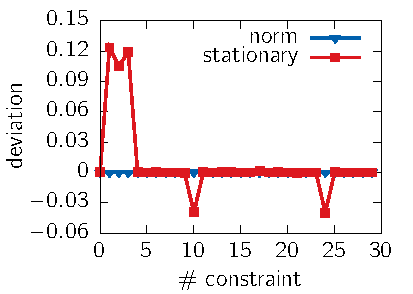
\includegraphics{../plots/Jaynes/fullsol.pdf}
 % fpt_J_2010_2910.pdf: 0x0 px, 300dpi, 0.00x0.00 cm, bb=
 \caption[Deviation of constraints when attempting to find a full solution to the Caliber maximisation by numerical minimisation.]{Deviation of constraints solving the full set of equations~\ref{eq:fullsolTra}. \enquote{Norm} refers to the first set of equation, \enquote{stationary} to the second.  }
 \label{fig:fullsol}
\end{figure}


Since finding a full solution is burdensome, we attempt to find solutions for higher order expansions. Expanding $w(x)$ where $x=\frac{\pi_i p_{ij}}{\pi_j p_{ji}} $ around 1 for the higher orders gives
\begin{equation}
 w(x) \approx \frac{1}{2} - \frac{x}{4} +\frac{x^3}{48} + \text{h.o.}.
\end{equation}
The same initial values as for the attempt of full solution $\bm{v}= \bm{c}$, $\bm{u}=0$ and $\zeta =0$ are chosen. The idea is based on solving the system approximately for the 1st-order approximation, use the output for an initial guess on the 3rd order approximation and continue until a full solution is found. In practice this attempt suffers from local errors like the full solution. 

The above discussion indicates that a full solution is difficult to find or not existent. In either case, the solution given by the 0th order expansion shows excellent results and will be used throughout the paper. Finding a full solution is nevertheless desirable. If the full solution can be shown to be exact in the sense of reweighting data, it indicates that the global balance condition completes the set of constraint for a NESS.

%  
% \bibliography{/home/marius/PhD/Thesis/references.bib}
% \bibliographystyle{plain}
% \end{document}
% 
% 
% 
% 


















% 
% %\documentclass[paper=a4,fontsize=12pt,open=right,noabbrev]{report}
% \documentclass[12pt]{report}
% \usepackage[utf8]{inputenc}
% \usepackage{amsmath}
% \usepackage{amssymb}
% \usepackage{graphicx}
% \usepackage{placeins}
% \usepackage{cite}
% \usepackage{physics}
% \usepackage{mathrsfs}
% \usepackage{geometry}
% % \usepackage{layouts}
% \usepackage{newfloat}
%  \usepackage{float}
% 
% \setlength{\parindent}{0em}
% \setlength{\parskip}{1em}
% 
% 
% %% Technical point floatstyle
% \floatstyle{ruled}
% \newfloat{Technical Point}{htbp}{lop}[chapter]
% 
% 
% \begin{document}

\chapter{Reweighting Dynamics in full Conformational Space }
\label{ch:RewU}

 
This chapter focuses on testing the reweighting scheme introduced in section~\ref{sec:RewOffEqu} on minimal models where the full conformational space is known. We have seen in chapter~\ref{ch:Jaynes} that the chosen set of constraints apply for a test model. We extend this testing by variation of of  potentials, dimension and magnitude of local and global forces. The models consist of a single particle so entropic effects due to many-body interactions are absent. This provides a minimal testing ground for the reweighting method based on the Maximum Caliber. At first, an equilibrium model with changing potential surface is test for the special case of equilibrium systems. The second systems extends to non-equilibrium steady states (NESS) by a global external force with periodic boundary conditions, introduced in section~\ref{sec:1Dmodel}. The third system is inspired by a laser model and pushes the system in a NESS by applying non-conservative forces locally~\cite{khan1983mechanism}. The last model adds one dimension and tests the global driving on a 2-dimensional single particle. 

The systems are simulated using molecular dynamics for 10 different driving forces and a Markov State Model (MSM) is constructed. One system is reweighted continuously to other thermodynamic state points and checked if dynamical and static information from simulation are recovered correctly. The static information is tested using the stationary distribution, the dynamical information is tested using the first-passage-time distribution (FPTD) between metastable states (see section~\ref{sec:FPTD}). Selected processes are compared by full FPTD, because comparison of all FPTD with each other is cumbersome. The systems are compared by the first three moments of the FPTD and the metastable state occupation probabilities $\Pi$. The reweighting test is considered successful if all information is recovered correctly.

The presented results for all models except the 2D model were published in~\cite{bause2019microscopic}.


\section{Single Particle in 1D Potential Well}
\label{sec:equ}
\begin{figure}[h]
\centering
 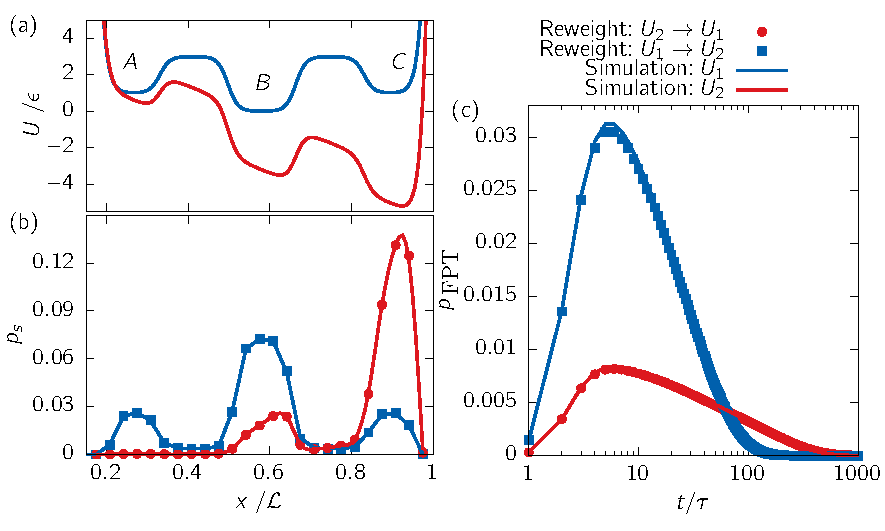
\includegraphics{../plots/Urew/single_3003.pdf}
 \caption[Potential surface, stationary distribution and first-passage time distribution of a chosen process for the 1D equilibrium system]{ (a) Potential, (b) stationary distribution and (c) FPTD of the process $ C \rightarrow B$. The lines in (b,c) represent the results from simulating the system potentials, the dots are the results from reweighting the systems into each other. $A$, $B$, $C$ mark the metastable states. The system without tilting is represented blue, the system with tilting in red. }
 \label{fig:potequ} 
\end{figure}

The reweighting procedure is designed for general NESS. We will test it on the special case of an equilibrium model first. The potential shown in figure~\ref{fig:potequ} is a 1D potential of a type presented in section~\ref{sec:1Dmodel} with diverging boundaries and three potential wells. 
The applied force in positive direction can be described by an additional potential $U_{\text{ext}}(x) = -f x $ that tilts the existing potential. The diverging boundaries prevent the system to enter a NESS and restrict the system to equilibrium. Equilibrium is a case of a NESS without entropy production on average and the dynamics are governed by detailed balance. It ensures that the heat dissipated moving a particle between two points in space does not depend on the chosen trajectory. The MSM was constructed with a lagtime $0.004\,\mathcal{T}$ and $60$ microstates. 
 
The static and dynamic properties for the system without potential tilt and with maximum tilting at $f= 9\,\frac{\epsilon}{\mathcal{L}}$ are shown in figure~\ref{fig:potequ}. The presented FPTD from state $C$ to $B$ slows down significantly with increasing tilting. Transition times above $50\,\tau$ are rare in the reference system and become likely in the new potential. The reweighting procedure recovers this detailed view on the dynamics. Previously unknown trajectories are captured by the reweighting correctly. 
\begin{figure}
\centering
 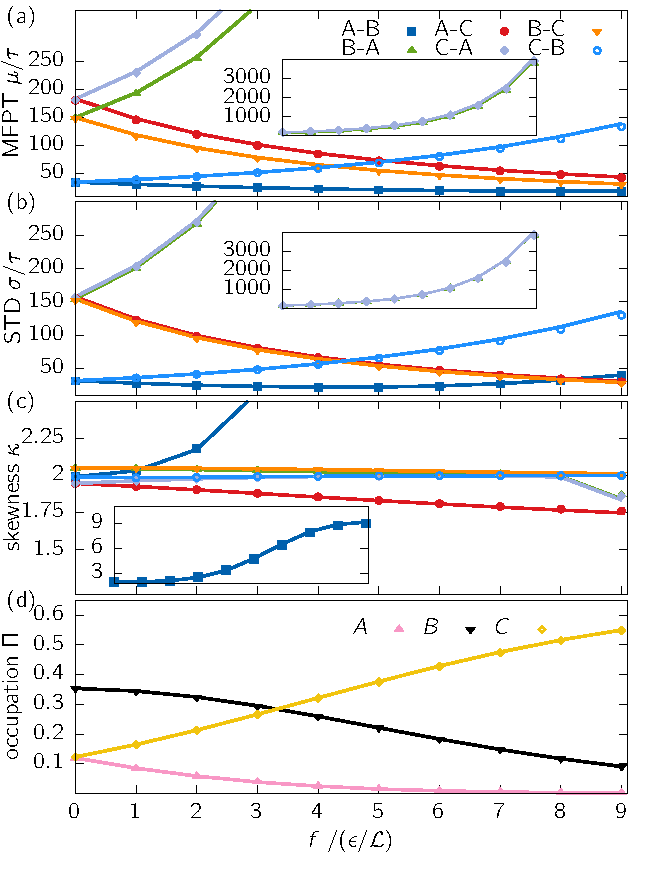
\includegraphics{../plots/Urew/mom_3003.pdf}
 \caption[The first three moments and the population of metastable states for the equilibrium system under varying tilt of the potential.]{$(a-c)$ The first three moments of the FPTD for all six processes between metastable states in figure~\ref{fig:potequ}a under varying tilting of the potential. $(d)$ The occupation probability of each metastable state. The dots represent the value measured from simulation. The line is the equilibrium system continuously reweighted.  }
 \label{fig:momequ}
\end{figure}

Figure~\ref{fig:momequ} presents the first three moments and the occupation probability of the metastable states. The potential is constructed such that two processes have the same FPTD in equilibrium: $A \rightarrow B$ and $C \rightarrow B$ going from left and right inwards to the central potential, their inverse processes going outwards from the central potential and processes $A \rightarrow C$ and $C \rightarrow A$. The latter processes  crossing the whole system via state $B$ and can be seen as a combination of two processes. The additional force breaks the symmetry and speeds up the processes in the direction of the force, while inverse processes are slowed down. The standard deviation (STD) of the distributions show the same behavior as the mean first-passage time (MFPT). A larger mean allows larger variation. The skewness is  stable at $\approx 2 $, except for the process $A \rightarrow B$. This process is increasingly fast, such that it is described by processes of time-length of the lagtime $\tau$, as shown in figure~\ref{fig:potequ}c. The fast processes cannot be described in all detail anymore, resulting in a tilting of the distribution and an increasing skewness. Smaller lagtime of the MSM would shift this effect to higher driving forces.  

Reweighting continuously from the equilibrium system shows the precision of the method over the range of driving forces. Furthermore, the driven states between the simulated ones can be explored without additional simulation. It is concluded that the reweighting method recovers static and dynamic properties from reweighting for the special case of equilibrium systems. We will turn to the general class of all NESS in the next section.



\FloatBarrier
\section{Single Particle in 1D under Global Driving}
\label{sec:1gl}
\begin{figure}[h]
 \centering
 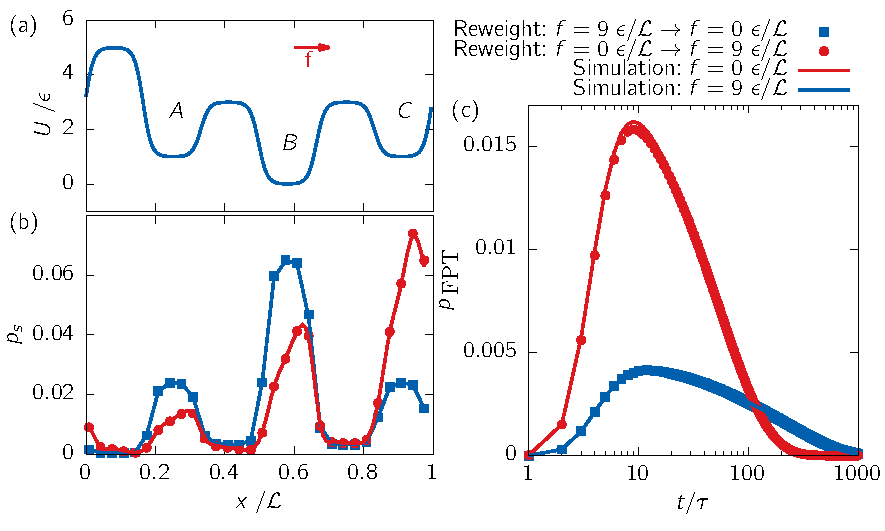
\includegraphics{../plots/Urew/single_2010.pdf}
 \caption[Potential surface, stationary distribution and first-passage time distribution of a chosen process for the 1D driven system]{ (a) Potential and external force (b) stationary distribution and (c) FPTD of the process $ C \rightarrow B$. The lines in (b,c) represent the results from simulating a single particle in the potential without (blue) and with (red) external force. The dots are the results from reweighting the systems into each other. $A$, $B$, $C$ mark the metastable states. }
 \label{fig:potgl}
\end{figure}

A single particle in 1D periodic-boundary potential is driven in one direction by an external force. Since the particle has a preferred direction to move the dynamics do not fulfil detailed balance. The external force cannot be described by a potential. The heat dissipated to move the particle between two space-points becomes path-dependent. In particular, the heat  dissipated depends on weather the particle moving between two points in space along a trajectory with or against the external force. The present model is a minimal example to describe a NESS. The reweighting scheme will be shown to capture the path-dependence of the dynamics correctly.

The corresponding MSM describing the dynamics is constructed from simulation data in detail in section~\ref{sec:MSM} with a lagtime $\tau = 0.002\,\mathcal{T}$ and $60$ microstates. The reference potential surface with non-conservative forces is shown in figure~\ref{fig:potgl}a. The diverging potential at the boundaries of the equilibrium system in the previous section~\ref{sec:equ} was replaced  by a potential barrier of height $5\,\epsilon$. The stationary distribution and a FPTD for a chosen process without driving and a system driven by $9\, \frac{\epsilon}{\mathcal{L}}$ are shown in figure~\ref{fig:potgl}b,c. The systems are reweighted into each other. The simulation and reweighting data match precisely for the stationary distribution and the FPTD from state $C$ to $B$. 

\begin{figure}[t]
\centering
 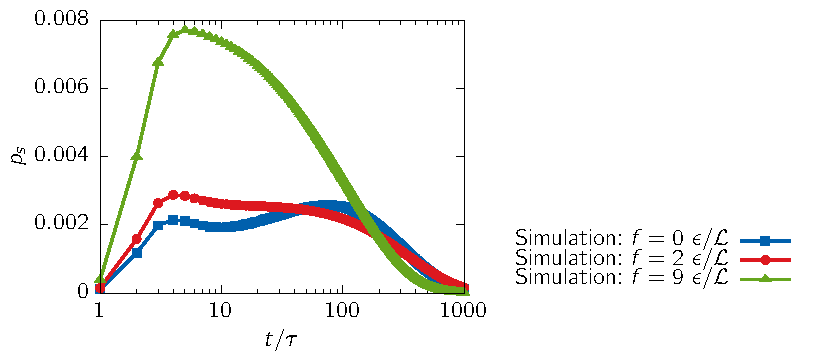
\includegraphics{../plots/Urew/fpt_2010.pdf}
 \caption[First-passage time distribution of transition $C\rightarrow A$ simulated at 3 different driving forces for the 1D driven system.]{FPTD of transition $C\rightarrow A$ simulated at 3 different driving forces. The equilibrium system at $f=0$ is a bimodal distribution, indicating two sets of trajectories for that trajectory. The two peaks merge to one as driving increases. One set of trajectories is suppressed by the driving.  }
 \label{fig:fpt1D}
\end{figure}

The potential shown in figure~\ref{fig:potgl}a represents the equilibrium system without driving force.  The direction of the force is marked in red and applied over the whole system with equal strength. The first three moments of the FPTD for all involved slow processes and the stationary distribution of metastable states is shown in figure~\ref{fig:momgl}. The processes $A\rightarrow B$ and $B\rightarrow C$ are aligned with the external force and become faster. The process $C\rightarrow A$ shows abnormal behaviour by slowing down first and speeding up at force $> 4\,\frac{\epsilon}{\mathcal{L}}$. For the reference system, the connection via state $B$ is spatially longer but more probable than the direct connection over the large barrier. Both sets of trajectories are presented by two peaks in the FPTD in figure~\ref{fig:fpt1D}. This weighting of path changes under driving until the jump over the large barrier between the states becomes more probable for increasing driving. At this point, the process speeds up with increasing force. The process $B\rightarrow A$ opposing the external force slows down first. After the jump over the barrier between state $A$ and $C$ becomes more probable, the transition  $B\rightarrow A$ benefits from using new transition trajectories via state C and increases speed. The transition $C\rightarrow B$ slows down against the force. We can expect that the trend changes for larger forces too.  The STD show a similar behaviour as the MFPT as seen for the previous system. The skewness is more variable, but stays in a range of $\approx 2 $. The skewness of transition $A\rightarrow B$ increases due to its strong increase in short-term processes, as described for the previous system in section~\ref{sec:equ}. The increase is less than for the previous system, because a lower lagtime for the MSM was chosen. The occupation probability changes over driving such that state $B$ becomes higher populated than state $C$ for driving $> 4\,\frac{\epsilon}{\mathcal{L}}$. This \textit{population inversion} is an off-equilibrium effect where population of high energy states is larger than the population of low energy states~\cite{maes2018non}. It cannot exist in equilibrium because populations follow Boltzmann statistics. 

The current minimal system shows complex non-equilibrium behaviour by introducing path-dependence.  This path-dependence of transition breaks the monotonous increase/decrease in MFPT under driving from the equilibrium system by promoting one collection path over another. This is not possible in equilibrium systems. Additionally population inversion is achieved by breaking detailed balance: A probability flow from one state of the system is allowed without a symmetric back-flow, irrespective of the stationary distribution. Global balance makes sure that the probability flows away in other direction so probability flow is conserved. 

The presented method shows perfect results for the case of NESS. We will continue by testing the boundaries of the driving and the effect of local driving on the reweighting procedure. 

\begin{figure}
\centering
 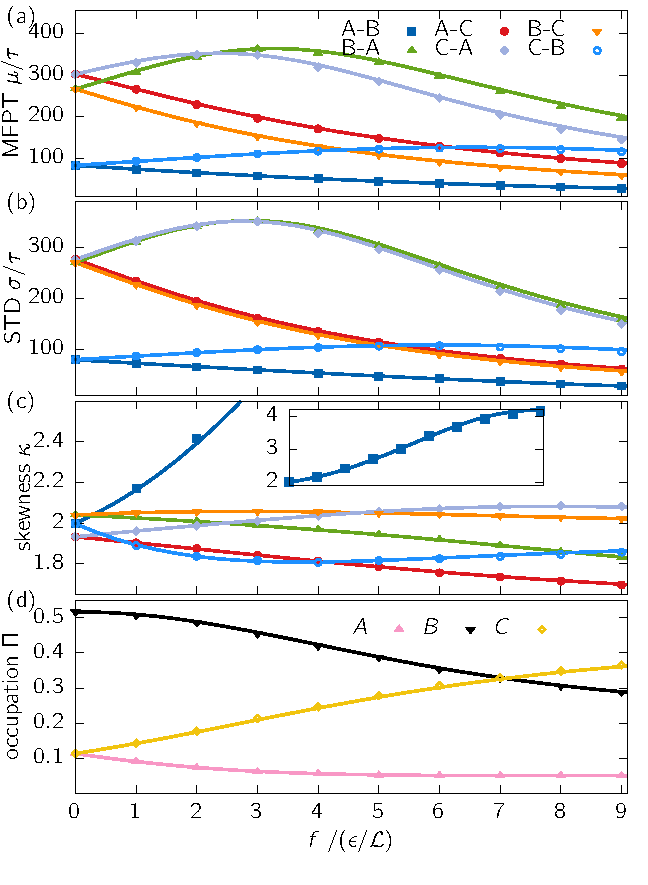
\includegraphics{../plots/Urew/mom_2010.pdf}
 \caption[The first three moments and the population of metastable states for the 1D driven system for varying external force.]{(a-c) The first three moments of the FPTD for all six processes between metastable states in figure~\ref{fig:potgl}a under varying external force $f$. (d) The occupation probability of each metastable state. The dots represent the value measured from simulation. The line is the equilibrium system continuously reweighted.  }
 \label{fig:momgl}
\end{figure}
\FloatBarrier

\section{Single Particle in 1D under Local Driving}
\label{sec:Lasersys}
\begin{figure}[h]
\centering
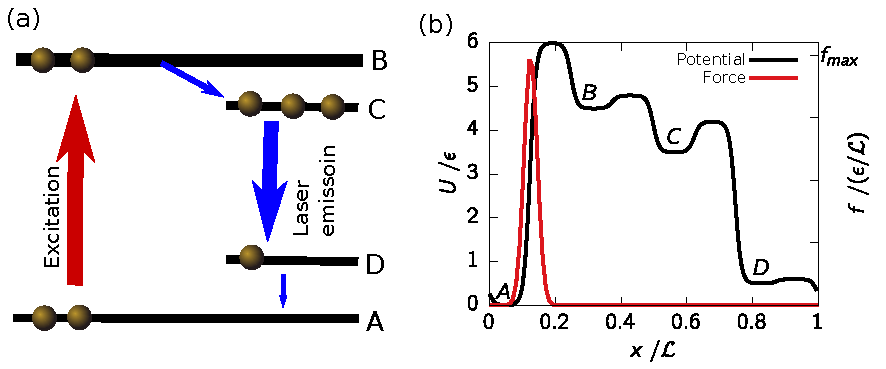
\includegraphics{../images/laser.pdf}
\caption[Sketch of a 4-state laser model with potential surface and pumping force.]{ (a) Sketch of a 4-state laser model. The electron are pumped from state $A$ to state $B$, marked by the red arrow. The blue arrows represent relaxation transition. The transition $C \rightarrow D$ relaxes under emission of a photon. (b) Translation of laser model to a continuous potential surface. The excitation is represented by a Gaussian force in the direction of the potential barrier.  }
\label{fig:laser}
\end{figure}

\begin{figure}[t]
\centering
 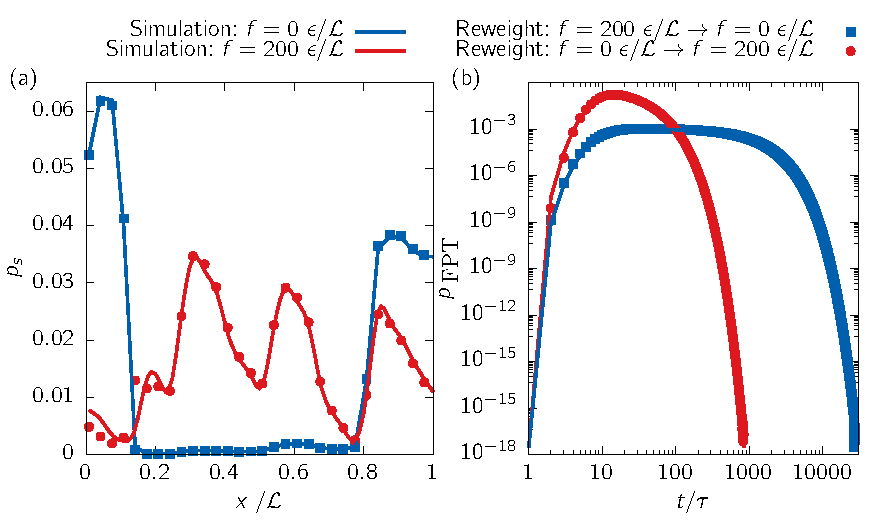
\includegraphics{../plots/Urew/single_9040.pdf}
 \caption[Stationary distribution and first-passage time distribution of the excitation process for the laser model.]{(a) stationary distribution and (b) FPTD of the excitation process $ A \rightarrow B$. The lines in (a,b) represent the results from simulating a single particle in the potential without (blue) and with (red) external force. The dots are the results from reweighting the systems into each other. }
 \label{fig:singleL}
\end{figure}

This model is inspired by a laser model with 4 states. A laser is in a far-off-equilibrium steady state and shows population inversion where high energy electron states are more populated than low energy states~\cite{kaschke2013optical}. Relaxing electrons from the high energy state to a low energy state emits photons. The steady state is driven by an external force pumping  electron to higher energetic states. The laser starts emitting monochromatic light when the higher energy states are more  populated than the lower states. 

An electron in figure~\ref{fig:laser} starting in state $A$ is pushed to the highest energetic state $B$ by external driving. Typically, the energy is provided by optical illumination and photon absorption, chemical reactions or electronic discharge~\cite{kaschke2013optical}. In this simplified model, the driving is represented by a Gaussian shaped force irrespective of the source. From the highest state, it relaxes fast to a state $C$ with slightly lower energy under emission of heat in form of vibrations to surrounding atoms. This state is used to depopulate state $B$, so it can be repopulated quickly by the pumping. The electron relaxes from state $C$ to $D$  by emitting a photon. In practice the emission may happen by spontaneous or stimulated emission. The  relaxation from state $D$ to $A$ is fast under the emission of vibrational energy to surrounding atoms like the transition $B \rightarrow C$. 
The depopulation of state $D$ will promote the desired transition $C \rightarrow D$. Direct transitions between non-neighbouring states like $B \rightarrow D$ are forbidden by the selection rules of quantum mechanics. All described transition may occur the other way round by random fluctuations. The pumping will promote the described path and suppress the inverse path. Without this pumping, the forward and backward transition becomes equally likely, i.e. the system fulfils detailed balance and Boltzmann statistics apply. The flow in cycles is essential for a NESS. That means a 3-state laser model can be constructed by deleting supporting states $B$ or $D$ and it can show population inversion too. A 2-state laser would automatically fulfil detailed balance and cannot show population inversion.

The model is not designed to be an accurate presentation for a laser. The helium-neon-laser for example uses 3 states of the helium and 6 states of the neon gas~\cite{leach2014fundamental}. The number of states, the barriers and energy levels are chosen purely phenomenological. The transition states are modelled by a steep potential slope and the classical Langevin equation does not represent quantum mechanical transitions. There is only a single particle in the system, i.e. the electron is non-interacting. The model is designed to achieve a complete population inversion, where the equilibrium occupation order is inverted for all four states. It shows that the equilibrium and driven states share less dynamics than in the previous 1D system. The reweighting procedure requires reliable reference data, so this model is challenges it by the absence of common dynamics. Furthermore, the reweighting procedure is challenged by external forces that act locally.

The MSM was constructed with $64$ microstates and a lagtime of $0.002\,\mathcal{T}$. The equilibrium system and a system driven at peak force $200\,\frac{\epsilon}{\mathcal{L}}$ is compared in figure~\ref{fig:singleL}. It should be noted that the peak force is 20 times larger than external forces used in previous systems.  The stationary distribution is recreated well by the reweighting procedure. There is a small artifact at the peak of the external force for the reweighted driven system. The FPTD is shown for the pumped transition from $A$ to $B$. The short-time processes are more probable by a factor of 10 for the pumped process compared to the equilibrium process. The equilibrium system shows transition over the whole spectrum from $10$ to $10000$ Markovian steps. The reweighting procedure recovers the FPTD for both systems although transition times differs by a factor of 10. 

The comparison for different driving forces by the first three moments of the FPTD and the metastable state population is shown in figure~\ref{fig:momL}. The analysis shows the pumping and emission transition and their corresponding inverse transition. Note the logarithmic scale in MFPT and STD to capture the large differences in timescales of the observed systems. The MFPT of the pumping transition $A \rightarrow B$ speeds up drastically as desired. The inverse transition opposing the pumping is affected much less and the mean increases slowly. The duration of the desired relaxation transition $C \rightarrow D$ is unaffected by the pumping. However, the transition is happening more frequently because state $C$ is much higher populated than in equilibrium. The inverse relaxation $D \rightarrow C$  speeds up with the pumping  caused by the cyclic motion via $A$ and $B$, not by a direct jump. Again, the STD follows the behaviour of the mean, also in magnitude. The skewness does not show any new behaviour, the skewness of transition $A \rightarrow B$ is increasing when approaching low MFPT. The stationary distribution shows the first population inversion of state $B$ and $C$ for $ f> 70\,\epsilon / \mathcal{L}$. The populations are globally inverted for $f > 170\,\epsilon / \mathcal{L}$.

Simulation and reweighting from equilibrium agree well, but some deviation can be seen for increased driving. Major deviations occur in the MFPT and the skewness of the NESS of transition $A \rightarrow B$ for driving $f >\,150 \epsilon / \mathcal{L}$. The MFPT is underestimated due to the defect in stationary distribution shown in figure~\ref{fig:singleL}a. This deviation can be an effect of the discretisation of state. The localised Gaussian force is continuous in simulation and discretised in the reweighting procedure, where it spreads out over just a few microstates in the MSM. The local error does not effect other transitions.  The reweighting procedure can capture localised forces but the microstates should be chosen fine so the discretised description of the forces is sufficient. Most of the deviations occur when the driving is very large compared to previous driving forces. The large deviation in skewness is connected to the same effect for very low MFPT described for the previous systems. The method relies on sufficient data from the reference simulation. The underlying dynamics of both processes are so different that deviations can occur because the reference sampling is noisy, similar to the effect of missing reference data in equilibrium reweighting (see section~\ref{sec:rewEqu}).  Furthermore, the MSM was constructed for the reference system. The dynamics of the driven system are much faster and the lagtime can be too large to describe the system properly.   Considering these effects, deviations for heavy driving are in an acceptable range. 


We achieved the desired total population inversion as a limitation test for the reweighting procedure. It shows that far-off equilibrium phenomena are captured by the reweighting, despite the approximation close to detailed balance for a single jump. The construction of long trajectories from single transitions marginalises the error.  The effect of local forces was tested in depth. The model demonstrates that local entropy productions are essential for NESS, a global constraints would not be able to capture the local driving in this model. 


\begin{figure}
\centering
 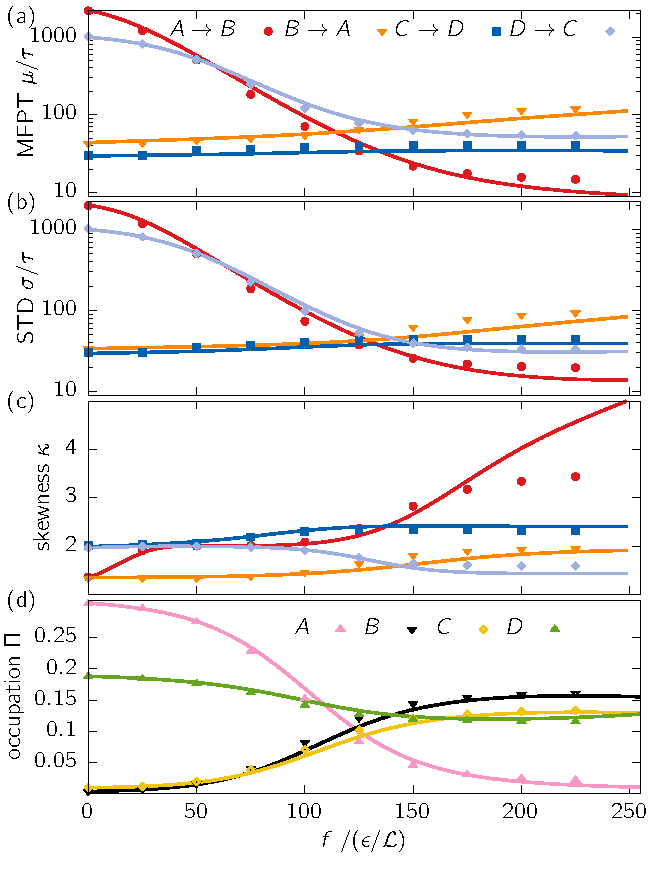
\includegraphics{../plots/Urew/mom_9040.pdf}
 \caption[The first three moments and the population of metastable states for the laser system for varying external force.]{(a-c) The first three moments of chosen FPTD between metastable states in figure~\ref{fig:singleL} under varying external force $f$. The transition are the pumping transition $A \rightarrow B$ and the emission transition $C \rightarrow D$ with both inverse transitions. (d) The occupation probability of each metastable state. Full population inversion for driving $f >\,170 \epsilon / \mathcal{L}$.  The dots represent the value measured from simulation. The line is the equilibrium system continuously reweighted. }
 \label{fig:momL}
\end{figure}
\FloatBarrier

\section{Single Particle in 2D under Global Driving} 
\label{sec:2Dsys}

\begin{figure}
\vspace{-0cm}
\centering
 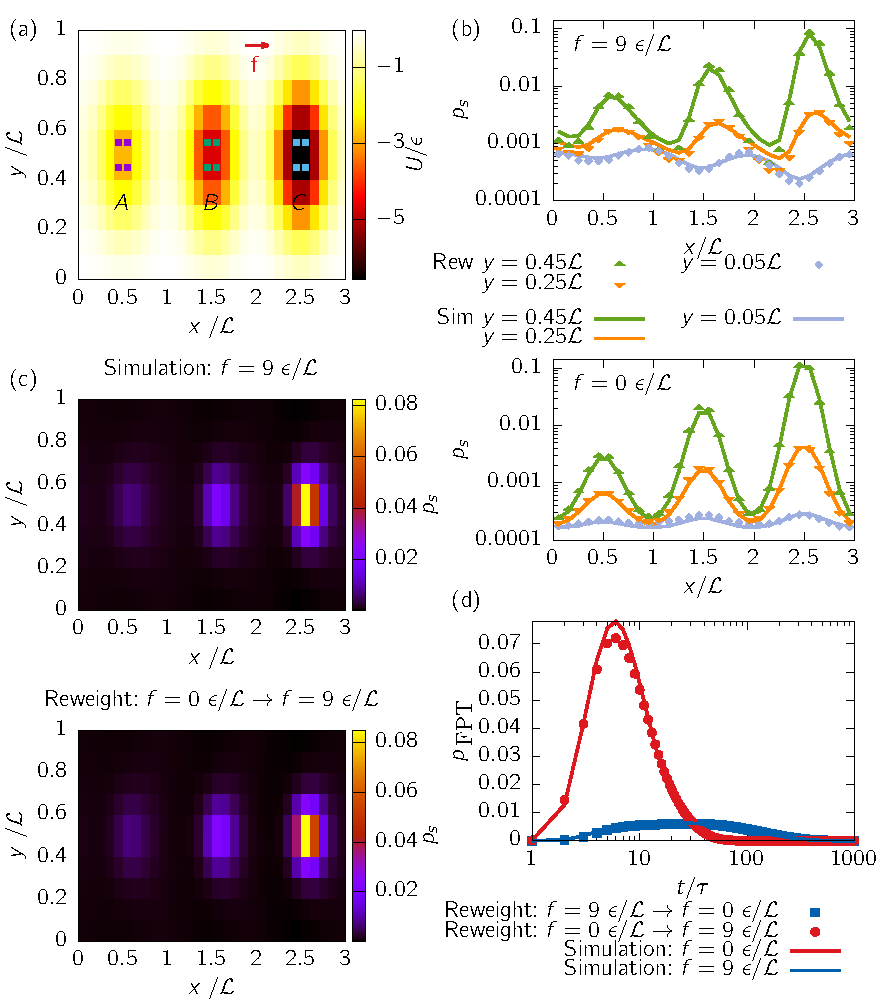
\includegraphics{../plots/Urew/single_5010.pdf}
 \caption[Potential surface, stationary distribution and first-passage time distribution of a chosen process for the 2D driven system]{(a) The potential surface with the metastable states marked $A$, $B$, $C$. (b) Stationary distribution under driving from simulation and from reweighting. (c) Detailed view on the stationary distribution in equilibrium and driven with $9\,\frac{\epsilon}{\mathcal{L}}$ on states with $y=0.05\,\mathcal{L}, 0.25\,\mathcal{L}, 0.45\,\mathcal{L}$. The lines are the results from simulation, the dots from reweigthing into each other. (d) FPTD of the process $ C \rightarrow B$. The lines represent the results from simulating a single particle in the potential without (blue) and with (red) external force. The dots are the results from reweighting the systems into each other.  }
 \label{fig:pot2D}
\end{figure} 

The non-interacting particle is suspended in a 2D potential to introduce a second degree of freedom that has to be recovered correctly. The configuration space increases quadratically and challenges the reweighting method by a large number of microstates. 

The potential consists of three Gaussian potential wells of varying depth, shown in figure~\ref{fig:pot2D}a. All boundaries are periodic and the external force is applied along the $x$-direction. The microstates consists of $30$x$10$ squares of equal size, the lagtime was chosen at $0.02\,\mathcal{T}$. The potential minima were chosen at $3\,\epsilon$, $5\,\epsilon$ ,and $7\,\epsilon$, located on a line in the middle of the y-axis. The STD of the Gaussian is $0.02\,\mathcal{L}$ in both directions.    

A detailed view on the stationary distribution is given in figure~\ref{fig:pot2D}c. The simulated system at $9\,\frac{\epsilon}{\mathcal{L}}$ and the reweighted system agree in probability distribution at first sight. Figure~\ref{fig:pot2D}b adds the probabilities distribution for $(i)$ a $y$-value along the middle of the system, $(ii)$ one at boundary of the system and $(iii)$ one in the middle of these two, comparing the simulated and reweighted stationary distribution.  The probability density around the minima decreases with driving and more states surrounding the minima are occupied. Within the basins, the distribution is tilted in the direction of the force. Turning to the result of reweighting, the logarithmic scale reveals a deviation when reweighting from equilibrium to the driven system. The error is smaller reweighting vice versa. The occupation probabilities between the basins are estimated too low and in the minima too high. This error was not identified for the 1D-systems and it is more pronounced in the driven than in the equilibrium system. Turning to figure~\ref{fig:pot2D}d the FPTD of the transition $C \rightarrow B$ peaks at faster processes for the driven system because the transition via $A$ becomes more prominent. The equilibrium transitions occur at a broader probability peaking between $10\,\tau-30\,\tau$.  A small deviation between simulation and reweighting can be seen at the peak of the driven distribution. The process speeds up by a factor of $10$.    
\begin{figure}
\centering
 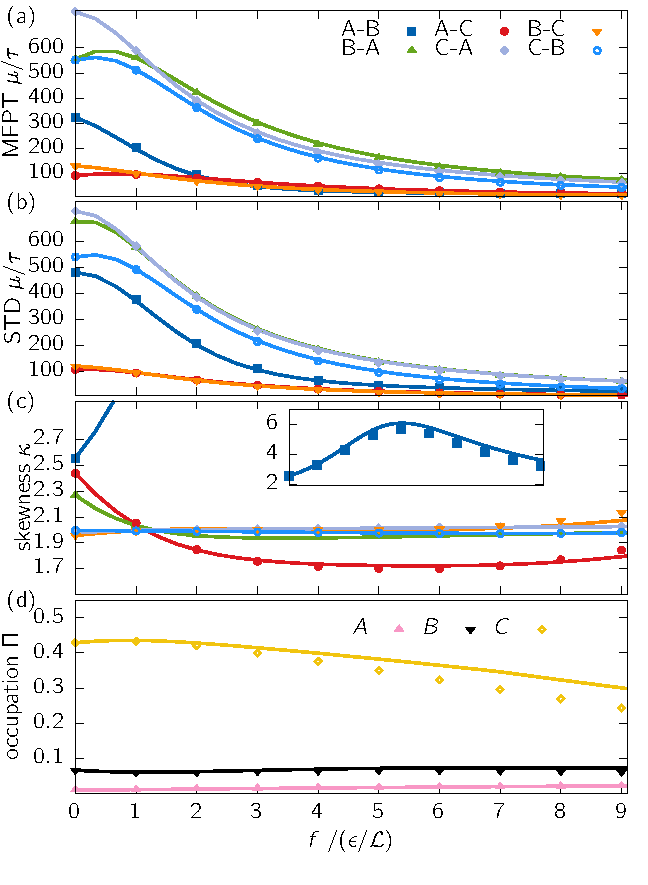
\includegraphics{../plots/Urew/mom_5010.pdf}
 \caption[The first three moments and the population of metastable states for the 2D system for varying external force.]{ (a-c) The first three moments of the FPTD for all six processes between metastable states in figure~\ref{fig:pot2D}a under varying external force $f$. (d) The occupation probability of each metastable state. The dots represent the value measured from simulation. The line is the equilibrium system continuously reweighted. }
 \label{fig:mom2D}
\end{figure}

The first three moments of the six slowest FPTD and the metastable state occupation probability is shown in figure~\ref{fig:mom2D}. The MFPT becomes faster for all processes under driving. Only the processes $C \rightarrow B$ and $B \rightarrow A$ slow down for small driving before speeding up. Similar to the 1D system in section~\ref{sec:1gl}, this can be explained by an initial slowing down by the particles taking the direct path against the force. For larger driving the spatially longer paths along the external force become more prominent and increase speed of the process. Compared to the 1D system under global driving, this phenomena comes into effect for much lower driving although the potential barriers are larger.  A possible reason is the bypassing of the intermediate state because the potential barriers are small close to the $y$-boundaries. The increase in occupation probability in $y$-direction supports this argument, because more trajectories pass by these states. Again, the STD shows the same trend as the MFPT. The skewness levels $\approx 2$ again. The process $A \rightarrow B$ shows abnormal behaviour in skewness by increasing until $4\,\frac{\epsilon}{\mathcal{L}}$ and then decreasing again. The skewness of process $A \rightarrow C$ on the other hand becomes smaller than than for the other processes, indicating a tilting of the distribution to the right. Both effects can be explained with another set of slower processes entering the system for increasing driving: The potential in $A$ is a too weak obstacle for the particle flowing by.
\begin{figure}[t]
\centering
 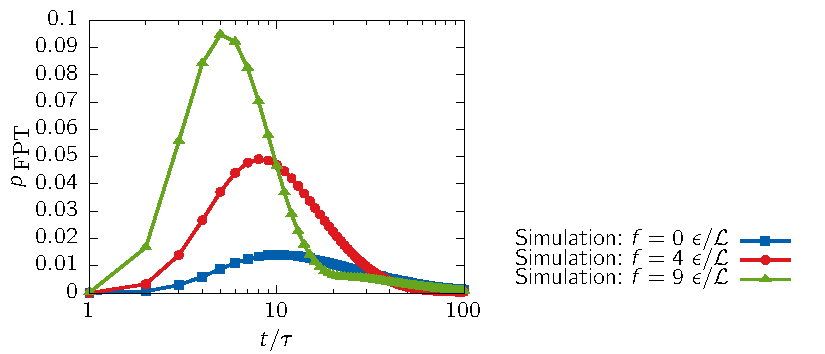
\includegraphics{../plots/Urew/fpt_5010.pdf}
 \caption[First-passage time distribution of transition $A \rightarrow B$ simulated at 3 different driving forces for the 2 system.]{FPTD of transition $A \rightarrow B$ simulated at 3 different driving forces. Increased driving promotes short-time processes and suppresses slow processes. For $f =9\,\frac{\epsilon}{\mathcal{L}}$ a second peak appears at $\approx 30\,\tau$, showing new long-term processes.  }
 \label{fig:fpt2D}
\end{figure}
There is an increasing probability that they simply bypass the metastable state lying in the minimum of the potential and produce trajectories longer than the system size. The effect is shown in figure~\ref{fig:fpt2D} where increased driving results in an increase of short-time processes in $A \rightarrow B$ on the left-hand-side of the distribution. Further driving produces a second small peak on the right-hand-side, showing the long-time processes bypassing $A$. The decrease in MFPT is slowing down and the skewness  decreases by this effect. The bypassing can only occur for a 2D system.  The metastable state occupation in figure~\ref{fig:mom2D} of state $C$ decreases and occupation of state $A$ and $B$ stay approximately the same. The depopulation of the highest probability state was seen in the 1D system too. The other states do not increase in population because the probability generally spreads out from the potentials minima. A broader definition of metastable states would capture this in an increase of occupation probability with increasing driving. The reweighting procedure has problems capturing the true magnitude of $C$ as discussed earlier in the detailed view on the stationary distribution in figure~\ref{fig:pot2D}. 

The reweighting technique shows excellent results for this model too. We can see some deviation, e.g. for the peak of the FPTD in figure~\ref{fig:pot2D}d or the occupation probability between the basins in figure~\ref{fig:pot2D}b. Both effects only take place when reweighting over a broad range of driving. The additional degree of freedom requires a larger number of microstates and defines a challenge for the reweighting procedure and gives insight in its possible limitations. In particular we find that states away from the basins are not recovered correctly by the reweighting. The sources of deviation for all systems will be discussed in detail in the next chapter. 



\FloatBarrier
\section{Discussion}
The previous sections applied the reweighting scheme to a number of different systems, all being single particles in different external potentials under varying driving forces. The potential surface and the external forces can be varied locally once an MSM for a reference system is created. The gathered information can be reweighted to any other system, as long as it is similar to the reference system. This section discusses the precision and limitation of this method.

The method needs two sets of input data: Any reference data in form of an MSM and the local entropy production of the target system. The latter can be included by the total entropy production $\Delta S_{ij}$ from state $i$ to $j$ or by the difference in entropy production of reference and target system $\Delta S_{ij} - \Delta S^q_{ij}$ as shown in equation~\ref{eq:finalpij}. Any system can be chosen for a reference, indicating that there is an underlying invariance in the reference systems, as it was introduced in equation~\ref{sec:Invariant}. This consequences of the invariant is further discussed in section~\ref{sec:InvariantC}. 

The method relies on sampling transition probabilities of a system sufficiently. The underlying simulated trajectories give a more detailed picture but are broken into pieces of local transitions. Sampling the transition probabilities is a much easier task than sampling complete trajectories. As a result trajectories that do not exist in the reference system are constructed by the MSM of the reweighted system. This can be seen in the FPTD for all systems (see figure~\ref{fig:potequ}, \ref{fig:potgl} , \ref{fig:singleL}, \ref{fig:pot2D}). The underlying MSM allows us to construct trajectories that are important in the target system. This is a fundamental difference to the Ferrenberg-Swendsen reweighting for equilibrium introduced in section~\ref{sec:rewEqu}: The method fails if states required in the target system are not sufficiently sampled in the reference system. Translated to dynamics, it means that the important transition probabilities of the target system have to be sampled sufficiently in the reference system. The complete trajectories do not need to overlap because they can be constructed afterwards. The locality of the entropy productions is key for the system to work because each part of the trajectory is reweighted individually to constitute the local nature of non-equilibrium processes. The global balance condition account for the interaction of all microtransition.

The MFPT and the STD of the FPTDs show similar trend and magnitude for all systems. Exponential distribution have the property $\sigma = \mu$. The large tails of the FPTDs decay exponentially and dominate the variance of the system. The observed values for mean and STD become  similar for our systems but not equal because they deviate from exponential distributions for short time processes.  

\subsection{Sources of Error}
\label{sec:Error}
The FPTD shows small deviations from its expected distribution with increasing reweighting distance. This deviation is largest in the peaks of the FPTD distribution and for the stationary distribution of the 2D system in figure~\ref{fig:mom2D}. Error analysis was performed on different systems to exclude sampling issues. Other sources of the deviation are possible and are discussed in the following:

\begin{itemize}
 \item The approximation was used in the deviation of the reweighting formula
 \item Insufficient constraints in the Maximum Caliber
 \item Chosen microstates and lagtime of reference MSM might be unsuitable for target system
 \item Limitation for large fluctuations
\end{itemize}

The necessity of the approximation was discussed in detail in section~\ref{sec:numerics}. The exact set of equations emerging from the Caliber cannot be solved numerically. Furthermore the full set of equation may have more than one solution and it cannot be guaranteed to find the correct one. The approximation solves this issue by having a singular solution and fulfilling the constraints of the Caliber. The significance of this error cannot be determined without an available full solution. 
 
Constraining the Caliber according to the local entropy production is based on how the system interacts with its environment. Global balance is introduced to model the internal connection of the states. Success of the method is based on the quality of the constraints. It cannot be excluded that other effects play a major role. If other effects exist they are minor for the given systems. If new constraints can be identified it can be included in the Caliber in form of Lagrangian multipliers. For now we assume the set of constraint to be complete.

Another source of error is based on the construction of the Markov State Model. The microstates are chosen equi-sized and independent of data so all models can be represented by it. The lagtime on the other hand is chosen based on a method  requiring equilibrium data (see section~\ref{sec:MSM}). The method fails for NESS, so the lagtime of the reference equilibrium system is assumed to be valid for the target system too. When reweighting over large distances this assumption might be flawed. An indicator is the MFPT that changes considerably e.g. for the laser system. This suggests a change in timescale and the lagtime of the target MSM might be chosen inconsistent with the Markovian assumption. The user has to reweight MSMs constructed at different lagtimes to check for deviations based on this issue. 

\begin{Technical Point}[tp]

\begin{minipage}{0.03\textwidth}
\hfill\vspace{0.1cm}
\end{minipage}%
\begin{minipage}{0.35\textwidth}
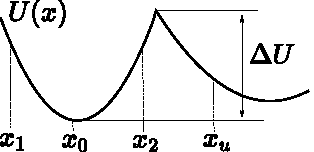
\includegraphics{../images/kramers.pdf}
\end{minipage}
\hfill
\begin{minipage}{0.6\textwidth}
The Kramers model~\cite{kramers1940brownian} describes non-dissipative dynamics of molecular reactions by a 1-dimensional potential $U(x)$ coupled to a head-bath at temperature $T$ with coupling constant $\gamma$. It estimates the rate of a transitioning over a barrier by 
\end{minipage}
\begin{equation*} 
 k = \frac{k_{\mathrm{B} }T}{\gamma} \left ( \int_{x_0}^{x_u} \exp \left ( \frac{U(x)}{k_{\mathrm{B} }T} \right ) \int_{x_1}^{x_2} \exp \left ( \frac{-U(x)}{k_{\mathrm{B} }T} \right )\right )^{-1}
\end{equation*}
The first integral is over the transition region, the second integral captures the starting potential or the initial probability distribution. Kramers showed 
how the transition rate depends on the form and the height of the potential. It requires that the equilibration time $\tau_e$ in one basin is much smaller than the transition times $\tau_t \gg \tau_e$. To be consistent we have to assume that $k_{\mathrm{B} }T \ll \Delta U$.
% 

\caption{The Kramers Model}\label{tec:kramers}
\end{Technical Point} 


The method is limited to systems where fluctuations are not stronger than the potential surface. Tests showed that potential barriers of $ \Delta U < k_{\mathrm{B} }T$ are not captured well by the reweighting method. The random fluctuation takes over the system-dependent local entropy productions.  The barrier crossing dynamics are governed by the local potentials and captured well (see technical point~\ref{tec:kramers}). The diffusion dynamics governed by symmetric fluctuations on the other hand are not well captured. This effect can be seen in the 2D system in figure~\ref{fig:mom2D} where trajectories bypass some potential minima for heavy driving. The potential barrier close to the boundary in $y$-direction is often smaller than kinetic energy from fluctuations. Once these states show larger population, the error becomes more pronounced. The presented errors for heavy driving might emerge from this limitation of the method. 

The mentioned sources of errors are oftentimes difficult to check. However, this chapter shows that the errors are minimal compared to the range of the reweighting method. Even increasing/decreasing the speed of processes by the order of 10 is captured with minor deviation. A full error analysis on the construction of the MSM or developing a maximisation algorithm for the full solution of the Caliber can be useful for future investigation.  The presented data proves the concept of Caliber maximisation under constraining global balance and local entropy production by reweighting MSM between NESS. The proposed combination of constraints form a functional ensemble for NESS at different temperatures, different potentials and various strength and form of driving.    


% % 
% \bibliography{/home/marius/PhD/Thesis/references.bib}
% \bibliographystyle{plain}
% \end{document}

% 
% \documentclass[paper=a4,fontsize=12pt,open=right,noabbrev]{report}
% \documentclass[12pt]{report}
% \usepackage[utf8]{inputenc}
% \usepackage{amsmath}
% \usepackage{amssymb}
% \usepackage{graphicx}
% \usepackage{placeins}
% \usepackage{cite}
% \usepackage{physics}
% \usepackage{mathrsfs}
% \usepackage{geometry}
% 
%  \setlength{\parindent}{0em}
% \setlength{\parskip}{1em}
%  
% 
% \begin{document}

 
\chapter{Reweighting Dynamics by Collective Variables} 
Complex systems consist of many particles giving rise to pair and higher order  interactions. The large number of interactions is burdensome to analyse and display for interpretation. One typically reduces the high-dimensional space to a few low-dimensional variables describing the slowest dynamical processes of the system. This reduction implies that the remaining coordinates average out on faster timescales or have no effect on the process of interest. The system is reduced to the chosen aspects and is not under full investigation. Examples are the description of a magnet by its magnetisation whilst ignoring the influence of local dipole fluctuations~\cite{tobik2017free} or the crystallisation of particles described by the closest radial environment of each crystallising particle~\cite{radhakrishnan2003nucleation}.  Fast and local processes are  integrated out when deciding on a set of collective variables. This is compatible with Markov State Model (MSM)  construction because here, fast processes are neglected too. However, the mesoscopic descriptors or \textit{collective variables}(CV) are chosen system-specific and the choice limits the view on the system: The crystallisation described by the local environment of the particles holds detailed view on the crystalline phase but limited information on the liquid phase~\cite{radhakrishnan2003nucleation}. Furthermore, a poor choice of CVs can hide important processes and free energy barriers or cause an inaccurate estimation of implied timescales~\cite{bolhuis2000reaction,valsson2016enhancing,noe2017collective}. Dimensionality reduction and choice of an advantageous set of collective variables is a widely discussed research field on its own and is applied to describe complex systems in chemistry, biology, physics and more~\cite{rohrdanz2013discovering}. 

MSM requires the use of CVs to be computationally accessible. State of the art use $10^2 - 10^3$ microstates~\cite{noe2019markov}, resulting in $10^4 - 10^6$ possible transitions that have to be sampled. A construction on the full conformational space requires a larger number of transitions that would  exceed computational boundaries and we use collective variables to bypass these limitation. This chapter tests the reweighting procedure on systems described by collective variables to extend its scope to a larger group of systems.
The reweighting method is first applied to a particle in a 2D-potential described by a 1-dimensional collective variable. The second test system is a coarse-grained tetraalanine peptide being described by CV and showing many-body interactions.

The reweighting procedure can be applied without adjustment. The collective variables hide the full local entropy productions, but the relative local entropy productions
\begin{equation}
 \Delta S_{ij} - \Delta S_{ij}^q = \frac{ \Delta U(x_j) - \Delta U(x_i) + (x_j - x_i) \Delta f }{k_{\mathrm{B}} T}
 \end{equation}
 is sufficient for reweighting. Here, $\Delta U(x)$ is the change in potential and $\Delta f$ is the change in force of reference and target system. The new potentials or forces are defined for the CVs coordinate $x$, unlike in the previous chapter for the conformational coordinates.  We only need to know the change in local entropy productions $\Delta S_{ij} - \Delta S_{ij}^q$ due to driving from theoretical prediction. Since the forces and potentials are aligned with the CVs we can calculate them. The total local entropy productions $\Delta S_{ij}$ are not known from theory anymore. The total values are sampled by the reference simulation itself. 

\section{Single Particle in Collective Variable Space} 
As a first testing ground we choose the 2D system from section~\ref{sec:2Dsys} and integrate out the $y-$dimension orthogonal to the driving force, shown in figure~\ref{fig:potred}a,b. This will imitate the reduction to a collective variable on the testing ground of the well-understood minimal system. A MSM is constructed on the reduced space.

\begin{figure}
 \centering
 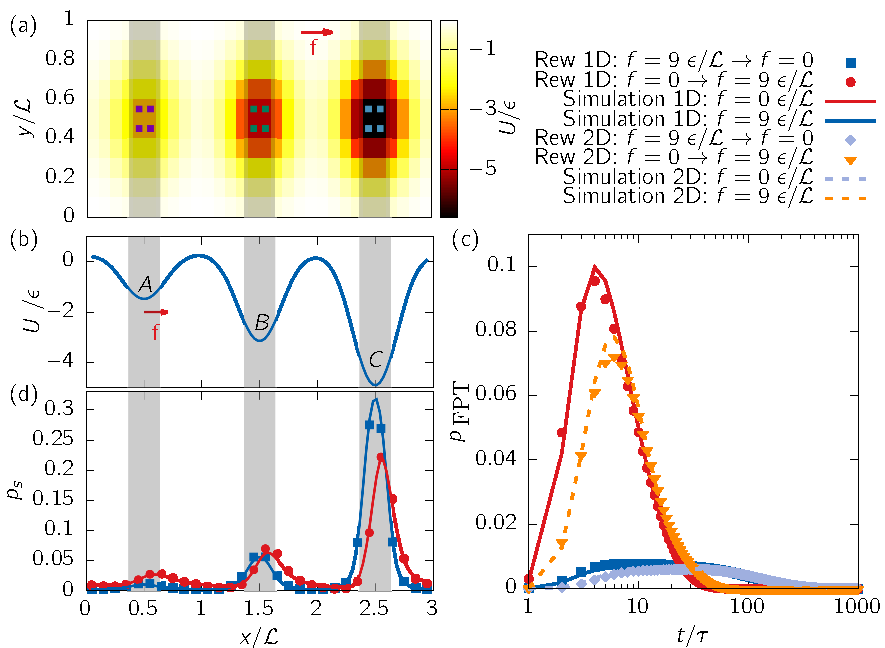
\includegraphics{../plots/Frew/single_1030.pdf}
 \caption[Free energy surface, stationary distribution and first-passage time distribution of a chosen process for the 1D reduced system]{ (a) The 2D potential with the three metastable states indicated by squares. Integrating out the $y-$dimension gives (b) the mean potential of the equilibrium system. The grey area represents the new metastable states $A$,$B$,$C$. The area of the metastable state is effectively increased.  (d) The stationary distribution of the reduced system and (c) FPTD of the process  $C\rightarrow B$. The lines in (c,d) represent the results from simulating a single particle without (blue) and with (red) external force. The dots are the results from reweighting the systems into each other. The orange and light-blue dashed lines show the same process for the underlying 2D process with dots representing the reweighted FPTD.  }
 \label{fig:potred}
\end{figure} 
 
The 2-dimensional system is reduced by integrating along the $y-$axis of the system. A mean force and mean potential is calculated by
\begin{equation}
\begin{aligned}
  \langle \mathbf{F} (x) \rangle &= \int \dd{y} \mathbf{F}_{\text{2D}}(x,y) \pi(x,y) \\
  \langle U (x) \rangle &= \int \dd{y} U_{\text{2D}}(x,y) \pi(x,y) .
\end{aligned}
\end{equation}
Note that the definition of the mean potential is only valid for the equilibrium system and a potential cannot be defined off-equilibrium. The position of the metastable states are determined from the $x$-coordinate of the 2D system to compare the dynamics of full and reduced system. The dimensional reduced data are collected during runtime of the full systems simulation. A MSM is constructed with the same lagtime $\tau=0.02\,\mathcal{T}$ and the same 30 equi-sized microstates in $x$-direction. 

Figure~\ref{fig:potred}c and d compares the first-passage time distribution (FPTD) and the stationary distribution of the reduced system in equilibrium and under driving of $9\,\frac{\epsilon}{\mathcal{L}}$ when reweighting the systems into each other.  The FPTD of the 2D system in full conformational space is shown for comparison. Small deviations are seen in the FPTD, however, they are of the same magnitude and position as the reference 2D system. The reweighting for short processes of $1-5\,\tau$ are overestimated, whereas the peak is underestimated in both cases. The tail for longer processes is reweighted correctly. According to the results shown in figure~\ref{fig:potred}d, the stationary distribution is recreated by the reweighting procedure.  We deduce that the reweighting works well, even though system's details are lost by the used collective variables. An impairing effect on the reweighting cannot be observed for this system.  The mentioned deviations are based on deviations on the reweighting in the underlying 2D-system in full conformational space.
\begin{figure}
\centering
 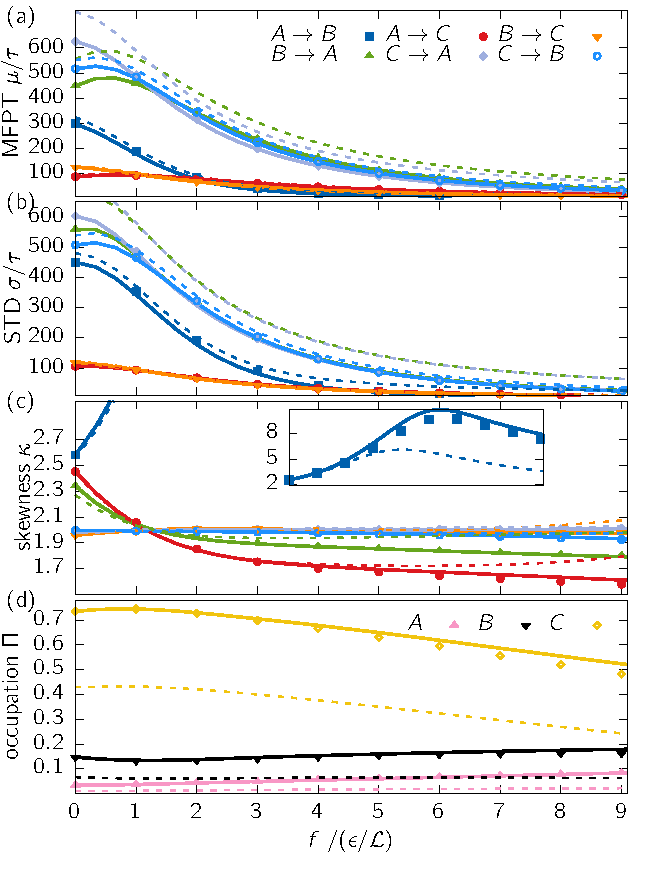
\includegraphics{../plots/Frew/mom_1030.pdf}
 \caption[The first three moments and the population of metastable states for the reduced 1D system for varying driving forces.]{(a-c) The first three moments of the FPTD for all six processes between metastable states defined in figure~\ref{fig:potred}b under varying external force $f$. (d) The occupation probability of each metastable state. The dots represent the value measured from simulation. The line is the equilibrium system continuously reweighted. The dashed lines are the processes of the underlying processes in 2D space.  }
 \label{fig:momred}
\end{figure}

Figure~\ref{fig:momred} shows continuous reweighting from the equilibrium system for the first three moments of the FPTD between metastable states and the occupation probability $\Pi$ of each metastable state. Additionally, the reweighting from the underlying 2D system is shown by dashed lines. First, we focus on comparing results of the 2D system and its reduced system. The mean first-passage time (MFPT) is responding to external driving the same in both systems. The processes along the driving force speeds up immediately. The processes opposing the driving slow down at first, before the spatially longer path along the external force becomes more probable and the process speeds up too. For all processes the 2D process is slower than the coarse-grained process. This effect of accelerated dynamics is known from coarse-graining different materials~\cite{rudzinski2019recent,depa2005speed,guenza2015thermodynamic,meinel2020loss}. It originates in the disappearance of roughness in the free energy surfaces, resulting in a decrease of effective friction and increase of effective mobility. For our simplified model, this effect reduces the effective potential barriers, leading to the acceleration of the coarse-grained process. The response of full and reduced processes under driving remains qualitatively the same although mobility was not preserved.  

The standard deviation (STD) of the FPTD of the reduced system is lower compared to the 2D system. This agrees with the observation that MFPT and STD behave similarly. The skewness of both systems agree. A deviation of the full and reduced system is seen in the inset of the skewness for  process $A \rightarrow B$. The initial increase in skewness was seen for different systems in chapter~\ref{ch:RewU} based on low discretisation of the FPTD for fast processes. The following drop of skewness was unique for the 2D system and is explained by emergence of another peak of slow processes in the FPTD. This class of processes was identified with trajectories bypassing the metastable state due to heavy driving. This effect of bypassing a metastable state cannot occur in the 1-dimensional description.
\begin{figure}[t]
\centering
 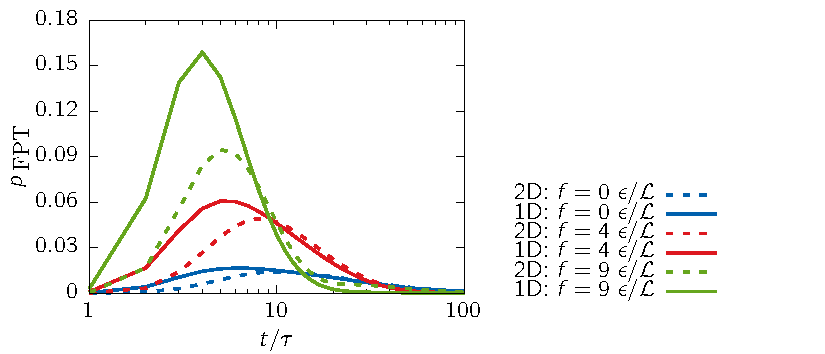
\includegraphics{../plots/Frew/fpt_1030.pdf}
  \caption[First-passage time distribution of transition $A \rightarrow B$ simulated at three different driving forces for the 2D and the reduced model. ]{First-passage time distribution of transition $A \rightarrow B$ simulated at three different driving forces. Increased driving promotes short-time processes and suppresses slow processes. The continuous lines show the FPTD for the reduced system, the dashed lines for the underlying 2D system.   }
 \label{fig:fpt1Dred}
\end{figure}
Figure~\ref{fig:fpt1Dred} shows that the FPTD of the reduced system under driving does not show a second peak. The decrease around $6\,\frac{\epsilon}{\mathcal{L}}$ of the skewness is based on a symmetrising effect on the FPTD of stronger driving. The deviation in skewness of the 2D system and the reduced system is thus based on loss of information of dynamics in $y$-direction  when describing the dynamics by collective variables.  

The occupation probability of the metastable states is considerably larger for the reduced system. The metastable states in the 2D system are smaller because they do not span the whole $y$-direction. The reduction to the $x$-axis enlarges the metastable states effectively and the occupation probability increases. The trend of decreasing occupation in $C$ and increasing occupation $A$ and $B$ is the same for both systems.

In the following, we will discuss to the deviation between simulation of the reduced system and its reweighted properties.  The largest deviation can be seen for the process $A \rightarrow B$, although it is comparable to the deviation of the 2D system for this process shown in figure~\ref{fig:mom2D}. The same observation is made for the deviation in occupation probability of state $C$. The error of the reweighting are much smaller for the other processes. In general the deviations are all of the same shape and relative quantity as for the underlying 2D process. We conclude that the use of collective variables of the system did not affect the reweighting process. Hence, it can be applied to the same extend as the reweighting on configurational space. Deviations of the reweighting are adopted from the underlying errors in configurational reweighting and were discussed in section~\ref{sec:Error}.

From the Maximum Caliber point of view the choice of coordinates does not make a difference. It chooses the system with the most uncertainty, given the prior information and the constraints given --- irrespective of the coordinates. The critical assumptions is made by the CVs: We assume other processes to average out on faster timescales along the process. Here, it means that the fluctuations in $y$-direction average out along the ensemble of trajectories between two basins. It is a reasonable simplification for the present 2D-system, but can be hard to justify for complex systems with other processes involved and more complex CVs. A good choice of CVs is a problem of current research by itself~\cite{rohrdanz2013discovering}. Here, we also have to make sure that the CVs are reasonable for both, the reference and the target system. 




\FloatBarrier

\section{Tetraalanine}
\begin{figure}
\centering
 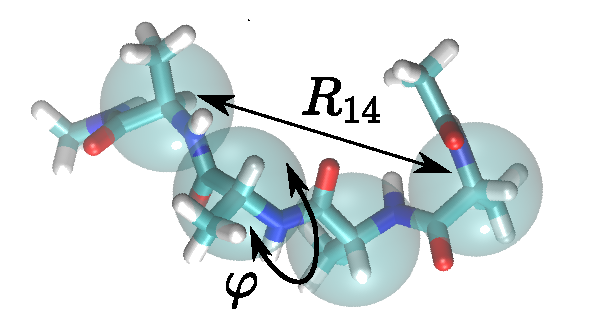
\includegraphics{../images/ala4.pdf}

\caption[Atomistic and coarse-grained representation of the tetraalanine peptide.]{Atomistic and coarse-grained representation of tetraalanine. Atoms are shown as rods,  where turquoise, white, blue, and red represent C, H, N, and O, respectively. The transparent beads show the coarse-grained representation of the system. The end-to-end distance $R_{14}$ and the dihedral angle $\varphi$ are defined for the coarse-grained system. \\
\tiny{Reprinted figure with permission from Tristan Bereau and Joseph F. Rudzinski ,  
Accurate Structure-Based Coarse Graining Leads to Consistent Barrier-Crossing Dynamics, 121(25):256002, 2018 Copyright 2018  by  the American Physical Society. DOI: https://doi.org/10.1103/PhysRevLett.121.256002}}

\label{fig:Ala4}
\end{figure}


\begin{figure}
 \centering
 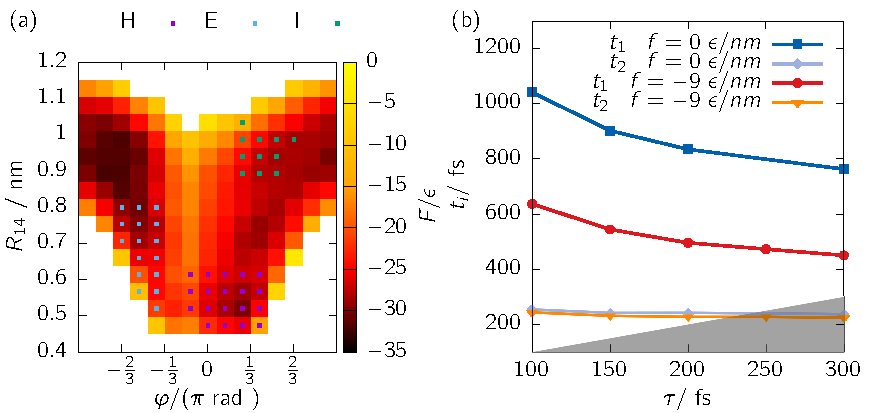
\includegraphics{../plots/Frew/lag_1001.pdf}
 \caption[Free energy surface and lagtime analysis for the two slowest processes of the reference tetraalanine peptide.]{ a) Free energy surface of tetraalanine of the reference system. The metastable states are indicated by H,E,I. (b) Lagtime analysis of the system defined by the reference force field ($f_R=0$) and driven along the end-to-end distance with $f_R = 9\,\frac{\epsilon}{nm}$. The shaded area marks the non-physical area where $t_i < \tau$. }
 \label{fig:AlaLag}
\end{figure}
The following system represents a coarse-grained tetraalanine peptide consisting of four beads.  This model is the first non-artificial material and challenges the reweighting procedure by many-body interactions. External global forces are applied along the CVs to alter the dynamics. These forces may represent an optical tweezer controlling atom distances. The CVs and the forces applied to the system are chosen by the user. The current forces are chosen to test the  effectiveness of the reweighting procedure for conservative and non-conservative forces.

Tetraalanine is a peptide consisting of 44 amino acids and 52 atoms. Each amino acid is coarse-grained to one bead centered at the backbone of the peptide. The coarse-grained force field constructed by Rudzinski and Noid~\cite{rudzinski2015bottom} for the molecule solvated in water consists of 3 pair potentials along the backbone, 2 bending interactions between 3 subsequent beards,  a dihedral angle $\varphi$ between all 4 beads and interaction between the first and the last bead $R_{14}$. The bending interactions are defined by the angle formed between the lines of the first two and last two beads. The dihedral angle is defined by the angle between the planes formed by the first three and last three beads. The MSM is constructed using the end-to-end distance $R_{14}$ and the dihedral angle $\varphi$ as CVs (see figure~\ref{fig:Ala4}), following the example of Bereau and Rudzinski~\cite{bereau2018accurate}. The system will be driven with constant force along both CVs in both directions. The unperturbed system is called the reference system. 
 
The free energy surface of the reference system is shown in figure~\ref{fig:AlaLag}a. Three basins were identified using PCCA+ as introduced in section~\ref{sec:PCCA}. They represent the helical states H, extended state E and one intermediate state I. Note that the direction of driving makes a difference, because the free energy surface lacks the symmetry of the previous systems. The driving along $R_{14}$ can be translated to an additional interaction potential. Systems driven by a force along are still in equilibrium and can be analysed via the eigenvalue decomposition of the transition matrix. Driving along the periodic dihedral angle $\varphi$ will push the system in a non-equilibrium steady state (NESS) that can be analysed using FPTD. 

The lagtime analysis is performed in figure~\ref{fig:AlaLag}b for the reference system and one system driven along $R_{14}$. We choose a lagtime of $200\,$fs to capture the two slowest processes of both systems. The second process is captured by the MSM and is unaffected by the additional forces applied. We expect it to be remain unaffected by larger forces and such it will stay in timescales captured by the MSM. The MSM was constructed with 15 microstates over the range $[-\pi,+\pi]$ in $\varphi$-direction and 15 microstates in the range $[0.45\,\text{nm},1.15\,\text{nm}]$ in $R_{14}$-direction. Two additional sets of microstates were added to collect end-to-end distances outside this range. Energies are given in $\epsilon = \frac{kJ}{mol}$ and the system was simulated at temperature $T = 2.479\,\frac{\epsilon}{k_B}$.

\FloatBarrier
\subsection{Modifying End-to-end Potential}
\label{sec:DrivingEAla}
\begin{figure}
\vspace*{-0.7cm}
\centering
 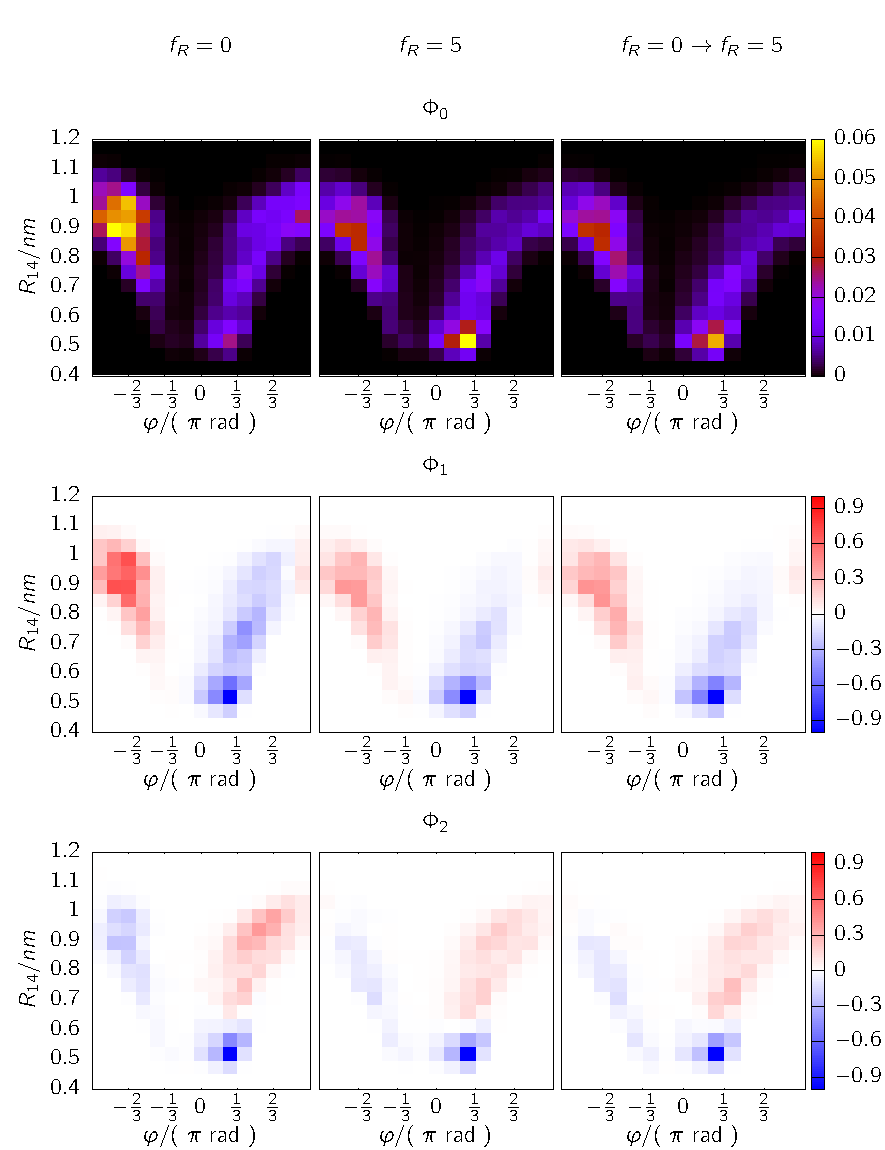
\includegraphics{../plots/Frew/Evec_1002_1902.pdf}
 \caption[Detailed relaxation process analysis of the two slowest processes of the tetraalanine peptide reference model and modified by an end-to-end potential.]{The first row shows the  stationary distribution, the second row the first eigenvector and the third row the second eigenvector of three systems. The system in the first column is the non-perturbed reference system, in the second column the perturbed system at $f=-9\,\frac{\epsilon}{nm}$ and in the third row the reweighted system from reference. }
 \label{fig:EvecAla}
\end{figure}

An optical tweezer uses optical traps to confine beads of a single molecule in harmonic potentials~\cite{jiao2017single}.  We may predict the outcome of such an experiment by applying harmonic potentials of varying strength between the first and the last bead and calculate the effects on statics and dynamics on tetraalanine by reweighting from the undisturbed system. The forces applied are conservative, hence we show an example of reweighting along CVs between equilibrium systems.

At first we have a detailed look at the eigenvectors in figure~\ref{fig:EvecAla} for the system at reference and for driving along $R_{14}$ in negative direction with $f=-9\,\frac{\epsilon}{nm}$. The unperturbed system's stationary distribution shows highest probability at a state with $ \approx 0.9\,$nm end-to-end distance and dihedral angle $\varphi \approx -0.8\,\pi$. This is associated with an extended state. The second minimum can be seen for $\varphi \approx\,0.3 \pi$ and $R_{14} \approx 0.5\,nm$, which is associated with a helical state. A third smaller basin is found at an intermediate state $ \approx 0.9\,$nm and an dihedral angle of $ 0.6\,\pi$. The slowest process describes the transition between the highly populated extended state and the helical and less populated intermediate state over the large barriers around $0\,\pi$ or $1\,\pi$. This second slowest process describes a transition for $\pi>0$ on the right-hand side of the large barrier in the middle, between the helical state and the intermediate state. 


Focusing on the effect of the driving, here, the driving forces the ends together and effectively pushes the stationary distribution to the folded state.  Therefore, the basin of the helical states is more populated than without driving. As shown by the first eigenvector, the slowest process changes and the polymer folds directly in the helical state.  The intermediate state at $0.6\,\pi$ is less important for this process when the additional force is applied. The timescale indicates that the folding occurs faster. The second slowest process is the transition on the right-hand side of the centered barrier and remains unaffected by the driving. We note that 
reweighting to the driven system from the reference system recovers this detailed view on the slowest process correctly.


\begin{figure}
\centering
 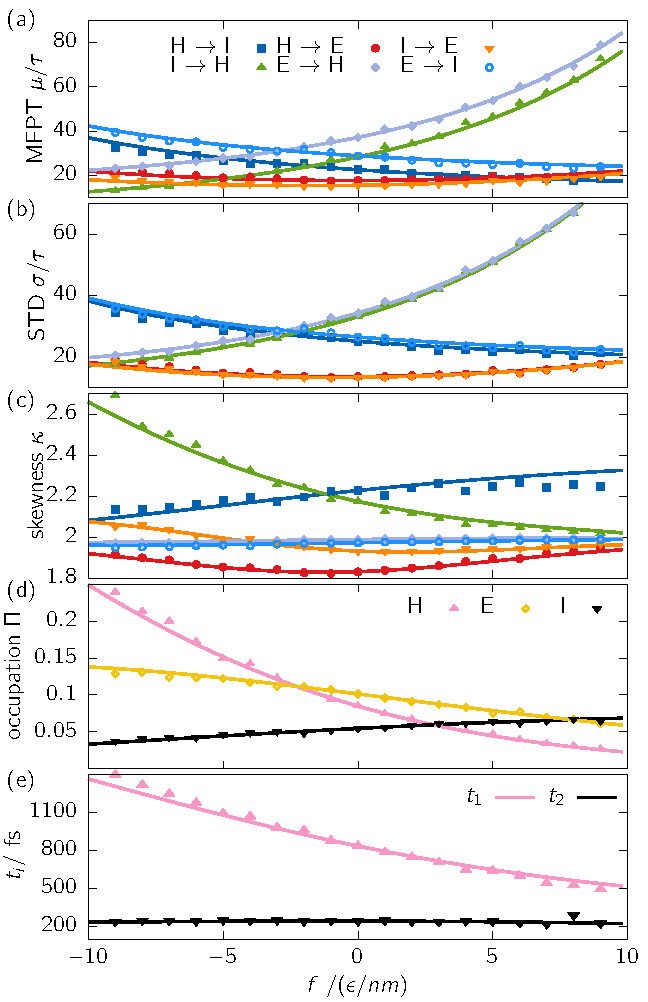
\includegraphics{../plots/Frew/mom_1001.pdf}
 \caption[The first three moments, the population of metastable states and the first two timescales for the tetraalanine peptide for varying driving along the end-to-end distance.]{(a-c) The first three moments of the FPTD for all six processes between metastable states defined in figure~\ref{fig:AlaLag} under varying external force $f$. (d) The occupation probability of each metastable state. (e) The timescale of the two slowest processes covered by the MSM. The dots represent the value measured from simulation. The line is the reference system continuously reweighted.   }
 \label{fig:momAlaR}
\end{figure}


 Figure~\ref{fig:momAlaR} shows the first three moments of the FPTD between the metastable states as defined in figure~\ref{fig:AlaLag}a. The metastable states as defined by PCCA+ do not coincide with the states highlighted for the eigenvectors. State H can be associated with  helical states, located to the right of the free-energy barrier at $\varphi \approx 0.15\,\pi$. State I is an intermediate state at $\varphi \approx 0.4\,\pi$. The global basin at extended state is not covered by the choice of PCCA+ because it is dynamically unstable. Nevertheless, we call the state identified below  extended state E. Transition from H or E to the intermediate state I slow down for attracting end-beads (negative forces) and speed up for repulsive end-beads (positive forces). The inverse happens for the processes from E or I to folded state H. Attractive end-beads increase the speed of these processes, driving to elongated states reduces it. H is the more stable configuration for negative driving because the end-beads can be close together. Transitions to extended state E are comparatively unaffected by the driving. Looking at figure~\ref{fig:momAlaR}d, the stationary distribution shows an increase in population of intermediates state I under repulsive end-beads. The extended state allows the end beads to be far apart and, therefore, it becomes more populated than state H or E.  The intermediate  state I and extended state E change linearly in probability with changing end-to-end attraction, the state H exponentially. The STD behaves proportional to the MFPT. The STD  shows minor changes under driving but does not show peculiar effects as seen for previous systems. The comparison is extended by the first two timescales of the system. The fast timescale depends strongly on the driving, the second timescale is unaffected as we have previously observed in the lagtime analysis. The systems analysed are in equilibrium and the dynamics are governed by accustomed detailed balance, so effects based on path-dependence are not expected. 
 
 The reweighting method works well for the tetraalanine system driven by a constant conservative force. Deviations are increasing for larger forces. This is based on high populations of regions with large and small end-to-end-distance, that are poorly sampled in the reference system. It is concluded that dynamics can be reweighted along the CV even if complex interactions of many bodies are involved.  This is based on the CVs chosen for the system give a reasonable representation for the dynamics of the system. The Maximum Caliber chooses the most uncertain system based on the information it gets. If the CVs chosen to describe the dynamics were insufficient, the Maximum Caliber would rely on insufficient data and produce wrong results. On the other hand, using information on the full conformational space would certainly include  irrelevant information for the chosen constraints. The Caliber would select highest uncertainty for these information. If the constraints were chosen correctly, this does not influence the result on the processes we are interested in. Well-chosen CVs delete information that the Caliber would ignore anyway, but we do not have to sample such information in the first place. In fact, the Maximum Caliber can be applied to choose CVs~\cite{smith2018multi,tiwary2016spectral}. The second input for the Caliber, the change in local entropy productions, can be estimate correctly because the driving is along a CV. Model-specific details on the trajectories --- like the density of trajectories or their local fluctuations --- are contained in the reference data. The new forces in CV space have to be applied to each of them irrespective of such details. 

\FloatBarrier
\subsection{Driving along Dihedral Angle}
\label{sec:DrivingDAla}
\begin{figure}[h]
 \centering
 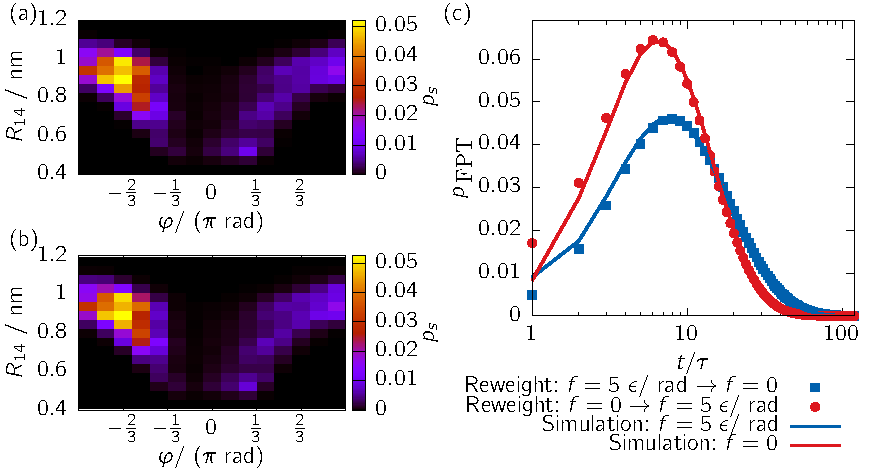
\includegraphics{../plots/Frew/single_2001.pdf}
 \caption[Stationary distribution and first-passage time distribution of a chosen process for tetraalanine peptide driven along the dihedral angle.]{(a) Simulated stationary distribution at $f = 0.8\,\frac{\epsilon}{\footnotesize{\text{rad}}}$. (b) Reweighted stationary distribution from reference to $f = 0.8\,\frac{\epsilon}{{\footnotesize \text{rad}}}$. (c) FPTD of driven and reference system for transition $H \rightarrow E$. The lines show data from simulation, the dots are from reweighting the systems into each other.}
 \label{fig:single2001}
\end{figure}



We will now turn to a driving along the dihedral angle. This is a circular motion with periodic boundary conditions giving rise to a NESS. While this force is artificial for the tetraalanine, such circular forces appear in molecular rotary motors. The rotation is driven by ATP-synthesis giving rise to a unidirectional motion of the molecule~\cite{fillingame1999molecular}.

The system is driven along the dihedral angle in both directions. Figure~\ref{fig:single2001} gives a detailed look at the system driven with $f =\,0.8 \frac{\epsilon}{{\footnotesize\text{rad}}}$. We note that the unfolded states are more populated than before and states to the right of the barrier are less populated. The FPTD distribution from helical states H to the extended state E is shown and captured by the reweighting procedure. Deviations can be seen for short processes of length  $1\tau$.  

\begin{figure}
\centering 
 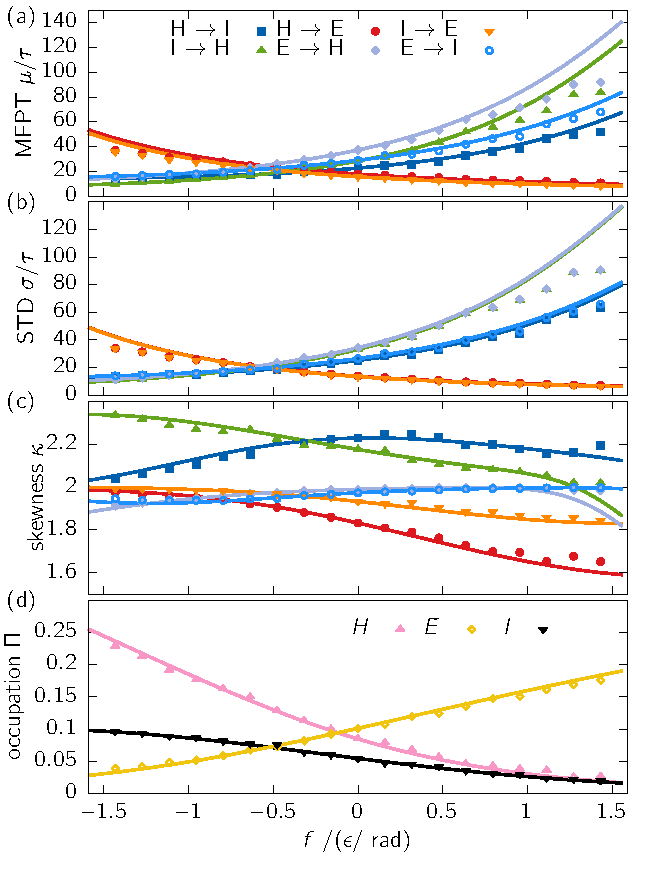
\includegraphics{../plots/Frew/mom_2001.pdf}
 \caption[The first three moments and the population of metastable states for the tetraalanine peptide for varying driving along the dihedral angle.]{(a-c) The first three moments of the FPTD for all six processes between metastable states in figure~\ref{fig:AlaLag} under varying external force $f$. (d) The occupation probability of each metastable state. The dots represent the value measured from simulation. The line is the reference system continuously reweighted.   }
 \label{fig:mom2001}
\end{figure}

Turning to figure~\ref{fig:mom2001} shows the driving along $\varphi$ in both directions. The dynamics of the system are largely dominated by its large centered free-energy barrier. Driving in positive direction, the processes H $\rightarrow$ E and I$\rightarrow$E become faster as they are connected along the periodic boundary.  The process I$\rightarrow$H slows down as it runs opposite to the force. On the other hand H $\rightarrow$I slows down, despite the fact that it runs along the external force. The trajectories bypass the state I under driving more frequently. The transitions I $\rightarrow$H and E $\rightarrow$H are not correctly recovered for larger driving by the reweighting. As expected, the dynamics slow down for simulation and reweighting for low forces. The simulation shows that the curve eventually reaches a maximum since the large barrier is crossed more frequently.  The reweighting procedure has problems capturing this effect correctly although it worked well for the single particle models. The STD follows the behaviour of the mean again and the skewness indicates that the reweighting works well for $|f|  <1\,\frac{\epsilon}{{\footnotesize\text{rad}}}$. Driving in negative direction the effect on dynamics is inverted. Processes aligned with the force speed up, whereas opposing processes are slowing down. The process H$\rightarrow$I does not follow this trend because it is accelerating too. The trajectories normally bypassing the state are now pushed into occupying the state. This is indicated by the increasing population of intermediate state I under negative driving  and depopulation under driving positive driving. The helical state population shows the same behaviour; the extended state shows inverse behaviour. The populations are recovered well by the reweighting, despite the deviations in the dynamics.  


\begin{figure}[t]
 \centering 
 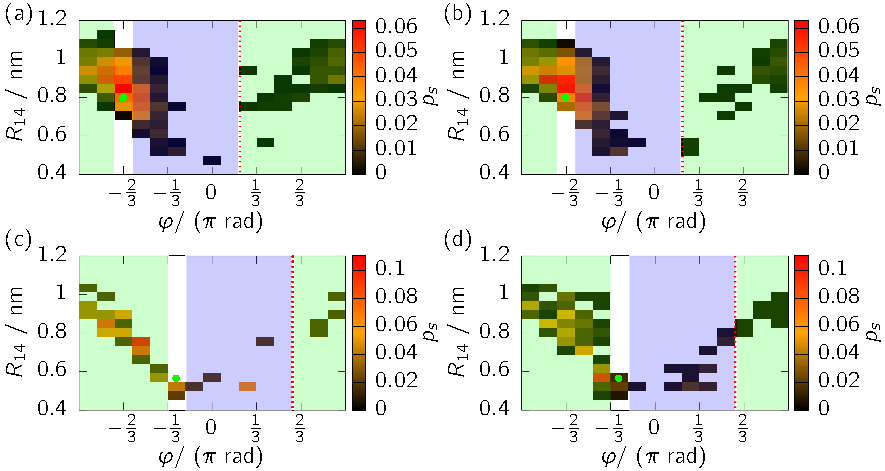
\includegraphics{../plots/Frew/Tv.pdf}
 \caption[Transition matrices of chosen initial point for the tetraalanine peptide reference model and a model driven along the dihedral angle. ]{Transition matrices, starting at the state marked by the green dot. The transition matrices left (a,c) show the reference systems, the right (b,d) show a system driven by $1.4\,\frac{\epsilon}{{\footnotesize\text{rad}}}$. The red line represents the discontinuity in local entropy productions, starting from the marked initial state. All states shaded green are connected to the starting state by trajectory going left, all states shaded blue are connected by a trajectory going right.  }
 \label{fig:dS}
\end{figure}
The reason for the described outlier lies in the local entropy productions. The correct choice is determined by the external force and the set of paths connecting every pair of microstates with each other. This connection of two microstates was straightforward to find for the previous system because they were separated by three or more barriers, as discussed in section \ref{sec:1Dmodel}. It was simple to determine if the collection of paths were directed with or against external forces. Such path dependence cannot occur for driving in $R_{14}$-direction in the previous section, because the origin of a path can be determined without periodic boundaries. This model on the other hand is driven to a NESS with periodic boundaries and shows only one major barrier along the dihedral angle. Choosing the correct local entropy production is more challenging here. For every jump in the Markov Model we have to decide if the underlying trajectory is aligned or directed against the external force. One approach to determine this is to analyse the trajectories as will be shown in section~\ref{sec:Trajectory}. Often one can deduce these information from the transition matrix as demonstrated in figure~\ref{fig:dS}a for the reference system. All states to the right (blue shaded) of the starting point are expected to emerge from trajectories in positive $\varphi$-direction, all states to the left (green shaded) in negative $\varphi$-direction,  taking periodic boundaries into account. In between these sets of trajectories is an area where no transition occurs. The lagtime of the MSM was chosen to be small such that these transitions do no take place, otherwise we were not able to tell whether the transitions occurred via a path going to the left or the right. This empty space acts as a dividing line between the two sets of trajectories, marked by the red dashed line. The connection between the states in the transition matrix indicate where to define the discontinuity in local entropy productions. Figure~\ref{fig:dS}b shows  the transition matrix with driving of $f = 1.4\,\frac{\epsilon}{{\footnotesize\text{rad}}}$ from the same  starting point as before. The transition probabilities change by the driving but the spatially long transition are still forbidden. We are able to tell if the transition took a path in negative or in positive $\phi$-direction. This is essential for the reweighting algorithm to work. For easier understanding it helps to have a look at the starting point of the transition matrix left to the large central barrier in $\varphi$-direction for the same systems in figure~\ref{fig:dS}c,d. The space can be separated in transition in positive and negative $\phi$-direction for the reference system, marked by the blue and green area. For the driven system however, we cannot decide if the Markovian jumps occur from hopping over the barrier or following a path around the periodic boundary. It might be that the microstates are connected by both sets of path. This makes it impossible to calculate the change in local entropy productions. Only if the set of paths are well-separated this is easily possible, as demonstrated for the first starting point. This is the source of the deviation seen in figure~\ref{fig:mom2001} for heavy driving.

We deduce that the reweighting along the dihedral angle will be limited for the present system. The set of paths connecting two microstates should consist of similar trajectories for reference and target systems.  The current system consisting of a single large barrier makes this difficult. Unfortunately, one cannot predict whether the aforementioned conditions are met. The small gaps between the groups of trajectories in Figure~\ref{fig:dS}a,b are a warning signal. Models with three or more barriers, as constructed as a toy model, are less susceptible for this problem. A particle crossing a barrier is expected to take the short path over one barrier and is unlikely to hop over two barrier within one lagtime. We may suspect that this problem occurs more frequently in small model systems with only few particles and less complex free energy surfaces. 

A possible way of solving this problem is by shortening the lagtime of the MSM. Shorter lagtimes result in shorter trajectories and shorter jumps. The reweighting procedure could be applied in a wider range. Unfortunately, figure~\ref{fig:AlaLag} shows that smaller lagtimes show non-Markovian dynamics. At the same time, increasing the number of microstates does not allow us to decrease the lagtime. Other choices made to construct the MSM are the CVs and the microstates. We may select a different second CV when reweighting along the first. Such choices have great impact on the system and solve the problem of missing free energy barriers.  The microstates in the present model are discretised in equal size along the CVs. Advanced clustering techniques like k-means~\cite{likas2003global} or k-medoids~\cite{park2009simple} help to define more complex sets of microstates that would allow to reduce the lagtime. Both, the selected CVs and the way of clustering the CV influence how dynamics are described by the MSM. We noted that the connection of two microstates should be described by a unique bundle of paths. This means that the CVs and its separation in microstates should be chosen to reflect underlying kinetic distances of the system. The same requirement for reweighting of dynamics in equilibrium was noted by Voelz et al.~\cite{wan2016maximum}.

We conclude that the reweighting procedure works for complex many-body-systems described by CVs. We show how the reweighting can be applied for conservative or non-conservative forces along the chosen CVs similarly. These forces might emerge from optical tweezers, molecular motors, mechanical dragging or any other type of disturbance. The reweighting is based on the combination of Maximum Caliber, information on reference data and local entropy productions on the target system. The CVs challenged the procedure by reducing the amount of information to a few variables. We have discussed for the driving along the end-to-end distance in section~\ref{sec:DrivingEAla} that the Maximum Caliber works irrespective of the coordinate system, provided the CVs contain the important information on the process of interest. In this section we have seen how the result is flawed based on inadequate constraints, whereas the underlying data is sufficient. Here, the physical choice of constraints is expected to be correct, but the constraints are flawed from a MSM construction point of view. 

% \FloatBarrier
% \bibliography{/home/marius/PhD/Thesis/references.bib}
% %\bibliography{../references}
% \bibliographystyle{plain} 
%  \end{document}    

% 
%% \documentclass[paper=a4,fontsize=12pt,open=right,noabbrev]{report}
% \documentclass[12pt]{report}
% \usepackage[utf8]{inputenc}
% \usepackage{amsmath}
% \usepackage{amssymb}
% \usepackage{graphicx}
% \usepackage{placeins}
% \usepackage{cite}
% \usepackage{physics} 
% \usepackage{mathrsfs} 
% \usepackage{geometry}  
% \usepackage{layouts} 
% \usepackage{newfloat}
% \usepackage{float}
% 
% \setlength{\parindent}{0em}
% \setlength{\parskip}{1em}
% 
% 
% % Technical point floatstyle
% \floatstyle{ruled}
% \newfloat{Technical Point}{htbp}{lop}[chapter]
% 
% 
% \begin{document}



\chapter{Complementary Aspects}
\label{ch:Complementary}
The described method was developed and constructed to reweight dynamical data in form of Markov State Models (MSM) between non-equilibrium steady states (NESS). The procedure in its current form is based on ideas from stochastic thermodynamics, coarse-graining of trajectories by MSMs and the Maximum Caliber. We want to discuss in this chapter how these ideas can be expanded in other applications than reweighting simulated data.

The defined ensembles and the parallels to equilibrium statistical mechanics raise the question if we can push this analogy further. In particular we will discuss if there is an invariant measure similar to the density of states (see section~\ref{sec:DoS}) that depends on the interaction of the system but not on thermodynamic variables. Other questions raised are the role of partition functions and the relation to thermodynamic variables based on derivatives. These relations in connection to the Maximum Caliber were discussed by Dill et al.~\cite{dixit2018perspective} for trajectory ensembles under global constraints.  Equilibrium statistical ensembles were also expanded to quantum mechanical systems. In combination with the discrete nature of MSMs, it can be beneficial to analyse such systems in the context of the presented ensembles. The laser system in section~\ref{sec:Lasersys} is such an example. It was approximated classically because simulation of quantum mechanical systems is beyond the scope of this thesis. 

The definition of the NESS ensembles is based on local entropy productions between discretised states. We will examine how this discretisation of dynamics is related to the underlying continuous trajectories. This will open up another way of estimating local entropy productions by trajectory averaging over an ensemble of single trajectories.

%At last we can discuss the construction of NESS-MSMs. Equilibrium MSMs can be constructed by inferring detailed balance on the data to converge MSM with less data available~\cite{bowman2009progress}. A similar approach can be applied here: Local entropy production and global balance were shown to be fundamental information on NESS ensembles. Enforcing them on a NESS would increase efficiency of MSM construction by inferring physical constraints.

\section{Invariant Quantity}
\label{sec:InvariantC}
An invariant has the property of not changing under a set of transformations. The density of states is one example under change of the Boltzmann measure (see section~\ref{sec:rewEqu}). It is defined by the number of microscopic states depending on chosen variables like energy and possibly other variables (see section~\ref{sec:DoS}). Once we have shown that systems are recovered under a certain transformation, we expect an underlying invariant measure. For the set of transformations used here, the \textit{dynamical invariant} was identified in section~\ref{sec:Invariant} by
\begin{equation}
    I_{ij}^2 = q_{ij} q_{ji} \exp \left ( \frac{c_i + c_j}{2}+ \zeta \right ) 
\end{equation}
and is presented for the minimal 1D system (see section~\ref{sec:1Dmodel}) in figure~\ref{fig:invariant}. Knowing the invariant of a system, one can construct any ensemble in NESS that we are interested in. The reweighting formula becomes
\begin{equation}
 p_{ij} = I_{ij} \exp \left ( \frac{1}{2} ( \tilde \zeta + \Delta S_{ij} )+ \frac{1}{4} (\tilde c_i + \tilde c_j)\right ),
\end{equation}
where $\mathbf{\tilde c}$ is determined by enforcing $\sum_k p_{ik}=1$ and applying the numerical solver used for the reweighting formula (see section~\ref{sec:numerics}). We want to understand the physical meaning of this quantity and show the technical use of it in enhanced sampling methods. 

\begin{figure}
 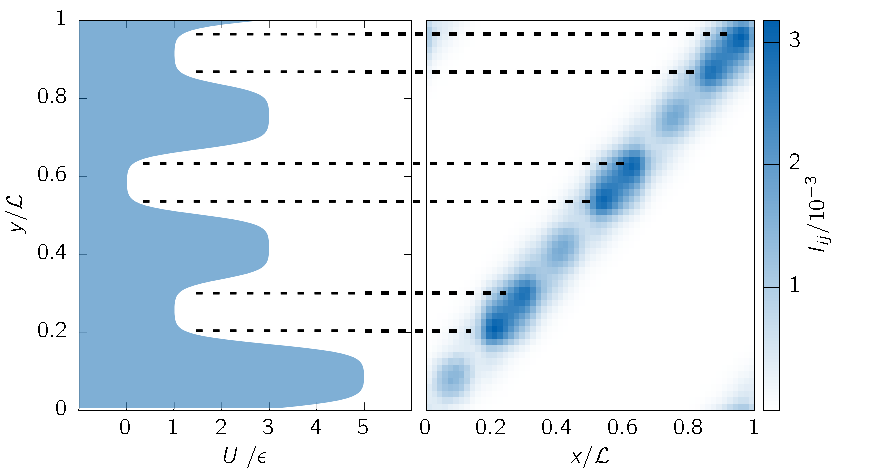
\includegraphics{../plots/Complementary/Invariant_2010.pdf}
 \caption[The dynamical invariant of the 1D driven system.]{The invariant of the 1D system. The potential surface is presented to indicate the positions of the maxima.}
 \label{fig:invariant}
\end{figure}

At first intuition the dynamical invariant is the density or number of trajectories connecting two microstates within lagtime $\tau$, equivalent to the density of states. However, this quantity is difficult to grasp because time and  length of trajectories have unknown relation without further information. We need thermodynamic properties like the diffusion coefficient $D = T\mu$, defined by the Einstein relation via temperature $T$ multiplied with the mobility $\mu$. For an ensemble of free diffusive single particles starting at position $X=0$ and time $t_0=0$ with diffusion coefficient $D$, the probability distribution at time $t$ is given by the solution to the Fokker-Planck equation~\cite{van1992stochastic}:
\begin{equation}
 P(X,t) = \frac{1}{\sqrt{4 \pi D t}} \exp \left (- \frac{X^2}{4Dt} \right ).
\end{equation}
The probability distribution is interpretable as the density of trajectories of length $t$ in free diffusion. The assumption  still holds for an invariant of NESS because a generalised diffusion coefficient was shown to depend on an effective temperature~\cite{lander2011mobility}. In any case, the invariant of the test 1D system in NESS in figure~\ref{fig:invariant} does not agree with the expected invariant. In fact it shows marks that originate from the potential and peak on top of the potential barrier and on the sides of the potential wells. The middle region of the potential wells show a lower invariant than its sides. This shows that the invariant depends on the temperature as expected but also on the potential surface. We believe that this dependence originates from the approximation used by the reweighting. A free diffusion invariant is expected for the full solution. An invariant for the full solution can be calculated if a numerical solution to the reweighting formula is found.


Nevertheless, the approximated invariant holds some information. We note from the definition that the matrix is symmetric. All information about dissipative effects are given by the local entropy productions.  The invariant on the other hand contains information about symmetric local fluctuations, or non-dissipative effect. These contributions were distinguished by Maes~\cite{maes2018non} showing that symmetric and asymmetric contributions to the dynamics are decoupled in equilibrium and coupled in off-equilibrium. The symmetric or \textit{frenetic} contribution can be defined by $A_{ij} = \sqrt{p_{ij}p_{ji}}$ such that $p_{ij}= A_{ij} \exp \left( \Delta S_{ij} /2 \right )$. The frenetic contribution changes with driving as predicted by Maes. The reweighting method uses information on dissipative dynamics but recovers these frenetic contributions correctly. We conclude that the invariant contains the necessary symmetric information. Accordingly we interpret the invariant as the non-dissipative local fluctuations of the system. 

This point of view explains why the reweighting scheme does not apply to temperature-reweighting. The chosen constraints infer information about  dissipative effects. The changes in the system under variation of temperature are in the non-dissipative part of the dynamics so it lies outside the scope of the presented method. It requires a different set of constraints that is unknown to us. 

The invariant is not completely understood, but it can be of computational purpose since it can be sampled from different simulations. This is the underlying idea of equilibrium enhanced sampling methods like multicanonical simulation \cite{janke1998multicanonical}, replica exchange \cite{sugita1999replica} or metadynamics\cite{laio2002escaping}. The general idea is to tweak the system such that regions of interest are sampled more frequently. This can be done by increasing the temperature to sample high-energy states more frequently or adding artificial potentials to push or attract the system in a certain direction. The changes do not have to be of physical nature and are removed from the system after taking advantage of better sampling conditions. All gathered information is collected in the invariant as long as the corresponding relations are known from a reweighting formula. These relations are for example based on the Boltzmann factor for the equilibrium ensembles or, here, the given reweighting relations for NESS.  The reweighting procedure can be combined with such sampling methods. This is a step to reach experimentally important timescales that are inaccessible by the limitation of computational power~\cite{perilla2015molecular}.

\section{Trajectory Analysis}
\label{sec:Trajectory}
MSMs are a coarse view on the dynamics of a system. The reweighting procedure acts on the MSM by enforcing the local entropy productions. We want to analyse how the single trajectories relate to the local entropy productions. The trajectory space allows us a detailed view on the system and one can judge if the microstate of the MSM and the assumptions for the analytic solution (see section~\ref{sec:Sprod}) are chosen correctly. The analytic solution ignores effects of fluctuations on the entropy production, the trajectory analysis takes them into account. Furthermore, the analytic solution for the entropy production only works when the new forces are applied along the collective variables (CV) chosen for the MSM. A trajectory analysis allows us to calculate entropy productions for forces depending on other system variables.
\begin{figure}
\centering
 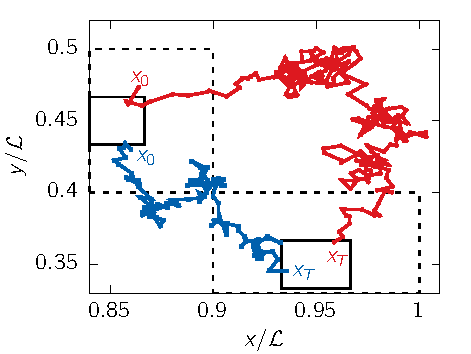
\includegraphics{../plots/Complementary/traj.pdf}
 \caption[Two example trajectories from simulation of the 2D system between two microstates.]{Two example trajectories from simulation of the 2D system between two microstates. The dashed boxes show the microstates, the solid boxes show the core of the microstates. A trajectory is counted when it starts and finishes in a core-state. }
 \label{fig:traj}
\end{figure}

MSMs are sampled by counting all trajectories that start in a given microstate $i$ and finish in another microstate $j$. The transition probabilities are defined by a trajectory ensemble average (see section~\ref{sec:StochTherm}) connecting two microstates
\begin{equation}
 \langle \chi_i (\mathbf{x}_0) \chi_j(\mathbf{x}_T) \rangle = \int \int \dd{\mathbf{x}_0} \dd{[\mathbf{x}(t)]} p [\mathbf{x}(t) | \mathbf{x}_0] p(\mathbf{x}_0) \chi_i(\mathbf{x}_0) \chi_j(\mathbf{x}_T) ,
\end{equation}
where $\chi_i(\mathbf{x})$ is $1$ if $\mathbf{x}$ is in state $i$ and $0$ else, $\mathbf{x}_0$ is the initial point of the trajectory~$\mathbf{x}(t)$ and $\mathbf{x}_T$ the final point. Similarly we  use this to calculate the local entropy production from trajectory space
\begin{equation}
\begin{aligned}
  \langle \Delta S \rangle_{ij} &=  \langle \chi_i (\mathbf{x}_0) \chi_j(\mathbf{x}_T) \rangle \\ &= \int \int \dd{\mathbf{x}_0} \dd{[\mathbf{x}(t)]} p [\mathbf{x}(t) | \mathbf{x}_0] p(\mathbf{x}_0) \chi_i(\mathbf{x}_0) \chi_j(\mathbf{x}_T) \Delta S[\mathbf{x}(t)] ,
\end{aligned}
\end{equation}
where $\Delta S[\mathbf{x}(t)]$ is the entropy production of a trajectory that is calculated by 
\begin{equation}
\begin{aligned}
  \Delta S [\mathbf{x}(t)] \approx \frac{1}{2T} \sum_d \sum_{t=1}^{t=T} \left ( x^{(d)}_t - x^{(d)}_{t-1} \right ) \left ( F^{(d)}({\mathbf{x}}_t) + F^{(d)}({\mathbf{x}}_{t-1}) \right )
\end{aligned}
\end{equation}
in discrete form, discussed in section~\ref{sec:Sprod}. The relevant trajectories are chosen  as illustrated in figure~\ref{fig:traj}. The dashed lines represent a microstate, the box in the middle is the core state. A trajectory starts in a core state and terminates when the final core state is reached. The center state ensures that fluctuations on the boundaries are not taken into account.  A maximum length of trajectory is set for computational efficiency.
\begin{figure}[t]
\centering
 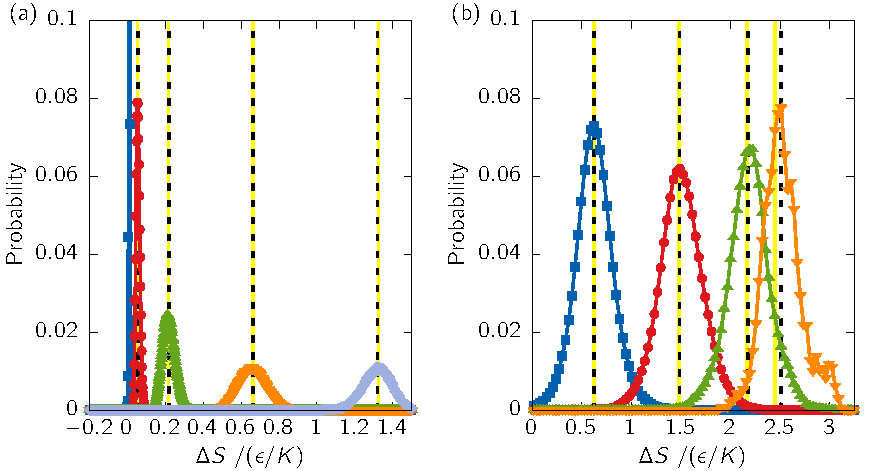
\includegraphics{../plots/Complementary/Shist.pdf}
 \caption[Distribution of entropy productions for the single particle in 1D potential and single particle in 2D potential for chosen transitions. ]{Distribution of entropy productions for (a) the single particle in 1D potential and (b) single particle in 2D potential for chosen transitions. The average of the distribution is shown by a black dashed line, the analytic solution is shown by a solid yellow line. }
 \label{fig:Shist}
\end{figure}
This does not influence the distributions of the entropy productions, shown for chosen transitions on the 1D and 2D model in figure~\ref{fig:Shist}.  The average of the distribution is shown by the dashed black line, the solid yellow line represents the average as calculated from the analytic model. The two values agree well, indicating that the analytic approximation works well on the coarse-grained level. Larger distances reduce the number of available trajectories and produce more noise. The full difference of analytic and measured value is shown in figure~\ref{fig:Sdiff} for the 1D system and locally for the 2D system.  We consider the trajectory analysis to be exact, because it takes all information into account and is sufficiently sampled for the given systems. The absolute deviations are small compared to the absolute entropy productions in the range $[-10\,\frac{\epsilon}{K},10\,\frac{\epsilon}{K}]$. Yet the 1D systems shows a pattern: When a trajectory start or ends in a state dominated by large local forces the deviation of the analytic solution is larger but still in an acceptable range. The deviation might originate from a non-symmetric distribution of entropy productions. This indicates that the fluctuations do not cancel each other out and the analytic assumption is flawed.  

A third way to estimate the entropy production is to use the transition probabilities of  the MSM by $ \ln \Delta S_{ij} = \frac{p_{ij}}{p_{ji}}$. This method agrees with the others but suffers from sampling issues for larger distances and needs longer simulation times to gather sufficient data, so it is not of further interest. The analytic method gives a good estimate and can thus be used for estimation of entropy productions without additional data used. The trajectory method can estimate the entropy production well but samples the whole distribution. It gathers more information than needed for the reweighting and requires simulation of the target system.  

The trajectory analysis is useful when one wants to reweight along forces not described by the CVs of the MSM.  The analytic method can only be used when the forces are defined on the same CV. Otherwise sampling the trajectories of the target system is the only way to estimate the target system for reweighting. One can sample the system at different thermodynamic states and gather the information at any of these states afterwards. Continuous reweighting is not possible in this case. The second use is testing for double peaks in the distribution of entropy productions. It indicates that two microstates are connected by more than one set of pathways. The MSM should be changed to resolve these pathways by a different choice of microstates. Otherwise the MSM is not able to distinguish all pathways and it would cause errors in the reweighting procedure. 
%The third use of the trajectory analysis is the efficient construction of MSM and is discussed in the next section

\begin{figure}[t]
\centering
 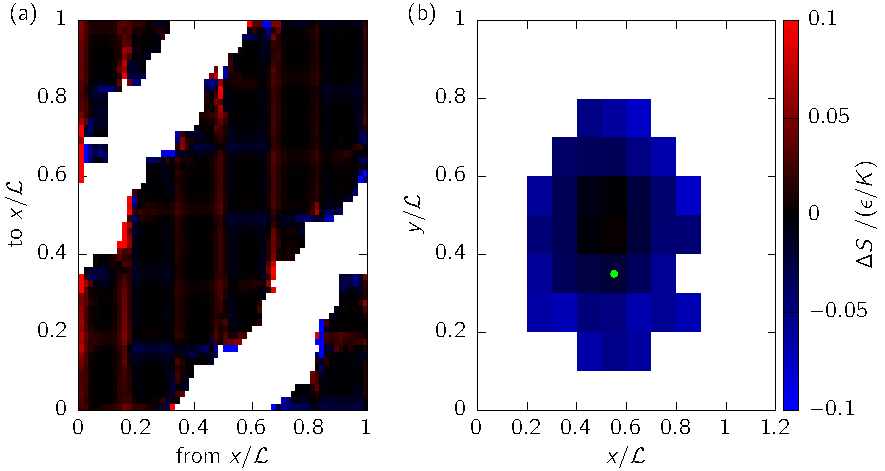
\includegraphics{../plots/Complementary/Sdiff.pdf}
 \caption[Deviation of local entropy production between analytic solution and averaging over simulated trajectories for (a) a single particle on a 1D potential surface and (b) a single particle on a 2D potential surface for a chosen starting point.]{Deviation of local entropy production between analytic solution and averaging over simulated trajectories for (a) a single particle on a 1D potential surface and (b) a single particle on a 2D potential surface for a starting point at (0.55,0.35), marked by the green dot.  }
 \label{fig:Sdiff}
\end{figure}


\section{Off-Equilibrium Reweighting in Literature}
Reweighting of dynamical data in and out of equilibrium has attracted some attention lately. Previous works were focused on reweighting dynamical ensembles of equilibrium systems, for instance using a Maximum Likelihood approach~\cite{chodera2011dynamical} or a Maximum Caliber approach~\cite{wan2016maximum}. It was shown how information can be drawn from non-equilibrium ensembles and combined at equilibrium~\cite{wu2016multiensemble}.  Here, we focus on the three works focussing on the problem for reweighting off-equilibrium dynamics. We want to discuss the assumptions of these methods and  compare them to our presented method. 

Two methods relying on the  Girsanov transformation~\cite{donati2017girsanov,warren2018trajectory} reweight each trajectory in conformational coordinates from the reference data individually. 
The first work by Warren and Allen relies on long trajectories and is tested successfully on a birth-death process in NESS. The authors point out two practical problems of the method: First they note that long trajectories are needed for unbiased reweighting and the length is set by the unknown target system. Second, the distribution of trajectory weights becomes broader with increasing trajectory length. These problems of long trajectories were avoided by Donati and Keller by employing short trajectories with Markov State Models. The method requires full data of the trajectories in conformational space and the random numbers generated during the simulation for the Langevin thermostat. Storing all this information would require large computational effort. In practice the lagtime of the MSM and the target state is defined before running the reference simulation and the trajectories are reweighted on runtime. It is  shown that the equilibrium MSM of a hexapeptide can be recovered. The method is combined with metadynamics~\cite{donati2018Girsanov} for efficient sampling of dynamics and construction of MSM. The reweighting method is in theory applicable for off-equilibrium MSMs, albeit it was not shown yet. In contrast, our method relying on the Maximum Caliber is applied a posteriori on an MSM. The target system can be chosen freely after the simulation data is gathered. The two methods mentioned above rely on reweighting every trajectory individually, forcing them to reweight during simulation runtime. Furthermore our method requires minimal computational effort by only solving a set of non-linear convex equations. The problem of long trajectories discussed by Warren and Allen was addressed by Markov State Modeling for both, the method of Donati and Keller and our method. 

Another new reweighting method applicable for NESS by Zuckermann et al.~\cite{russo2020iterative} was published by submission of this thesis. A number of short Markov-like trajectories are collected from a reference simulation. The target system for reweighting is defined by its stationary distribution. The weights of the reference trajectories are updated individually until they recover the target probability distribution and are stationary.  This algorithm can be extended to NESS by adding wells and sinks of probability at chosen positions. In this case the trajectories have to be arranged such that the probability is transported from well to sink while meeting the requirements on the stationary distribution. We refer to the paper for details of the algorithm. The method uses space discretisation like our method but does not require Markovianity unlike our method and the Girsanov reweighting. The trajectories are treated in their continuous form, similar to the Girsanov reweighting. This method was not yet tested on NESS systems.

The sparse number of works on reweighting dynamics off-equilibrium shows that it is a  new problem.  Most of the methods are only expected to work in off-equilibrium but are not tested yet. The presented methods rely on different theoretical bases and assumptions and operate on different spaces (long or short trajectories, MSM). We hope to see continuous work on this problem in the future.

%  to construct an MSM at equilibrium. It has been shown to be effiecient for a number of 


% \section{Markov State Model Construction}
% \label{sec:MSMCon}
% 
% 
% \bibliography{/home/marius/PhD/Thesis/references.bib}
% \bibliographystyle{plain}
% \end{document}

% \documentclass[12pt]{report}
% \usepackage[utf8]{inputenc}
% \usepackage{amsmath}
% \usepackage{amssymb}
% \usepackage{graphicx}
% \usepackage{placeins}
% \usepackage{cite}
% \usepackage{physics} 
% \usepackage{mathrsfs} 
% \usepackage{geometry}  
% \usepackage{layouts} 
% \usepackage{newfloat}
% \usepackage{float}
% 
% \setlength{\parindent}{0em}
% \setlength{\parskip}{1em}
% 
% 
% % Technical point floatstyle
% \floatstyle{ruled}
% \newfloat{Technical Point}{htbp}{lop}[chapter]
% 
% 
% \begin{document}
% 

\chapter{Summary}
The present thesis adds a new option for the sparse field of non-equilibrium steady states (NESS) reweighting of dynamics. It is built on the basis of Jaynes Maximum Caliber, an ensemble description of NESS by global balance an local entropy productions, dynamical information drawn from stochastic thermodynamics and coarse-grained dynamics by a Markovian assumption. The Maximum Caliber approach was chosen as it is a powerful tool for non-equilibrium processes. It was shown how reweighting relations between equilibrium ensembles emerge from the Caliber and we extended this idea to NESS. In fact the Caliber is under great discussion and its boundaries in the field of non-equilibrium physics are not yet determined~\cite{ghosh2020maximum}. 

We discussed how global or symmetric constraints describe the system inadequately. An equilibrium system can successfully be described by global constraints because its state is controlled globally, for instance by temperature or pressure. For a NESS on the other hand, the locality plays a major role: A system driven at its boundaries behaves differently from a system driven globally. The local entropy productions model these local effects and the amount of heat inserted to or withdrawn to or from the system. A global balance condition is added as a necessary condition for a NESS. It demands that the summed probability flows to a single state equals the probability of being in that state. This relates the dynamics to the statics of the system and ensures both to be time-independent, as required for a NESS. Furthermore, including  antisymmetric constraints are essential for the description of dissipative systems~\cite{agozzino2019minimal}.  We have shown that the combinations of these assumptions allow us to reweight between any NESS, including equilibrium systems.

This choice of constraints showed the existence of a symmetric invariant that contains information about the non-dissipative dynamics of the system. This quantity helps us to get a deeper understanding of NESS processes and the reweighting procedure itself. It contains the non-dissipative contribution to the dynamics that are drawn from the reference data.  We hope for deeper insight on the invariant and its relation to non-dissipative dynamics with an available full solution to the Maximum Caliber maximisation. From a technical point of view, sampling the invariant can be used to extend to an advanced sampling method for dynamics. Several systems can be computed at different thermodynamic states. For instance, artificial forces of varying strength can be added for improved sampling of a transition. All data can be combined in the invariant, possibly by weighting the data according to the local quality  of sampling, similar to weighted-histogram analysis method~\cite{kumar1995multidimensional}. 

The dynamics drawn form stochastic thermodynamics are described by Markov State Models (MSM) to control the enormous trajectory space of complex systems and perform the reweighting as efficiently as possible. A Maximum Caliber formulation on the trajectory space is possible but requires more sampled data and more computational resources due to the larger operating space. The Markovian assumption divides trajectories in small pieces and bundles them to a set of trajectories between two microstates. New trajectories are constructed from these pieces, possibly trajectories that are not existent in the reference simulation. In exchange for this reduction of space to sample, the MSM requires some knowledge of the system, for instance the collective variables (CV) have to be chosen appropriately to describe the dynamics of the slow processes. We recommend to discretise microstates fine enough to describe possible transitions between microstates by a spatially non-forking set of pathways. A trajectory analysis on the reference data reveals if the microstates are chosen sufficiently small by showing unimodal distributions. 

The Maximum Caliber approach was shown to apply to both, systems in full conformational space and systems described by CVs. The reweighting procedure works equally well because the maximisation only adjusts data that is significant for the chosen set of constraints. The entropy maximisation selects the distribution with the largest amount of uncertainty, so information that is not used in terms of constraints remain unchanged. Information significant to the constraints are adjusted, but the Calibers principle chooses the posterior to be as noncommittal as possible. Applying the Caliber to the full conformational space implies using data that is not needed to calculate local entropy productions. This data remains the same because no new information in form of constraints is provided and the Caliber maximisation produces the same answer. This property is used to find unknown collective variables for a system~\cite{smith2018multi, tiwary2016spectral}. 

The reweighting procedure in the presented form is designed to reweight with respect to forces along the CVs of the MSMs. Force-reweighting requires the underlying free energy barriers to be larger than the thermal fluctuations, i.e. $k_{\mathrm{B}} T < \Delta U$ and temperature reweighting is not possible.  Both types are  dominated by changing the non-dissipative dynamics, requiring a symmetric set of constraints. It would be of interest to identify these constraints and determine the relation to the anti-symmetric constraints used in this thesis. This would open up the reweighting procedure to temperature reweighting by symmetric constraints and to temperature gradients that should be described by a mix of symmetric and antisymmetric constraints or with no symmetry.  Reweighting methods in general are limited by the quality of the reference data since one does not know at what thermodynamic state the data are insufficient~\cite{warren2018trajectory}. Yet, we showed on several systems that reweighting works over a broad range of local and global forces. Our reweighting is applied to spatially short trajectories transitioning between microstates by use of the Markovian assumption. We benefit from short trajectories being easy to sample and more likely to be of importance in the target system, unlike long trajectories.

The small number of methods available as of now demonstrates the difficulties one is facing when dealing with off-equilibrium systems. Yet, the thesis showed that the Maximum Caliber is a powerful tool for understanding and analysing such systems. The presented models are small compared to complex systems exploiting the full range of computational resources available today. The thesis should be seen as a proof of concept for reweighting dynamics in NESS. Current MSMs are built for systems ranging from peptides to proteins, RNA and DNA~\cite{schutte2015critical} and the formulation in MSMs is expected to scale the reweighting method to such complex systems.
 
The method has a wide variety of possible application. We explained how it offers a way to perform enhanced sampling for dynamics of complex systems in NESS, e.g. molecular motors~\cite{schliwa2003molecular} or biological switches~\cite{goldbeter1997biochemical}. This allows to sample dynamics of more complex system without constraining the system to equilibrium. One might also use it to change details of an existing model: How does the dynamics change if an interaction is chosen differently? This provides information to improve coarse-grained models that do not show desired dynamic properties.  A comparable reweighting approach for coarse-graining systems was introduced by Shell et al., based on reference all-atomistic data~\cite{chaimovich2010relative}.  Furthermore, we discussed how the outcome of experiments like optical tweezers, mechanical dragging or activating a molecular rotary motor can be predicted. More applications on dynamical data from experiments are possible, the method only requires reference data on relevant CVs and a description of the forces or potentials applied. 
% 
%  
% \bibliography{/home/marius/PhD/Thesis/references.bib}
% \bibliographystyle{plain}
% \end{document}

  


% \documentclass[12pt]{report}
% \usepackage[utf8]{inputenc}
% \usepackage{amsmath}
% \usepackage{amssymb}
% \usepackage{graphicx}
% \usepackage{placeins}
% \usepackage{cite}
% \usepackage{physics} 
% \usepackage{mathrsfs} 
% \usepackage{geometry}  
% \usepackage{layouts} 
% \usepackage{newfloat}
% \usepackage{float}
% 
% \setlength{\parindent}{0em}
% \setlength{\parskip}{1em}
% 
% 
% %% Technical point floatstyle
% \floatstyle{ruled}
% \newfloat{Technical Point}{htbp}{lop}[chapter]
% 
% 
% \begin{document}
% 

\addchap{Samenvatting}
Dit proefschrift voegt een nieuwe element toe aan het bijzondere vakgebied van non-equilibrium steady states (NESS) reweighting van de dynamica. Het is gebaseerd op het principe van Jaynes' 'Maximum Caliber' (MC), een ensemble beschrijving van NESS door middel van globale balans en lokale entropie producties, dynamische informatie afkomstig van stochastische thermodynamica en grofkorrelige dynamica volgens een Markov aanname. De MC benadering is gekozen omdat het een krachtig instrument is voor niet-evenwichtsprocessen. Er werd aangetoond hoe herweging van relaties tussen evenwichtsensembles uit MC voortkomt en dit idee hebben we uitgebreid naar NESS. MC is een actueel onderwerp van discussie, en de grenzen van de zijn toepassingen op gebied van de niet-evenwichtsfysica zijn nog niet bepaald~\cite{ghosh2020maximum}.

We hebben beschreven hoe globale of symmetrische beperkingen het systeem onvoldoende karakteriseert. Een evenwichtssysteem kan met succes worden beschreven door globale beperkingen omdat de toestand ervan globaal wordt gecontroleerd, \mbox{bij}voorbeeld door temperatuur of druk. Voor een NESS daarentegen speelt de  locatie een grote rol: Een systeem dat aan zijn grenzen wordt gedreven, gedraagt zich anders dan een systeem dat globaal wordt aangedreven. De lokale entropieproducties modelleren deze lokale effecten en de hoeveelheid warmte die aan het systeem wordt toegevoegd of eraan wordt onttrokken. Een globale balansvoorwaarde wordt toegevoegd als noodzakelijke conditie voor een NESS. Het vereist dat de geaccumuleerde waarschijnlijkheid die naar een enkele toestand stroomt gelijk is aan de waarschijnlijkheid om in die toestand te zijn. Dit relateert de dynamica aan de statische eigenschappen van het systeem en zorgt ervoor dat beide tijdsonafhankelijk zijn, zoals vereist voor een NESS. Hiernaast is het betrekken van antisymmetrische beperkingen essentieel voor de beschrijving van dissipatieve systemen~\cite{agozzino2019minimal}. We hebben aangetoond dat de combinaties van deze aannames ons in staat stelt om te herwegen tussen alle NESS'en, inclusief evenwichtssystemen.

Deze keuze van beperkingen toonde het bestaan aan van een symmetrische invariant die informatie bevat over de niet-dissipatieve dynamica van het systeem. Dit helpt ons om betere inzichten te verkrijgen in de NESS-processen en de herwegingsprocedure zelf. Het bevat de niet-dissipatieve bijdrage aan de dynamica die wordt ontleend aan de referentiedata.  We hopen op een beter begrip van de invariant en zijn relatie tot de niet-dissipatieve dynamica met een beschikbare volledige oplossing voor de MC-maximalisatie. Vanuit een technisch oogpunt kan het bemonsteren van de invariant worden gebruikt om de aanpak uit te breiden naar een geavanceerde bemonsteringsmethode voor de dynamica. Verschillende systemen kunnen worden berekend bij verschillende thermodynamische toestanden. Zo kunnen bijvoorbeeld kunstmatige krachten van verschillende sterkte worden toegevoegd voor een betere bemonstering van een overgang. Alle data kan worden gecombineerd in de invariant, mogelijk door het wegen van de data volgens de lokale kwaliteit van de bemonstering, vergelijkbaar met de weighted histogram-analyse methode~\cite{kumar1995multidimensional}. 

De dynamica verkregen uit stochastische thermodynamica wordt beschreven door Markov State Models (MSM) om de enorme trajectruimte van complexe systemen te controleren en de herweging zo efficiënt mogelijk uit te voeren. Een MC formulering op de trajectruimte is mogelijk, maar vereist meer bemonsterde gegevens en meer rekenkracht door de grotere werkruimte. De Markov aanname verdeelt trajecten in kleine delen en bundelt ze tot een set van trajecten tussen twee microtoestanden. Uit deze delen worden nieuwe trajecten geconstrueerd, mogelijk trajecten die niet bestaan in de referentiesimulatie. In ruil voor deze verkleining van de te bemonsterde ruimte, vereist de MSM enige kennis van het systeem, bijvoorbeeld de collectieve variabelen (CV) die op de juiste manier gekozen moeten worden om de dynamica van de langzame processen te beschrijven. Wij raden aan om microtoestanden fijn genoeg te discretiseren om mogelijke overgangen tussen microstaten te beschrijven met een ruimtelijk niet-splitsende set van paden. Een trajectanalyse van de referentiegegevens laat zien of de microstaten voldoende klein gekozen zijn door unimodale verdelingen te tonen. 

De MC benadering bleek van toepassing te zijn zowel op systemen in de volledige conforme ruimte als op systemen die door CV's worden beschreven. De herwegingsprocedure werkt even goed omdat de maximalisatie alleen gegevens aanpast die significant zijn voor de gekozen set van beperkingen. De entropiemaximalisatie selecteert de verdeling met de grootste onzekerheid, zodat informatie die niet wordt gebruikt in termen van beperkingen ongewijzigd \mbox{blijft}. Informatie die significant is voor de beperkingen wordt aangepast, maar het MC principe kiest de posterior om zo \mbox{vrij}blijvend mogelijk te zijn. Het toepassen van MC op de volledige conformatieruimte impliceert het gebruik van gegevens die niet nodig zijn om lokale entropieproducties te berekenen. Deze gegevens blijven hetzelfde omdat er geen nieuwe informatie in de vorm van beperkingen wordt verstrekt en de MC-maximalisatie hetzelfde antwoord oplevert. Deze eigenschap wordt gebruikt om onbekende collectieve variabelen te vinden voor een systeem~\cite{smith2018multi, tiwary2016spectral}. 


De herwegingsprocedure die hier gepresenteerd wordt is bedoeld om de krachten langs de CV's van de MSM's te herwegen. Voor de herweging van de krachten is het nodig dat de onderliggende vrije energiebarrières groter zijn dan de thermische fluctuaties, d.w.z. $k_{\mathrm{B}} T < \Delta U$ en temperatuurherweging is niet mogelijk.  Beide types worden gedomineerd door het veranderen van de niet-dissipatieve dynamica, wat een symmetrische set van beperkingen vereist. Het zou interessant zijn om deze beperkingen te identificeren en de relatie te bepalen met de anti-symmetrische beperkingen die in dit proefschrift worden gebruikt. Dit zou de herwegingsprocedure openstellen voor temperatuurherweging door symmetrische beperkingen en voor temperatuurgradiënten die beschreven zouden moeten worden door een mix van symmetrische en antisymmetrische beperkingen of zonder symmetrie.  Herwegingsmethoden in het algemeen worden beperkt door de kwaliteit van de referentiedata omdat men niet weet in welke thermodynamische toestand de data onvoldoende zijn~\cite{warren2018trajectory}. Toch hebben we voor verschillende systemen laten zien dat herweging werkt op een breed scala aan lokale en globale krachten. Onze herweging wordt toegepast op ruimtelijk \mbox{korte} trajectovergangen tussen microtoestanden door gebruik te maken van de Markov aanname. We profiteren van het feit dat korte trajecten gemakkelijk te bemonsteren zijn en dat ze, in tegenstelling tot lange trajecten, eerder van belang zijn in het doelsysteem. 

Het kleine aantal methoden dat nu beschikbaar is, toont aan met welke problemen men te maken heeft bij niet-evenwichtssystemen. Toch toonde het proefschrift aan dat MC een krachtig instrument is om dergelijke systemen te begrijpen en te \mbox{ana}lyseren. De gebruikte modellen zijn klein in vergelijking met complexe systemen die gebruik maken van het volledige scala aan rekenfaciliteiten dat vandaag de dag beschikbaar is. Het proefschrift moet worden gezien als een proof of concept voor het herwegen van de dynamica in NESS. De huidige MSM's zijn gebouwd voor systemen variërend van peptiden tot eiwitten, RNA en DNA. De formulering in MSM's zal naar verwachting de herwegingsmethode opschalen naar dergelijke complexe systemen~\cite{schutte2015critical}.
 
De methode heeft een grote verscheidenheid aan mogelijke toepassingen. We hebben uitgelegd hoe het een manier biedt om verbeterde bemonstering uit te voeren voor de dynamica van complexe systemen in NESS, bijvoorbeeld moleculaire motoren~\cite{schliwa2003molecular} of biologische schakelaars~\cite{goldbeter1997biochemical}. Dit maakt het mogelijk om de dynamica van complexere systemen te bemonsteren zonder het systeem te beperken tot de evenwichtstoestand. Men kan het ook gebruiken om details van een bestaand model te veranderen: hoe verandert de dynamica als een interactie anders wordt gekozen? Dit levert informatie op om grofkorrelige modellen te verbeteren die niet de gewenste dynamische eigenschappen vertonen.  Een vergelijkbare herweging voor grofkorrelige systemen is geïntroduceerd door Shell et al., gebaseerd op referentie all-atomistische gegevens~\cite{chaimovich2010relative}. Verder hebben we besproken hoe de uitkomst van experimenten zoals optische pincetten, mechanisch slepen of het activeren van een moleculaire draaimotor kan worden voorspeld. Meer toepassingen met dynamische data uit experimenten zijn mogelijk, de methode vereist alleen referentiedata op relevante CV's en een beschrijving van de toegepaste krachten of potentialen.
  
% 
% \bibliography{/home/marius/PhD/Thesis/references.bib}
% \bibliographystyle{plain}
% \end{document}
  

  

\cleardoublepage 
\phantomsection
\addcontentsline{toc}{chapter}{List of Figures} 

\listoffigures 
\cleardoublepage 
%\setcounter{page}{113}
\phantomsection
\addcontentsline{toc}{chapter}{List of Technical Points}  
\listof{Technical Point}{List of Technical Points}
 

%\cleardoublepage 
%\begin{newenv}{Acknowledgements}
This dissertation marks the end of an exciting journey. I would like to express my deepest gratitude to a number of people that accompanied me during this time. 

My deepest appreciation goes to my supervisor Dr. Tristan Bereau, who supported me with his unlimited energy, his countless ideas and his ability to motivate and excite everyone around him. I enjoyed the freedom Tristan gave my in my research and his guidance whenever I needed it.   

I am deeply grateful to Prof. Dr. Kurt Kremer to accept me in his group at the Max Planck Institute for Polymer Research in Mainz. I appreciate his ability to give short lectures on any topic and always supporting me with his deep insight.

Special thanks to Prof. Dr. Evert Jan Meijer who became my second supervisor at the University of Amsterdam and supported me in the last chapter of my journey. I also thank the other members of my doctorate committee: Prof. Dr. Peter Bolhuis, Prof. Dr. Daniel Bonn, Prof. Dr.~ir. Marjolein Dijkstra, and Dr. Edan Lerner. 

I want to thank my colleagues for the countless discussion. A special thanks go to Prof. Dr. Burkhard D\"{u}nweg for sharing his knowledge with me and suggesting literature whenever I asked and to Dr. Joseph Rudzinski for all the discussion and his great support. I thank Kiran, Svenja, Bernadette, Christoph, Dominik, Bin, Marta, Martin, Roberto, Clemens, Anton, Claudio, Omar, Yasemin, Manjesh, Robin, Nezhat, Hannah, Debashish, Artreyee, Arghya, Marc, Alessia, Chan, and Timon for a great time at the Max Planck Institute for Polymer Research.

I would like to express my deepest gratitude to Prof. Dr. Wolfhard Janke, Dr. Thomas Neuhaus, Paul Spitzner and Dr. Johannes Zierenberg who taught me and discussed with me before and during my time in Mainz. 

Lastly I thank my brothers and my parents. Your unconditional support is the constant in my life and I am lucky to have such a great family. 


\end{newenv}


\cleardoublepage 
\phantomsection  
\addcontentsline{toc}{chapter}{Bibliography} 

\bibliographystyle{unsrt}
\bibliography{references}   

\todos 

\end{document}
\grid

